\documentclass[ % the name of the author
                    author={Elis Jones},
                % the name of the supervisor
                supervisor={Dr. Kirsten Cater},
                % the degree programme
                    degree={BSc},
                % the dissertation    title (which cannot be blank)
                     title={The Effect of Presentation Medium on Spatial Cognition},
                % the dissertation subtitle (which can    be blank)
                  subtitle={in the Virtual Environment},
                % the dissertation     type
                %  type={enterprise},
                % the year of submission
                      year={2018} ]{dissertation}
                
%% Language and font encodings
\usepackage[english]{babel}
\usepackage[utf8x]{inputenc}
\usepackage[T1]{fontenc}
\usepackage[margin=1cm]{caption}
\usepackage[table,xcdraw]{xcolor}
\usepackage{subfigure}
\usepackage[toc,page]{appendix}
\date{}

\usepackage{geometry}
\geometry{a4paper, portrait, margin=0.8in}

%% Useful packages
\usepackage{amsmath}
\usepackage{graphicx}
\usepackage[colorinlistoftodos]{todonotes}
% \usepackage{url}
\usepackage{caption}
\usepackage{multicol}
\usepackage{natbib}
\usepackage{listings}

\usepackage{color}

\definecolor{mygreen}{rgb}{0,0.6,0}
\definecolor{mygray}{rgb}{0.5,0.5,0.5}
\definecolor{mymauve}{rgb}{0.58,0,0.82}

\lstset{ 
  backgroundcolor=\color{white},   % choose the background color; you must add \usepackage{color} or \usepackage{xcolor}; should come as last argument
  basicstyle=\footnotesize\ttfamily,        % the size of the fonts that are used for the code
  breakatwhitespace=false,         % sets if automatic breaks should only happen at whitespace
  breaklines=true,                 % sets automatic line breaking
  captionpos=b,                    % sets the caption-position to bottom
  commentstyle=\color{mygreen},    % comment style
  deletekeywords={...},            % if you want to delete keywords from the given language
  escapeinside={\%*}{*)},          % if you want to add LaTeX within your code
  extendedchars=true,              % lets you use non-ASCII characters; for 8-bits encodings only, does not work with UTF-8
  frame=single,	                   % adds a frame around the code
  keepspaces=true,                 % keeps spaces in text, useful for keeping indentation of code (possibly needs columns=flexible)
  keywordstyle=\color{blue},       % keyword style
  language=Octave,                 % the language of the code
  morekeywords={*,...},            % if you want to add more keywords to the set
  numbers=left,                    % where to put the line-numbers; possible values are (none, left, right)
  numbersep=5pt,                   % how far the line-numbers are from the code
  numberstyle=\tiny\color{mygray}, % the style that is used for the line-numbers
  rulecolor=\color{black},         % if not set, the frame-color may be changed on line-breaks within not-black text (e.g. comments (green here))
  showspaces=false,                % show spaces everywhere adding particular underscores; it overrides 'showstringspaces'
  showstringspaces=false,          % underline spaces within strings only
  showtabs=false,                  % show tabs within strings adding particular underscores
  stepnumber=2,                    % the step between two line-numbers. If it's 1, each line will be numbered
  stringstyle=\color{mymauve},     % string literal style
  tabsize=2,	                   % sets default tabsize to 2 spaces
  title=\lstname                   % show the filename of files included with \lstinputlisting; also try caption instead of title
}
\bibliographystyle{agsm}

\parskip 4mm

\begin{document}

\iffalse
\section*{Prelude}
\thispagestyle{empty}
\fi
\maketitle
\frontmatter
\makedecl



\tableofcontents{}

\chapter*{Abstract}
The purpose of this study is to utilise the recent opportunities to construct more accessible virtual training environments, afforded by advances in hardware and software technologies; powerful game development platforms, 360-degree cameras, and VR headsets. These virtual environments have the potential to be utilised in multiple industries, this project focusses specifically on the charity lifesaving organisation for saving lives at sea, the RNLI. This plethora of new technologies lead to many different methods with which to construct a virtual training environment, this study aims to directly compare two methods; 360-image environment vs. computer modelled environment. These environments were constructed in Unity3D, the free game development platform. Users interacted with this environment using Google Daydream View. In order to conclude the most effective medium for training, this project focussed on training a user's landmark knowledge. A test was constructed where a user is required to memorise the location of 9 items within an environment. After completion, users complete a memory test, and again a week later. Results indicate that the computer-modelled environment was far more effective in training a user's landmark knowledge. It is theorised, although inconclusive, that this is caused by the difference of stereoscopic vision to monoscopic. Further studies are required to conclude the effect of context in which a user's required to recall their trained knowledge on a user's spatial memory, as well as the effect of stereoscopic vision.  

\mainmatter
\chapter{Introduction, and Background}\label{intro_chapter}
\section{Background}
\subsection{Royal National Lifeboat Institution}\label{rnli-money}
The Royal National Lifeboat Institution - RNLI - is a charity which save lives at sea. It is based in UK, Republic of Ireland, and the Channel Islands. In 2016, their crews and lifeguards saved 558 lives, with 8,851 emergency launches. Operating 238 lifeboat stations, and patrolling 240 beaches cost the institution £168.1M in 2015\footnote{RNLI: Where yours money goes \url{https://goo.gl/UjACQK}}. The cost of training a single lifeguard is £673, with the cost of a lifeboat crew member being considerably higher. \footnote{ RNLI Annual Reports and Accounts \url{https://goo.gl/XqhCZn}} 



\subsection{RNLI Training} \label{rnli_training}
The RNLI recruits and trains volunteers in order to save lives at sea. By the voluntary nature of recruits, it is not - and can not - be a requirement that a person has maritime experience prior to recruitment. Thus, the RNLI has a robust structure for crew development. Training consists of both theoretical training in a classroom, and sea-based, practical training.

The current format of training at the RNLI is that each crew member follows a structured training programme. This programme consists of multiple competence based training units, which cover an agreed range of skills required to complete a task. \footnote{RNLI: Lifeboat crew training \url{https://goo.gl/kuCafE}}. Each unit consists of a classroom theory element, and a practical element. For example, the first unit that a recently joined member of crew must complete is PPE, for which they are assessed on their knowledge of Personal Protective Equipment; this includes Helmet, Lifejacket, Flares, Personal Location Beacon, Harness, Dry Suit, Spray Hood, Whistle, and a Light. If a crew member is able to recall and describe each of these items and their function, they pass the unit and become eligible for assessment for the next unit - typically Boat Layout. 

Later units - such as Navigation - entail elements of both dry training (i.e. training on land) and wet training (i.e. training at sea). In order to pass the Navigation unit, a crew member must demonstrate their theoretical knowledge in a classroom test environment; for example, plotting co-ordinates on a map. The crew member will then be required to demonstrate their practical knowledge of the navigational equipment whilst aboard the vessel. 
For the previously described units, and for many similar units, the current training format is perfectly suitable for the training of inexperienced crew members; since there is no inherent hazard or significant cost to train a crew member to become competent at these tasks. This is not the case for all units. Units such as boat handling, sea survival, and capsize training - and many others - can become hazardous environments for inexperienced crew. This is due to the divide between theoretical training, and practical training. 

The current solution which the RNLI employs to bridge this divide between theory and practice is that all crew must attend a 1-week training course at the RNLI College in Poole. During this week, crew receive practical training in a specifically built facility; this training ranges through fire fighting, capsize drills, and sea survival. This process is expensive, but absolutely crucial to the safe functioning of Lifeboat stations. Due to the turnover of voluntary crew members, which increases the average costs of a fully trained crew member, It is not possible to frequently train crew in this manner. 

Scenario-based training is difficult to implement, because of the hazardous nature and potentially high cost of the scenarios for which a crew member must trained. Most notable of which is capsize training, an actual situation where a vessel capsizes will almost always be in terrible weather conditions, and sea state. But, unfortunately, the only way in which to replicate this in practice is by artificially capsizing a specifically designed vessel in a large pool or safe waters. This method is costly. Thus, an alternate method for which to replicate these situations would be invaluable not only the RNLI, but to all organisations which require training which is impractically hazardous or costly to conduct effectively.

The RNLI have already recognised this issue with current training techniques. At their headquarters in Poole, they have constructed an all-weather Lifeboat - ALB - simulator. This simulator consists of a large screen which is viewed from inside a model of the ALB wheelhouse. Using this simulator scenarios can be constructed such as fires, towing, poor weather conditions etc. Each of these scenarios would have been impossible to reconstruct without such an environment. This is a static simulator, with a cost far too high to allocate one for every station across the country; but this is certainly an insight into the necessity of such an environment.

\subsection{Technological Progress} \label{tech_progress}
The persistent march of technological innovation and progress present opportunities in every  industry, this is similarly true for practical training. Digitally simulated training environments are widely used, with the military and commercial aviation industries being the biggest investors. Training environments can be recreated in 3D as a simulator, allowing a user to be trained through a digital environment. 3D Simulators are not a new concept, but the creation of complex 3D applications has become considerably more accessible in recent years using free-to-use platforms such as Unity3D and Unreal Engine, and the ever increasing computational power of electrical devices. 

Of specific interest in this project is the more recent progress of Virtual Reality - VR - devices. This trend was reinvigorated by the development of the Oculus Rift - which was later purchased by Facebook \footnote{Facebook acquire Oculus \url{https://www.facebook.com/zuck/posts/10101319050523971}}. As with most innovations, the Oculus Rift is no longer the best selling headset, being replaced by the HTC Vive \footnote{HTC Vive Outselling Oculus Rift 2-to-1 \url{https://goo.gl/SfqrM2}} many other tech giants have released similar devices, such as the Samsung Gear VR, Google Cardboard, Playstation VR. With a fierce competition to capture a large share of a young market, pricing of high quality VR devices are falling year on year. Many VR devices - such as the Cardboard and Gear - take advantage of the power of modern high end smartphones. 

Creating 360-degree images and videos is now possible from most mobile devices, this can be done by stitching multiple images of a single scene together, in order to create a full image. Such methods construct a static 2D image, which can be interactively explored by a user. Dedicated cameras are becoming more widely available, utilising multiple omnidirectional cameras which capture video and automatically . The increased demand for 360-video lead to the largest video viewing platforms, YouTube and Facebook, both launching a feature in 2015 which allowed viewers to watch and interact with such videos \footnote{Facebook joins YouTube in showing 360-degree videos – including Star Wars \url{https://goo.gl/H9iE6f}}. 

In a similar manner to 360 photography, adoption of VR technologies has been rapidly increasing in recent years. With Facebook acquiring the VR company Oculus in 2014 \footnote{Facebook closes its \$2bn Oculus Rift acquisition. What next? \url{https://goo.gl/UQSTsP}}, and Google releasing its own VR interface for smartphones in the same year \footnote{Google Cardboard launches in UK for £15 \url{https://goo.gl/f9CS8f}}.  

With the time and cost requirement of both creating and interacting with 3D Virtual environments decreasing, there exists many opportunities for organisations such as the RNLI to utilise these technologies for training purposes. 

\subsection{Using Technology in Training }
The technological innovations mentioned in Section \ref{tech_progress} are offering new and fascinating ways to bridge the gap between theoretical and practical training.  These opportunities have not gone unnoticed by organisations such as the US Navy \citep{hussein}. Which conducted research in the 2009 into ways in which virtual environments could be implemented most effectively. The typical approach to a training system is to construct a 3D model of the vessel that the user can move through, and interact with, this is typically interacted with using a computer monitor, mouse, and keyboard. 

A computer generated - CG, virtual reality - VR, implementation of this seems like the natural progression of this, allowing a user to have a greater sense of presence. But, the recent development of 360 imaging presents a new opportunity to create a virtual training system, with far less software development expertise required. A simple application of 360 imaging for training could be that a trainee simply watched a 360 video through a VR headset, allowing the user to acquire a level of spatial awareness from a digital experience.

The two available approaches - VR and 360-imaging - offer clear benefits: VR allows a user to interact and manipulate a scene, and is dynamic; 360-video offers a photo-realistic representation of a scene. But, there are also economic factors which must be considered: VR requires software development expertise, therefore time and funding; 360-imagery can be created quickly, with relatively cheap equipment. Both require sufficient hardware, i.e. VR headsets, and computer systems or high-end mobile devices.  Hardware costs have been rapidly decreasing and can be expected to continue to do so. 

\subsection{Summary}\label{tech-summary}
In summary, modern technology offers opportunities to improve the way that the RNLI - and similar organisations - train their inexperienced recruits. But the broad list of available technologies to do this, reveal new opportunities to construct non-optimal solutions to these issues. By virtue of the broad scope of solutions, some effort must be made to research the most effective of them. This project will aim to clarify some elements of this. This leads in to the following questions:

\begin{itemize}
    \item \textit{Which technological approach, if any, is the most effective way in for the RNLI to train crew members?}
    \item \textit{What causes any disparity between these approaches?}
\end{itemize}

Thus, it is necessary to quantify the functional differences between these two approaches in the training of crew members. To do so, the current understanding of the field of psychology for practical training must be explored.

\section{Literature Review}\label{litreview}
First and foremost, it should be assessed whether it is appropriate to use virtual reality in order to train crew at the RNLI. \cite{Pantelidis2010} outlines the advantages and disadvantages of the use of virtual reality in training. In particular, the use of virtual reality is necessary when "training using the real thing is dangerous, impossible, inconvenient, or difficult"; many training units fit all but one of those criteria. Additionally, virtual reality training should be considered when "travel, cost, and/or logistics ... make an alternative attractive" and "teaching tasks involving dexterity or physical movement". In contrast, virtual reality should not be used when "interaction with real humans, either teachers or students, is necessary". Thus, the RNLI training programme is well suited to a virtual reality implementation of training, but careful consideration must be taken when deciding which units, and to what extent training will be completed in the virtual environment. 

These relevant units are reliant on a crew member's foundation of spatial awareness whilst aboard any vessel; a crew member must know the location of any equipment, the general geography of the local area - including hazardous areas above and below water. The acquisition of spatial awareness is referred to as spatial cognition, and is the foundation which allows a person to perceive, recall, alter, and communicate spatial information. It is therefore necessary to explore the current understanding of the function of spatial cognition in the virtual environment.

\subsection{Spatial Cognition}
According to \cite{stone}, the term spatial awareness can be applied to the immediate environment in which one exists or to a remote environment in which an extension of oneself has been deployed, such as a remotely operated vehicle or manipulator, or a virtual environment. Acquiring spatial awareness is a fundamental cognitive process which allows individuals to navigate any environment \citep{Michael2008}. Spatial cognition enables an individual to construct a cognitive map, from which they are able to determine the location of objects and themselves within an environment. \citep{downs}

 \cite{osberg} states that it is easy to assume that spatial cognition is a visual process, whereas it is in fact a multifaceted, multi-perceptual sequence of events.  The quality of distinctiveness or memorableness is not solely the result of the way the environment looks \citep{downs}. Although this is not a profound statement, it is important to consider, since the most intuitive view may be that the most accurate representation of an environment would be the most effective method for training. Given a scenario where only visual information is available, it would still not be necessarily true that the most accurate representation would be the most effective for training purposes. \cite{gleick} gives an interesting perspective, an artist's most powerful trait is realising that only a small amount of things are important, and they are able to see what they are. For direct sources of information, the visual, tactile, olfactory, and kinesthetic sense modalities combine to provide an integrated representation of the spatial environment \citep{downs}.

The widely accepted hierarchy for the development of spatial awareness is the landmark-route-survey hierarchy, first proposed by \cite{siegel}.  Landmark knowledge relates to the presence of dominant object, or groups of object. Route knowledge is the development of a familiarity of paths between landmarks. Survey knowledge is the integration of both landmark and route knowledge. Using these three sets of knowledge, an accurate representation of an environment can be compiled \citep{stone}.



\subsection{Training in the Virtual Environment}
The ultimate goal of training is to have an individual who is able to perform a desired task, and as said by \cite{hussein}, execute the necessary skills, quickly and without hesitation. This is absolutely crucial in the instance of the RNLI, since the trained tasks may be performed under high stress, in life-threatening scenarios. Training is most robust when it is habitual or automatic \citep{hussein}. This can be made possible by forcing trainees to over-learn a task, such that it requires minimal cognitive processing  \citep{kirlik}. Both environments that this study considers offer this feature, since they are both able to be used indefinitely by a user at no extra cost. 

\citet{osberg} identifies that a virtual environment - VE - offers a range of attributes which make it extremely well suited to training. Crucially, VEs offer an infinite amount of flexibility in the recreation of environments, This is trait which has been utilised since the original conception of VE-based training, and remains its most powerful. It is valuable to note, that although the 360-image environment is a virtual environment, it does support this flexibility; one of the most significant downsides to this method of training. 

Virtual environments allow a user to feel a sense of presence \citep{osberg}. Presence is the experience of a virtual environment, such that a user feels that they are "there" \citep{steuer}; presence is the sensation of being at a remote work-site rather than at the operator's control station \citep{Witmer1998}. In fact, the premise of virtual reality is to maximise the experience of presence to the point that a user is not aware that they are in a virtual environment. This accuracy relies on scale, position, and fidelity  of objects within that scene; secondly, it relies on the accurate and responsive display of the scene to the user; vividness and interactivity positively relate to the sense of presence \citep{steuer}. \cite{Gupta2008} agrees that "in order for these senses to be fully utilised and for knowledge to be transferred from the virtual environment to the real world, a high sense of presence must be experienced by the user". \cite{Witmer1998} found that there may be a weak but consistent relation between the sense of presence and task performance of users. \cite{Witmer1998} also states that immersion, selective attention, perceptual fidelity, and naturalness of interaction all affect a user's sense of presence. \cite{Romano2001} attempted to study these effects, but did not yield conclusive results; they do, however, posit that the type of interface is crucial to a user's training performance. Specifically, that head-mounted displays may offer a richer learning experience to users.

Interactivity is an attribute of virtual environments which may contribute to an improvement of a training system's success. Motor activity has a fundamental role in the acquisition of spatial awareness; interaction with an environment is absolutely necessary for the correct interpretation of that environment \citep{siegel}. \cite{osberg} stipulates that the ability to move freely is essential in order for an individual to form a spatial representation of an environment. Interactivity can be considered to be associated with the exploration mode of the user through the VE, either passive or active exploration. \cite{wallet} showed that active exploration may have a beneficial effect on spatial cognition. Although, according to \cite{wallet} studies of these two strategies of exploration offer inconclusive results, and may be a result of varying complexity of tasks. This may be contradictory to training theory according to \cite{goldstein}, who states that any complex task must be broken into smaller tasks which can be individually trained to proficiency before integrating these learnt skills to the entire complex task. Which leads to a dilemma: active exploration may be more effective for complex tasks, but training is generally more effective when complex tasks are divided and conquered as simpler tasks. For further complexity, \cite{waller} found that VEs are more effective than real world training only after extensive exposure to the training environment. As such, the complexity and length of the training exercise will be a crucial factor to be considered when constructing an application and during the study. 

\subsection{The Effectiveness of Training in Virtual Environments}
"It is important that the environment in which a child is expected to learn be conducive and supportive of the learner" \citep{osberg}. A virtual environment enables this support, since the environment can be manipulated to any extent necessary to achieve this. \cite{Rose2000} studied the true potential for training that virtual environments had. They concluded that virtual environments were in fact an effective way to train individuals, with there being no discernible difference in  the performance of individuals trained in the real world and in a virtual environment. More interestingly, participants trained in virtual environments coped better with interference when performing the task. \cite{Rose2000} hypothesise that this may be due to the nature of real world tasks being more mentally taxing, requiring more mental capacity, any added interference becomes difficult to handle; whereas, virtually trained participants have spare cognitive capacity. Other studies such as \cite{Hamblin2006} only concluded that training in the virtual environment was effective, but not as effective as training in the real world. \cite{Gupta2008} summarises that virtual environments are most useful for training in dangerous or costly tasks, but that virtual environments would never replace training in the real world for tasks which do not have these limiting factors. 

\subsection{Summary}\label{intro-summary}
It is clear that there is a multitude of factors that have an effect on spatial awareness which is developed in a virtual environment. With respect to human senses, almost every sensory modality plays a part in a user's ability to acquire spatial awareness. Utilised senses are reduced to only visual and motor activity when a user is within a virtual environment. The key factors which may enable effective acquisition of spatial awareness are presence, and interactivity. 

The elements of spatial cognition and the construction of cognitive maps discussed above are perfectly suited for modern virtual reality environments. Most notably, the ability for natural movement within a scene has progressed in leaps and bounds in recent years. Modern devices offer head-tracking on motion-tracked controllers, allowing users to interact with an environment in far more complex ways than previously possible.

Presence is a factor which has proven difficult to quantify, or study. But, modern devices offer many of the features which have been discussed to be necessary in order to yield a satisfactory sensation of presence within a virtual environment. Powerful computers enable the construction of more accurate 3D models than ever before, which is a feature deemed invaluable by previous studies \citep{steuer}. 

Further, the elements of virtual training environments which make them potentially more powerful than real world training environments are infinite flexibility, and the ability to repeat scenarios indefinitely at no - or minimal - added cost, and completely without danger. Reinforcing the idea that virtual environments are the perfect addition to many training programmes that exist within organisations such as the RNLI.


% Discuss Context!!!
\chapter{Approaches, and Requirement Analysis}

\section{Requirements} \label{requirements}
\subsection{User Study}
In order to reach a robust result it is important to detail the requirements of the user study. Crucially, the environment should be as consistent as possible between the two groups. The requirements follow:

\begin{itemize}
    \item Identical hardware
    \item Similar environment for all but presentation medium
\end{itemize}

\subsection{Application}
As discussed in Section \ref{litreview}, virtual environments offer effective ways to train users. In particular, environments which are associated with excessive costs, and hazardous scenarios benefit most from such environments. The RNLI is an ideal candidate for such a training environment to be implemented. With this in mind, the requirements - as detailed by Section \ref{litreview} - of such an application are as follows:

\begin{itemize}
    \item Affordable
    \item Accessible
    \item Effective
\end{itemize}

Affordability is an inherently relative requirement. In this instance, an opportunity to improve the performance of every crew member at a lifeboat station would be extremely valuable to any lifesaving organisation. But, the RNLI already spends large amounts of resources on training as discussed in Section \ref{rnli-money}. Regardless, it is an important consideration to be aware of throughout this project. An accessible solution ensures that it could be rolled out to all stations without the need to invest resources and time to train each station how to set the virtual environment up. The requirement of an effective solution means that it should be able to effectively train crew, and improve their performance in the assessment of competency based units. In order for a virtual environment to effectively train individuals the following requirements must be considered:

\begin{itemize}
    \item Users must feel present within the environment.
    \item Users must be able to interact naturally with the environment.
    \item The environment must accurately represent the scale and position of objects within it.
\end{itemize}

\section{Approaches}
\subsection{Technology}
In consideration of the aforementioned requirements, modern technology offers two methods to place trainees in interactive virtual environments, 360-degree imaging, and computer-generated virtual reality; although 360-degree imagery is often disputed to be a form of VR \footnote{STOP CALLING GOOGLE CARDBOARD'S 360-DEGREE VIDEOS VR \url{https://goo.gl/UGthLf}}, the two technologies will be referred to as 360 and CG for simplicity. 

\subsubsection{360 Imaging}
The RNLI has experimented with 360-imaging in the past, creating a tour of their new Shannon-class All-weather Lifeboat \footnote{RNLI VR Tour, for Cardboard \url{https://goo.gl/1Ha6vs}}. This application allows a user to explore a series of 360 images from within the vessel. This application also offers some level of interactivity, which may be moderately effective in the training of crew members. Although, according to previous studies interactivity, and active exploration may be essential to effective training. This application uses static images which can be collected with the use of an omnidirectional, monoscopic camera; monoscopic means that the image produced is a single image not two images taken at slightly different locations. Since this is monoscopic, it is not possible to make a 3D scene, and only a 2D environment. At the very cutting edge of 360-imagery, stereoscopic cameras are available, although the current cost is considerably higher than the simpler monoscopic cameras; this cost - as with any modern technology is rapidly declining \footnote{Forbes: China's Kandao \url{https://www.forbes.com/sites/bensin/2018/05/02/chinas-kandao-says-its-triple-lens-360-cam-can-shoot-3d-vr-footage/#1b64d8524fd2}}. Furthermore, the added complexity for manipulating stereoscopic imagery is beyond most free software, although there are many applications which do offer this functionality \footnote{Nvidia: 3D PC Editing Software\url{http://www.nvidia.co.uk/object/3d-pc-editing-software-uk.html}}. 

In light of this, in order to fulfil the two previously discussed requirements, accessibility and affordability, a monoscopic 360 camera is the only option within the scope of this study. Although, this has a potential to reduce the overall effectiveness of the application, since a user will have a reduced sense of depth. This difference is discussed in Section \ref{stereo}.

\subsubsection{Computer Generated Virtual Reality}
There is an expansive list of potential applications which could be used to develop immersive, interactive, 3D environments. Many of these platforms are free for use, or follow a freemium business model. The most popular of which are Unity and Unreal Engine \footnote{Instabug: Game Engines \url{https://blog.instabug.com/2017/12/game-engines/}}; there are also open-source solutions such as Godot. Each of these engines fit the aforementioned requirements, and are fully capable of constructing and effective VR application. 

Similarly, there is an abundance of applications available for the construction of 3D models. Most notable of which are Blender, and Maya. Blender is an open-source 3D modelling suite, whereas Maya is a professional 3D modelling suite. Both are fully capable of constructing the necessary models. Maya offers a free student license, and thus will be used for the creation of 3D models throughout this project.

\subsubsection{Viewing Hardware}
In conjunction with the requirement of consistency between environments, it is necessary that both applications should be experienced using identical hardware. Viewing virtual reality environments is done using a head-mounted display - HMD - as shown in Figure \ref{headmounted}.

\begin{minipage}{\textwidth}
\centering
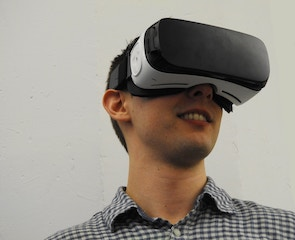
\includegraphics[width=0.6\textwidth]{images/headmounted.jpg}
\captionof{figure} {Head-mounted display. Device shown is the Samsung Gear VR.}
\label{headmounted}
\hfill \break
\end{minipage}

Due to the thriving nature of the virtual reality market, there exists many options when it comes to selecting a device. In order to experience a simple scenario based training environment, it would be unnecessary to select high-end HMDs to do this. The cost of high-end HMDs do not truly demonstrate the cost associated with owning one. High-end HMDs require the use of similarly high-end computers, making the devices less affordable, and less accessible. The total cost of a HMD and VR-capable PC sitting at a minimum of £750 \footnote{VRHeads: What is the total cost of an HTC Vive \url{https://www.vrheads.com/what-total-cost-htc-vive}}. A final drawback to such devices is that they are tethered - i.e. they must be wired to a VR-capable PC. This means that crew would be unable to utilise these training devices outside of a designated training space, leading to much less flexiblity for training. 

The alternative to such tethered, high-end HMDs are Mobile VR HMDs. Typically mobile HMDs utilise smartphone devices to display a virtual environment; although more recently, the Oculus Go was announced which does not follow this trend \footnote{Oculus Go \url{https://www.oculus.com/go/}}. These devices offer a perfect combination of accessibility, flexibility, and affordability. The only prerequisite for using the device is a modern smartphone, making the device accessible. The total cost of a dedicated VR experience would typically be £450, including a dedicated smartphone device \footnote{Amazon: Samsung S8 \url{https://www.amazon.co.uk/Samsung-SM-G950F-64GB-SIM-Free-Smartphone-Midnight-Black/dp/B06XYMCMHD/ref=sr_1_1?s=telephone&ie=UTF8&qid=1525428029&sr=1-1&keywords=samsung+s8}}\footnote{Google Store: Daydream View \url{https://store.google.com/gb/config/google_daydream_view}}. Following from this, a Mobile VR HMD will be the hardware used in this project.

\section{Application Design}
This project aims to construct a proof-of-concept application which allows a user to reach a level of competence to pass a unit which they are assessed for. In addition to this, the application should enable a quantitative comparison to be made between the two methods of presentation; 360-imagery vs. computer-generated. To do this compromises must be taken which make the two applications more directly comparable. 

\subsection{Assessment Units}
As discussed in Section \ref{rnli_training} the training programme of crew members at a RNLI Lifeboat station is composed of a series of competency based units, which they are assessed for. This training programme will take a new recruit from an inexperienced crew member to a fully capable coxswain - the most senior role of crew, who is responsible for managing crew on an ALB. 

The first stage of a new recruits training programme involves training to a level where they are capable to go to sea without endangering themselves or other members of crew. This stage consists of only dry training - on land. The following units must be completed to reach this point:

\begin{itemize}
    \item Personal Protection Equipment
    \item Roles and Responsibilities
    \item Boat Layout
    \item Medical Assessment
\end{itemize}

\subsection{Boat Layout}
Boat layout is the assessment of a crew member's knowledge of the location, and function of every piece of equipment aboard the vessel which they will be a crew member for. This knowledge is crucial to the safety of any person aboard the vessel, and it is essential to the safe operation of the vessel. This project will focus on the most common vessel in the RNLI fleet, the D-Class IB1 type, with 135 vessels in service across the country \footnote{RNLI: D-Class \url{https://rnli.org/what-we-do/lifeboats-and-stations/our-lifeboat-fleet/d-class-lifeboat}}. The equipment on the D-Class consists of over 20 different objects. 

\subsection{Application}\label{application-approach}
Boat layout is an appropriate unit to implement for training, as it allows for both a realistic approach to how the application could train a crew member. In addition, the effectiveness of this training would be  quantifiable, and thus a robust user study could be conducted with it. This application must enable a user to explore the D-Class, and inspect the equipment which is on board.

Now that the unit for assessment has been chosen, it is necessary to decide the way in which user's will be assessed for their performance, so that an appropriate application can be constructed. In brief, the user study will require users to recall the location of the items aboard the vessel - the design of the user study is discussed in detail in Chapter \ref{user-study-chapter}. In order to enable a fair user study to be conducted some compromises must be taken from the realism of the layout of the vessel. The number of items of equipment must be reduced, and in accordance to Miller's Law the most appropriate number of objects would be nine in this case \citep{Miller1956}. 

\chapter{Development}

\section{Application Overview}
The requirements for this application were to construct two environments within which users are able to explore. Crucially, these applications should be interacted with in the same way and use the same hardware, in order to not introduce uncontrolled variables to the study. Additionally, in order to avoid motion sickness in users both environments will not allow for continuous adjustment of location in the environment. Thus, users will only be able to move discretely throughout the scene by selecting locations they wish to move to. 

Broadly, the intention of this project is to construct a virtual training environment in order to train crew members on RNLI Lifeboats. As discussed in Section \ref{tech_progress} there has been significant progress in the field of immersive virtual reality environments. Specifically, this application will teach users the layout of the equipment aboard the vessel. As detailed in Section \ref{application-approach} the number of items the user will need to recall the location of will be nine. These nine items are as follows:

\begin{itemize}
    \item Anchor
    \item Compass
    \item First Aid Kit
    \item Gloves
    \item Handheld Radio
    \item Light
    \item Propeller
    \item Tow Rope
    \item VHF Radio
\end{itemize}

\section{Technical Overview}
As indicated in Section \ref{requirements} a crucial aspect of each of the environments, is that they can be constructed using modern, affordable, and easily accessible tools. As such, it is an easy decision to utilise the Unity3D game development platform. In conjunction with the use of Unity3D, Google offers a fantastic library for development on their Google Cardboard and Daydream platforms. In order to construct the 3D Model of the D-Class, the 3D modelling and animation software Maya is used. 

In order to collect memory test results remotely for users, Github Pages was also utilised, which is a free platform on which to host static websites. Data storage, and user information was handled by the Google APIs Firebase, and OAuth2.

\section{Computer-Generated Environment}
\subsection{Modelling}
This project required the construction of two applications. First of which, the CG environment utilised 3D models constructed in the professional 3D computer graphics application Autodesk Maya. These models are then imported into the free-to-use cross-platform game-engine, Unity. Utilising the Google VR SDK, a VR application is constructed. Unity is able to build to the Android platform. Using an android device and a Google Daydream View Headset, users are able to interact with the constructed environment.

\subsubsection{Boat}
A crucial factor of any virtual environment is scale. In this case, it was important that the 3D-model of the vessel was true to life. Maya offers fantastic tools to enable this, namely tracing over image planes. Imported images of the object being reconstructed are overlaid onto the workspace and set to be partially transparent. Using the orthographic view, the image can be perfectly traced to match the object. This is demonstrated in Figure \ref{image-plane}. 

The vast majority of elements in the D-Class model can be constructed using the polygonal primitives. These primitives are enough to construct highly complex models, if used in conjunction with soft selection, and smoothing.

\begin{minipage}{\textwidth}
\hfill \break
\centering
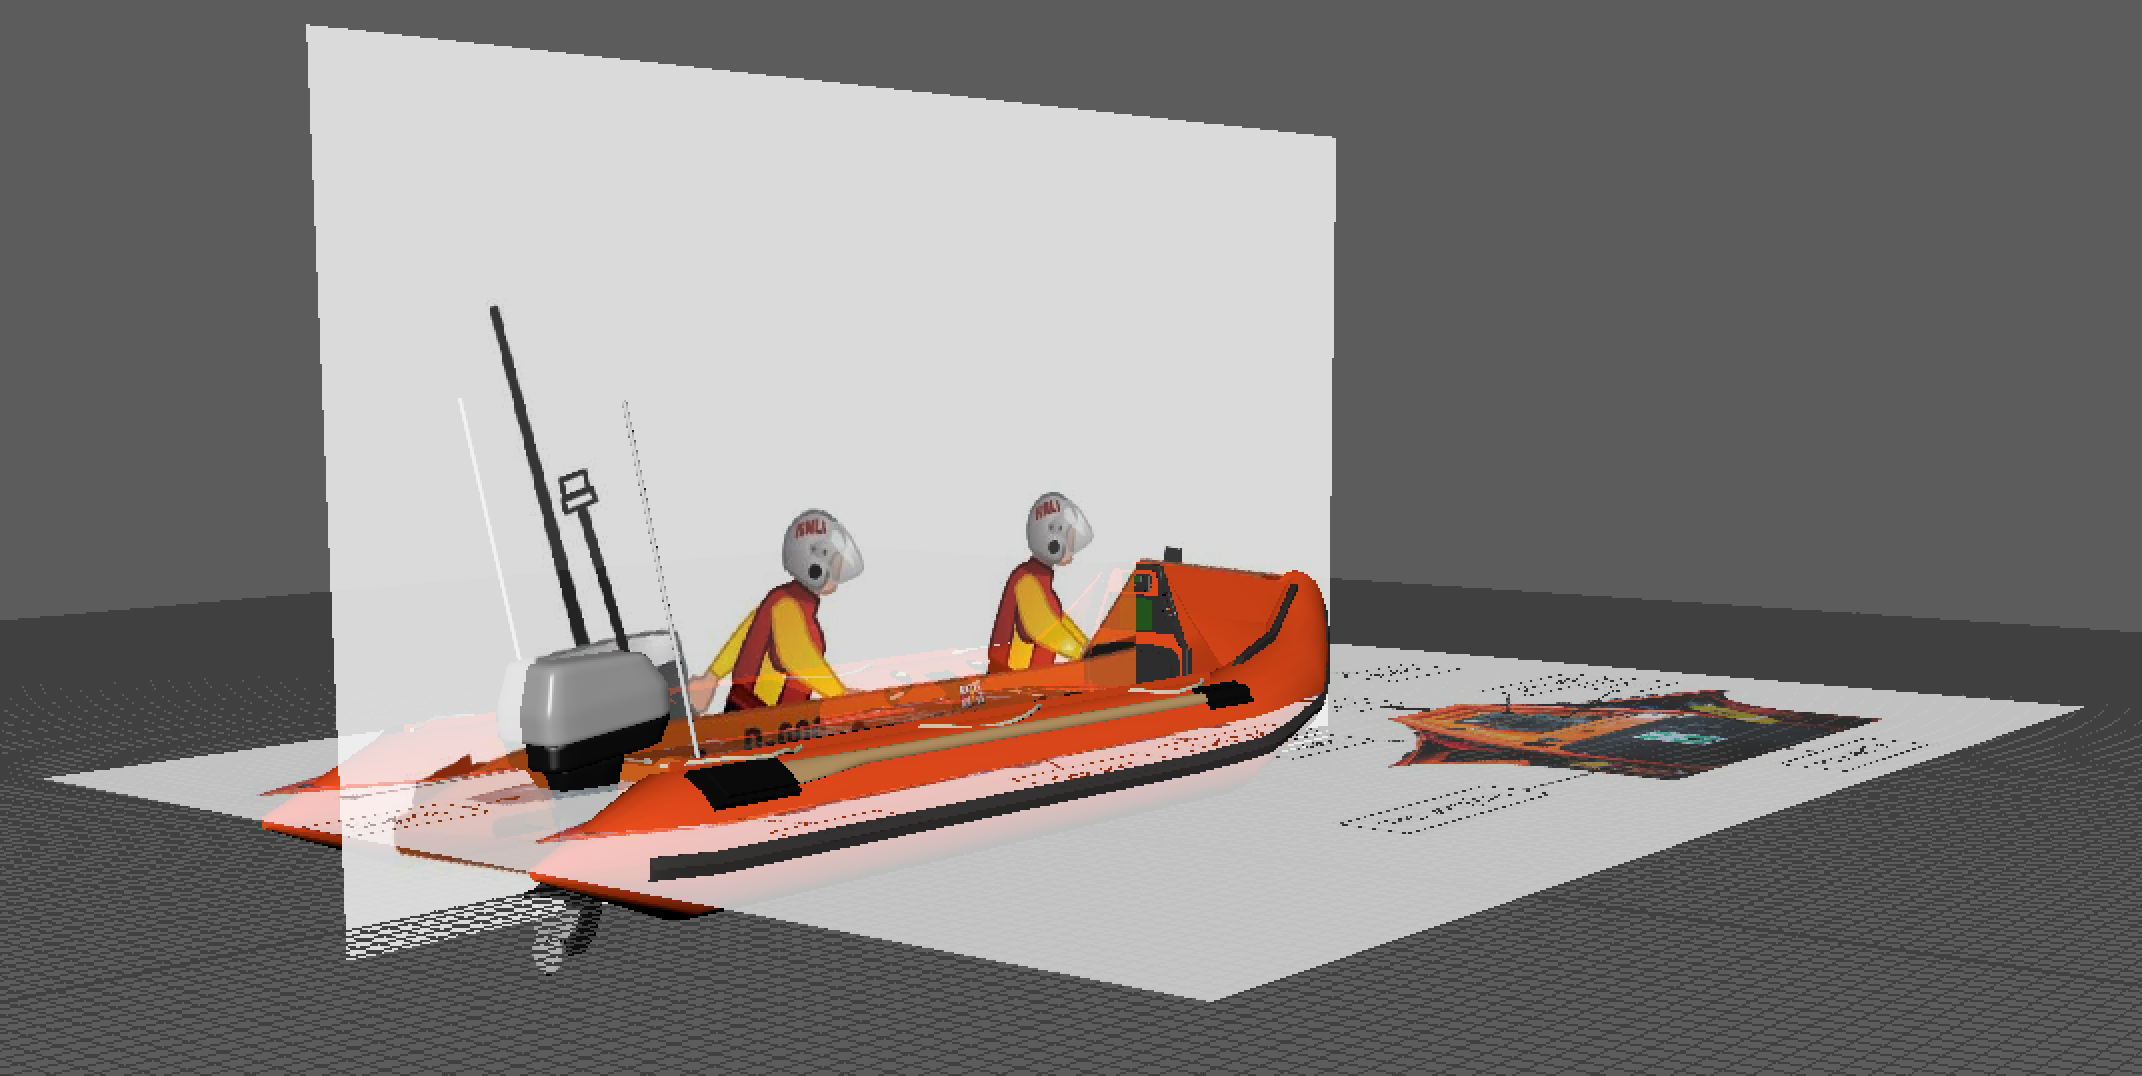
\includegraphics[width=0.6\textwidth]{images/image_planes}
\captionof{figure}{Screenshot of image planes overlaid onto the 3D model, shown in perspective view}
\label{image-plane}
\hfill \break
\end{minipage}

\begin{minipage}{\textwidth}
\hfill \break
\centering
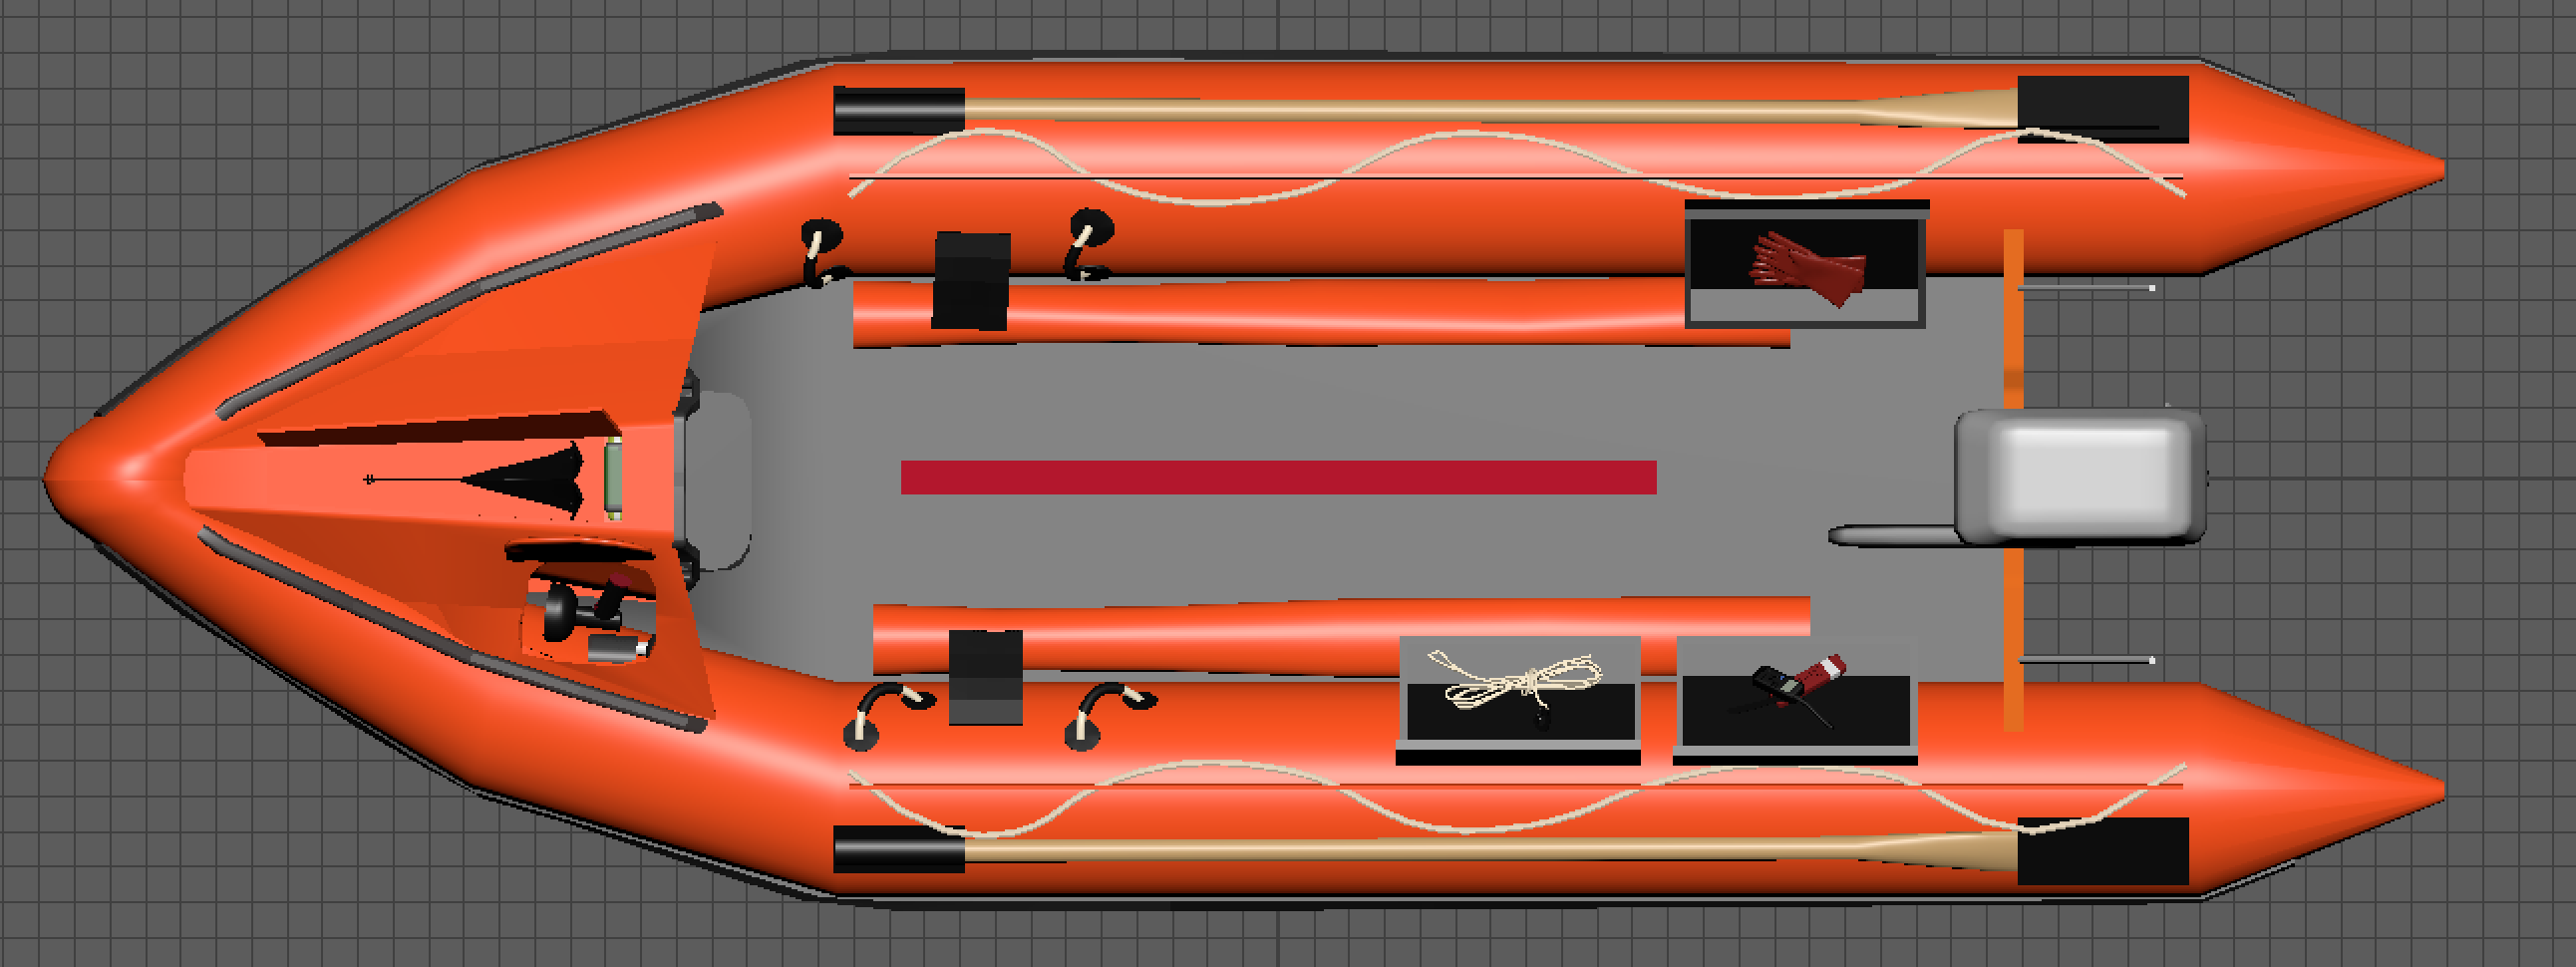
\includegraphics[width=0.6\textwidth]{images/top_model}
\captionof{figure}{Screenshot of final model of D-Class lifeboat}
\label{model}
\hfill \break
\end{minipage}

\subsubsection{Items}
% Add discussion about constructing all nine objects + images of all nine objects
\begin{minipage}{\textwidth}
\begin{center}
    \centering
    \begin{minipage}{0.25\textwidth}
        \centering
        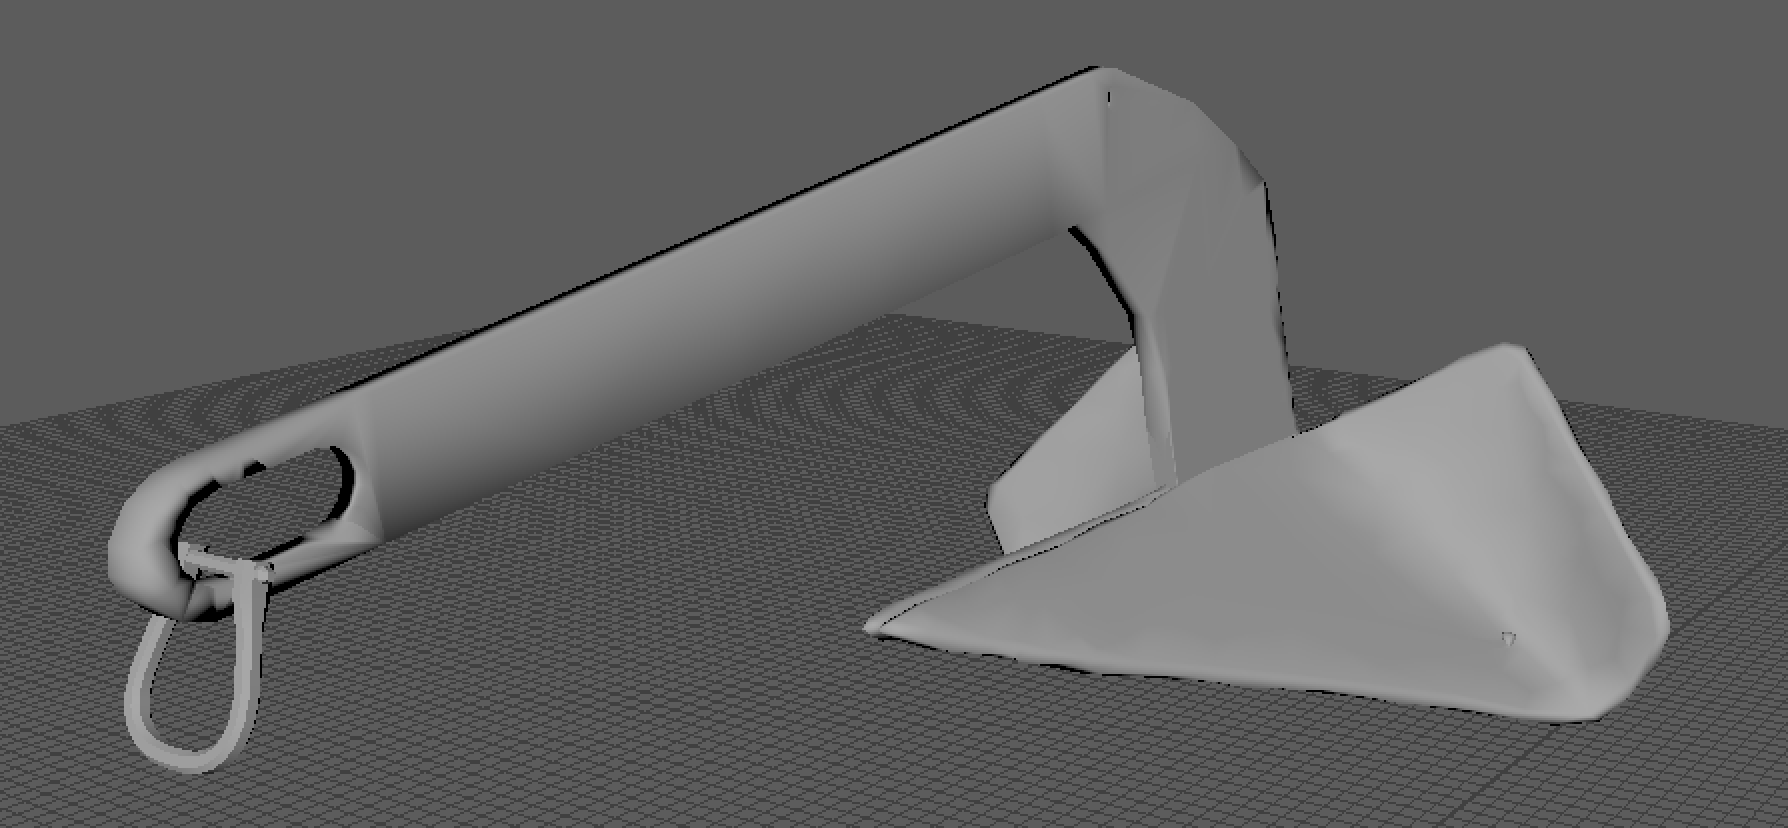
\includegraphics[width=1\textwidth]{images/anchor.png}
    \end{minipage}\hfill
    \begin{minipage}{0.25\textwidth}
        \centering
        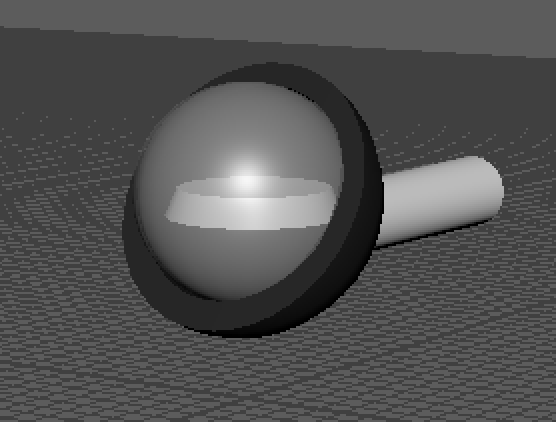
\includegraphics[width=1\textwidth]{images/compass.png}
    \end{minipage}\hfill
    \begin{minipage}{0.25\textwidth}
        \centering
        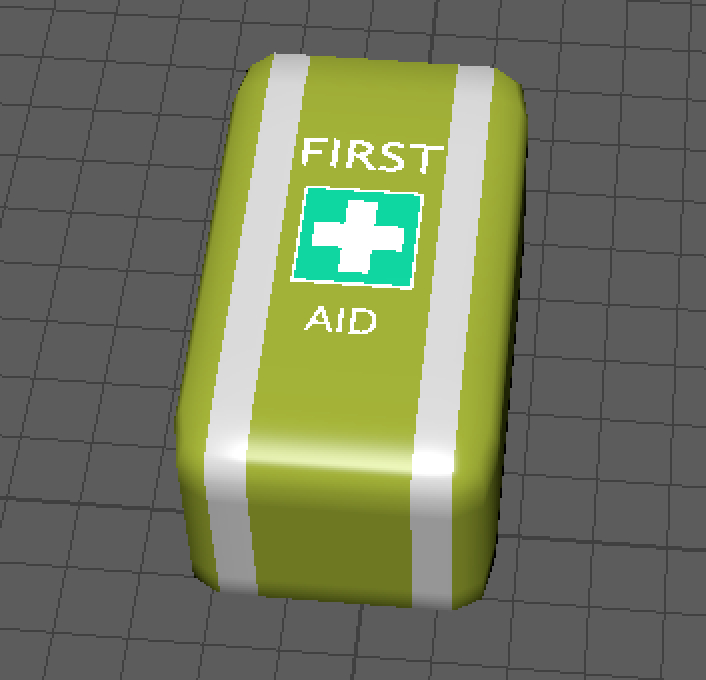
\includegraphics[width=1\textwidth]{images/firstaid.png}
    \end{minipage}\hfill
\end{center}
\begin{center}
    \centering
    \begin{minipage}{0.25\textwidth}
        \centering
        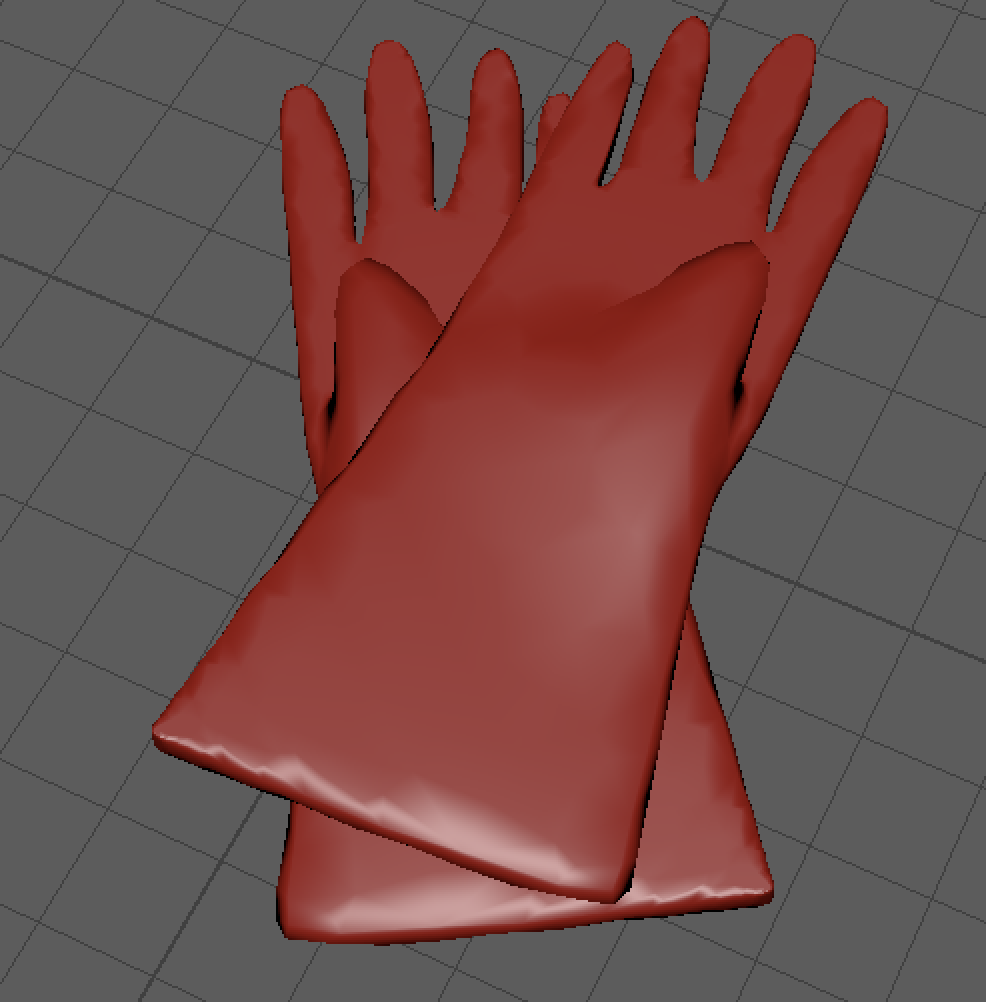
\includegraphics[width=1\textwidth]{images/gloves.png}
    \end{minipage}\hfill
    \begin{minipage}{0.25\textwidth}
        \centering
        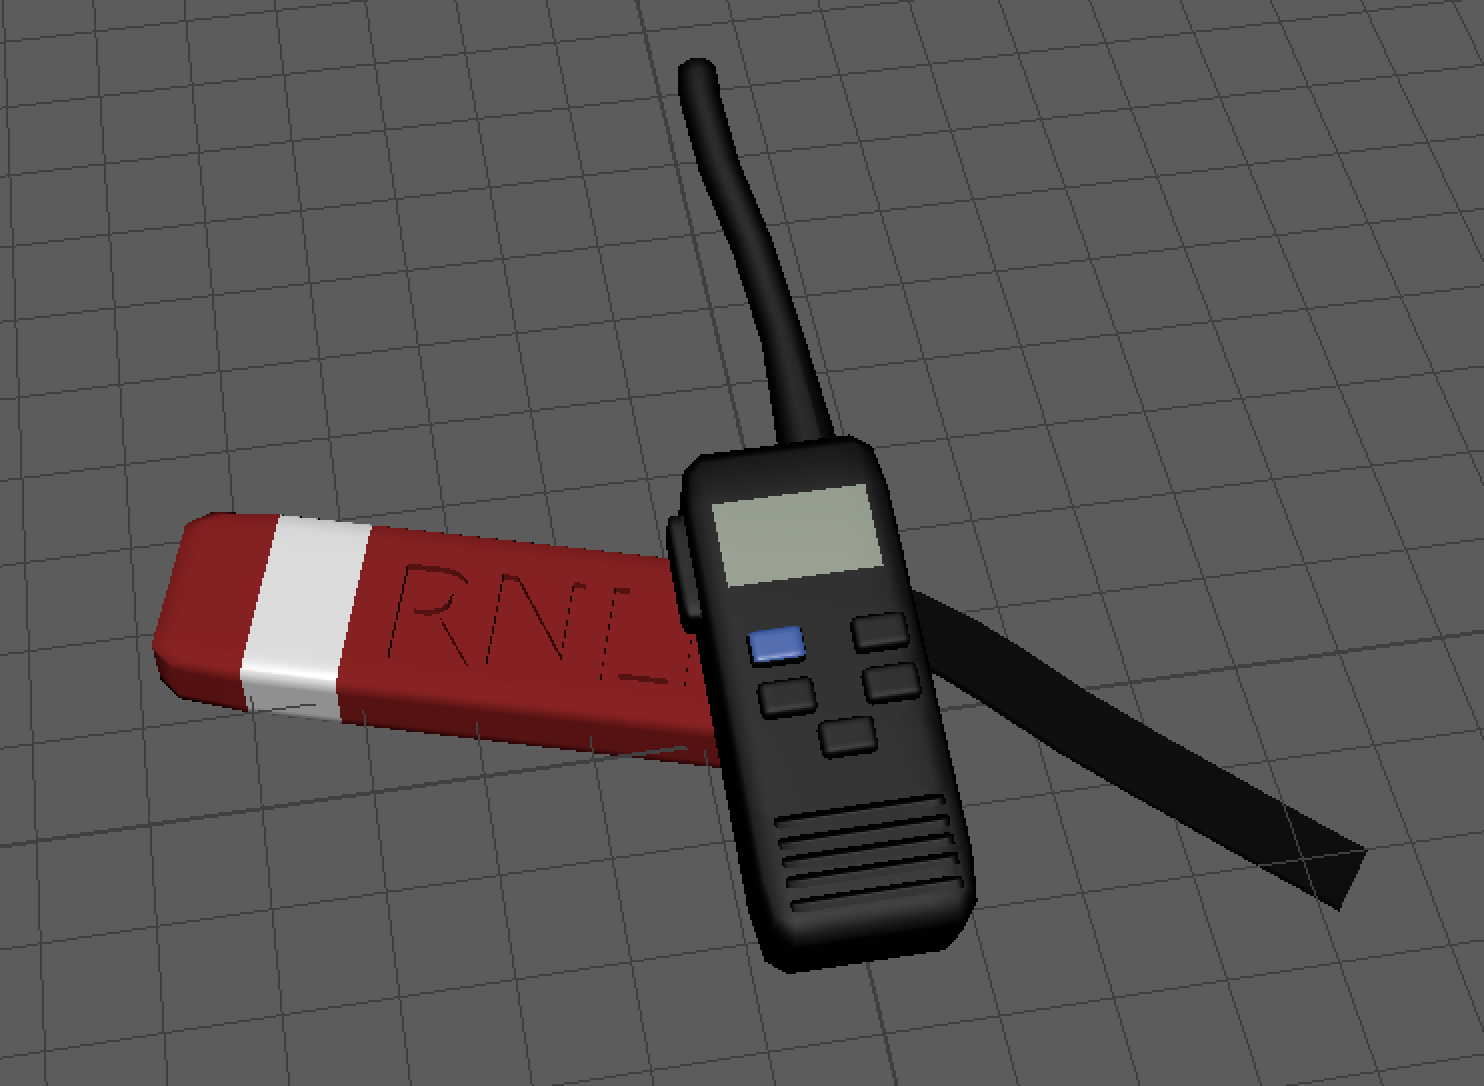
\includegraphics[width=1\textwidth]{images/handheld.png}
    \end{minipage}\hfill
    \begin{minipage}{0.25\textwidth}
        \centering
        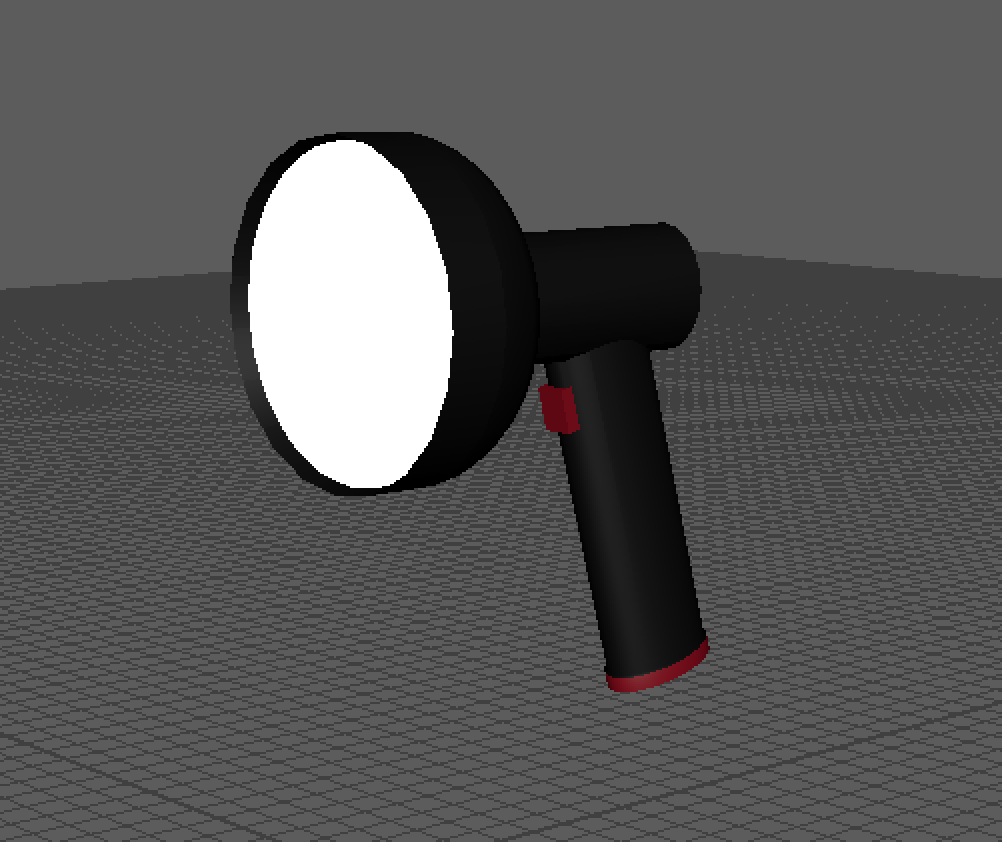
\includegraphics[width=1\textwidth]{images/light.png}
    \end{minipage}\hfill
\end{center}
\begin{center}
    \centering
    \begin{minipage}{0.25\textwidth}
        \centering
        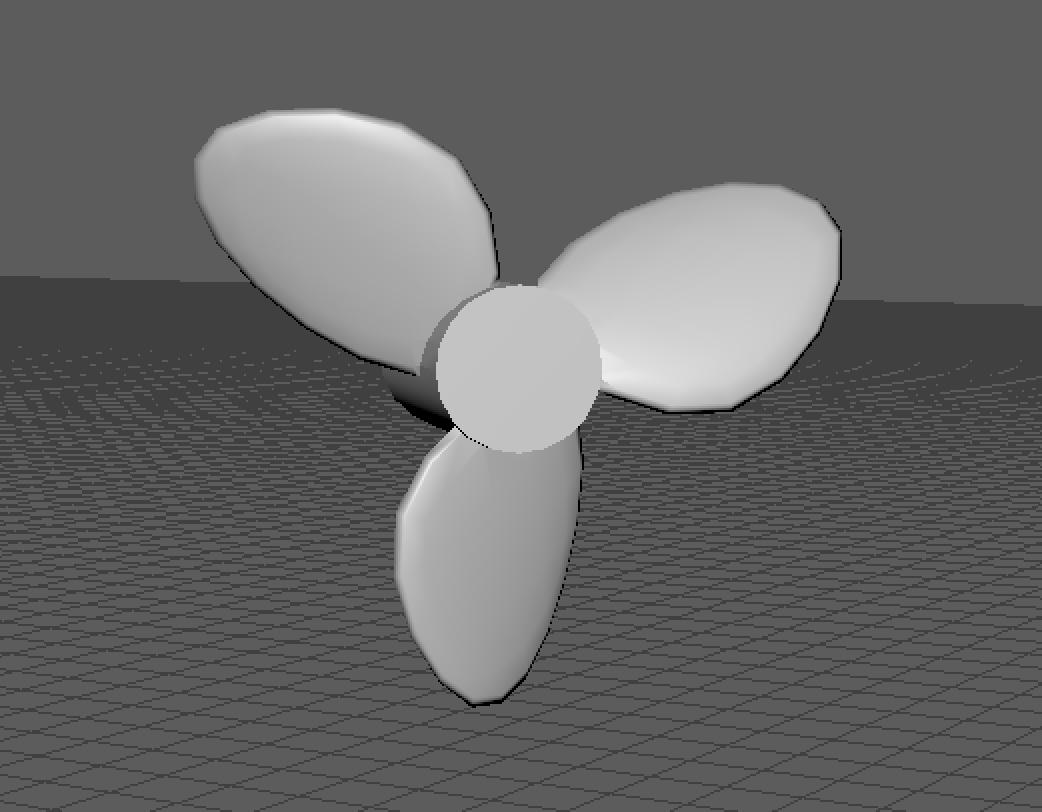
\includegraphics[width=1\textwidth]{images/prop.png}
    \end{minipage}\hfill
    \begin{minipage}{0.25\textwidth}
        \centering
        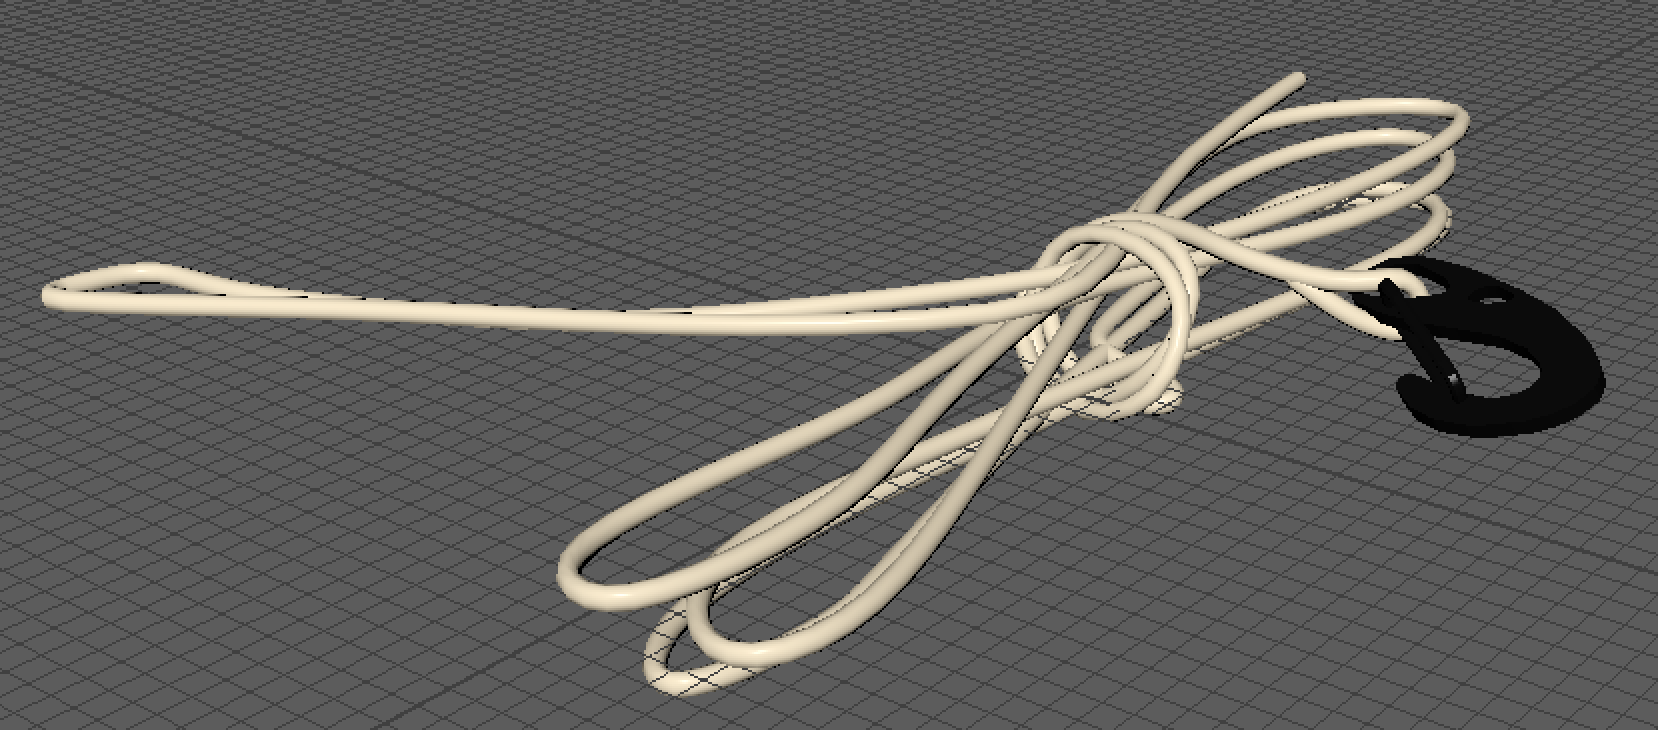
\includegraphics[width=1\textwidth]{images/tow.png}
    \end{minipage}\hfill
    \begin{minipage}{0.25\textwidth}
        \centering
        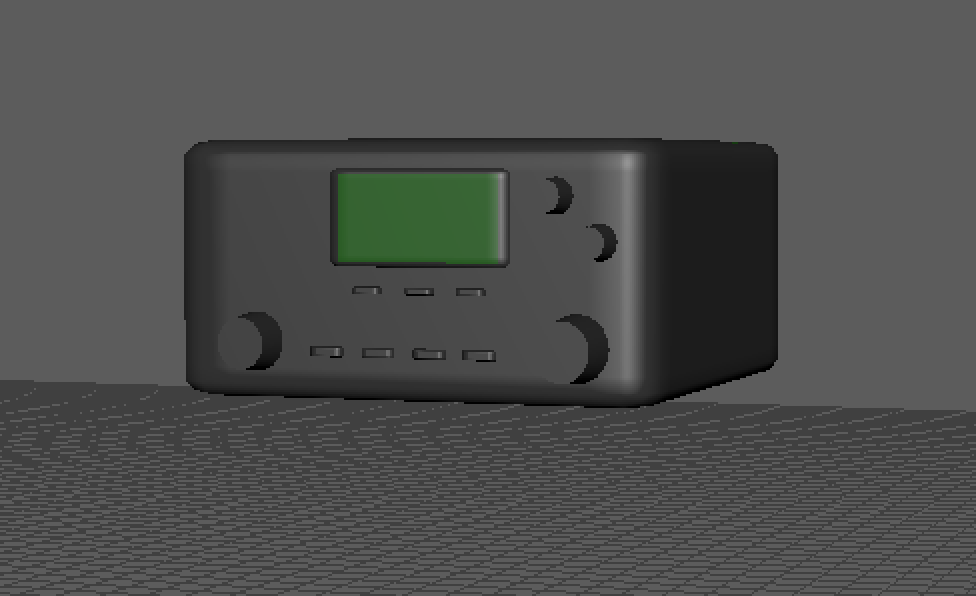
\includegraphics[width=1\textwidth]{images/vhf.png}
    \end{minipage}\hfill
\end{center}
\captionof{figure}{3D models of the nine items that each user would be required to recall}
\end{minipage}

Each item is modelled using the same method of tracing over an image plane. The images that are traced over are the images that are used in the 360-environment. This ensures that there is little variation between the environments for how recognisable each object is. 

The intricacy of some of these models means that it was not easy to use the simple polygonal primitives which are offered by Maya. Instead, the more sophisticated curves, and NURB surfaces needed to be used. Once constructed, these can be converted into polygonal meshes automatically by Maya, and then imported into the model of the entire vessel. In particular, the gloves required this technique. 

\subsubsection{Gloves}
Using Maya's powerful tools effectively can make formerly complex tasks much more manageable. In this case, Maya's curves, and NURB surfaces allows a user to create complex geometry quickly. The process for constructing the gloves item is as follows: 

\begin{itemize}
    \item Create CV curve outlining the desired shape
    \item Create a planar surface from this curve
    \item Convert the surface to a polygon
    \item Add divisions to smooth
\end{itemize}

This workflow is illustrated in Figure \ref{gloves}

\begin{minipage}{\textwidth}
    \begin{center}
    \centering
    \begin{minipage}{0.18\textwidth}
        \centering
        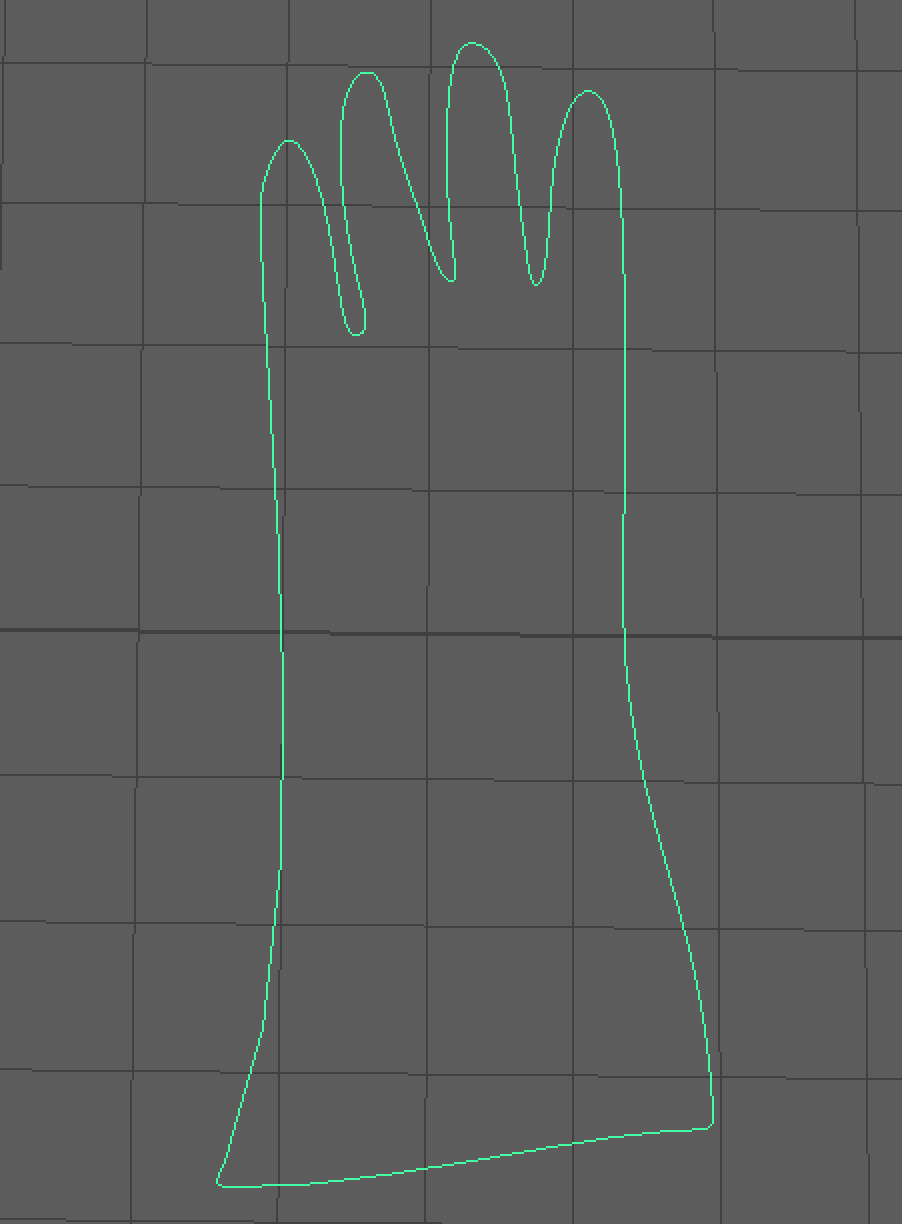
\includegraphics[width=1\textwidth]{images/curve.png}
    \end{minipage}\hfill
    \begin{minipage}{0.18\textwidth}
        \centering
        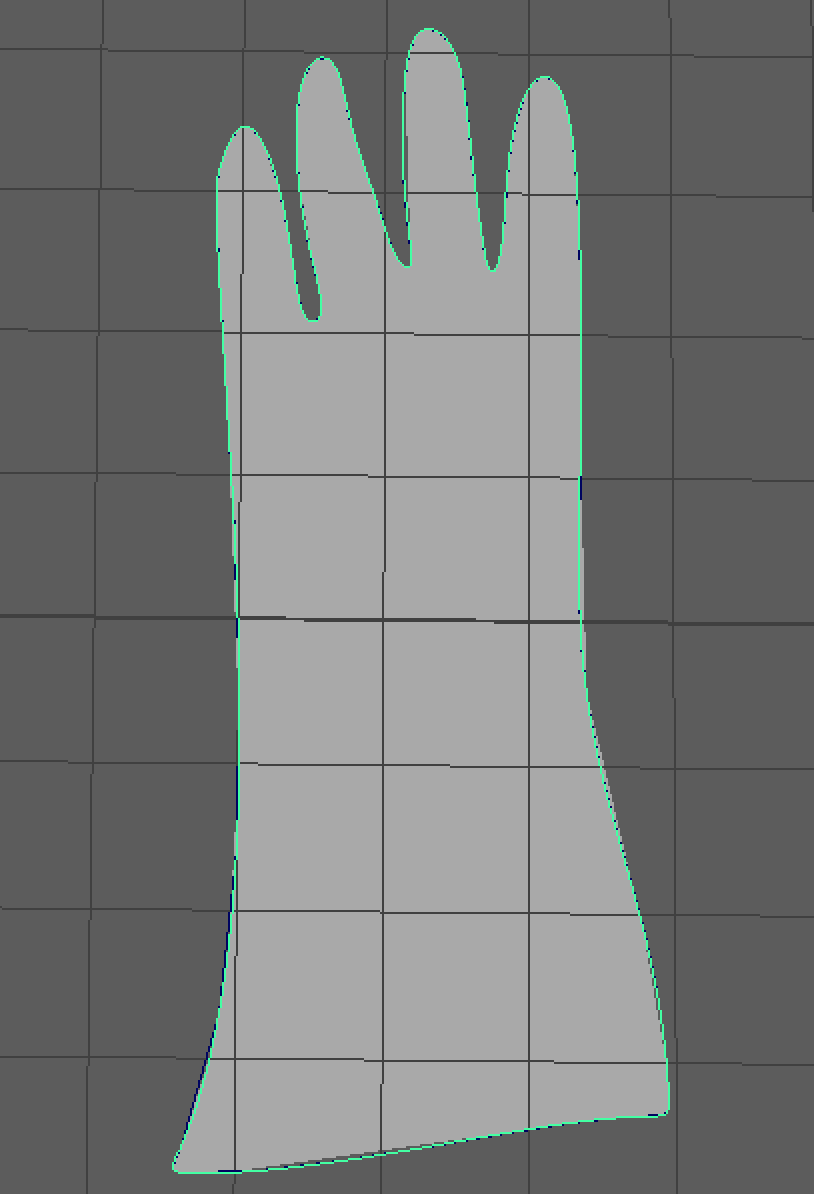
\includegraphics[width=1\textwidth]{images/planar.png}
    \end{minipage}\hfill
    \begin{minipage}{0.18\textwidth}
        \centering
        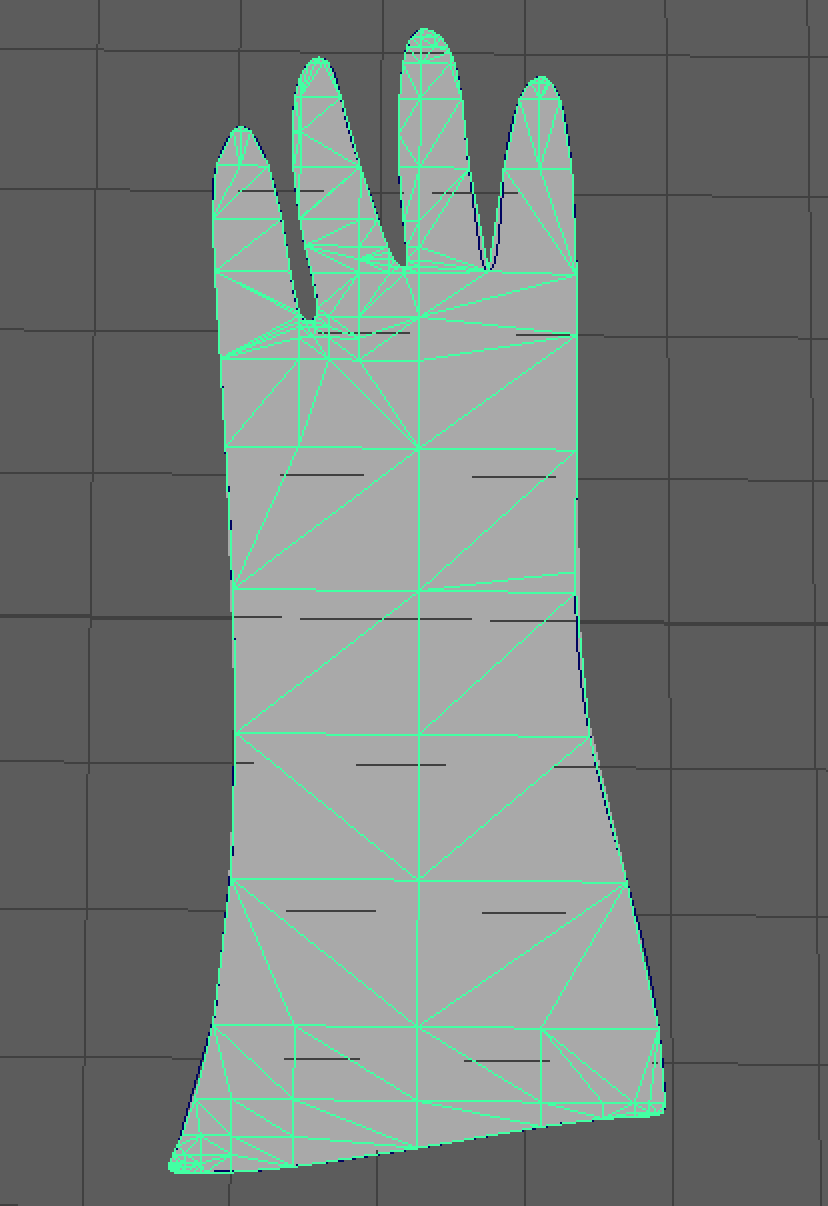
\includegraphics[width=1\textwidth]{images/topoly.png}
    \end{minipage}\hfill
        \centering
    \begin{minipage}{0.18\textwidth}
        \centering
        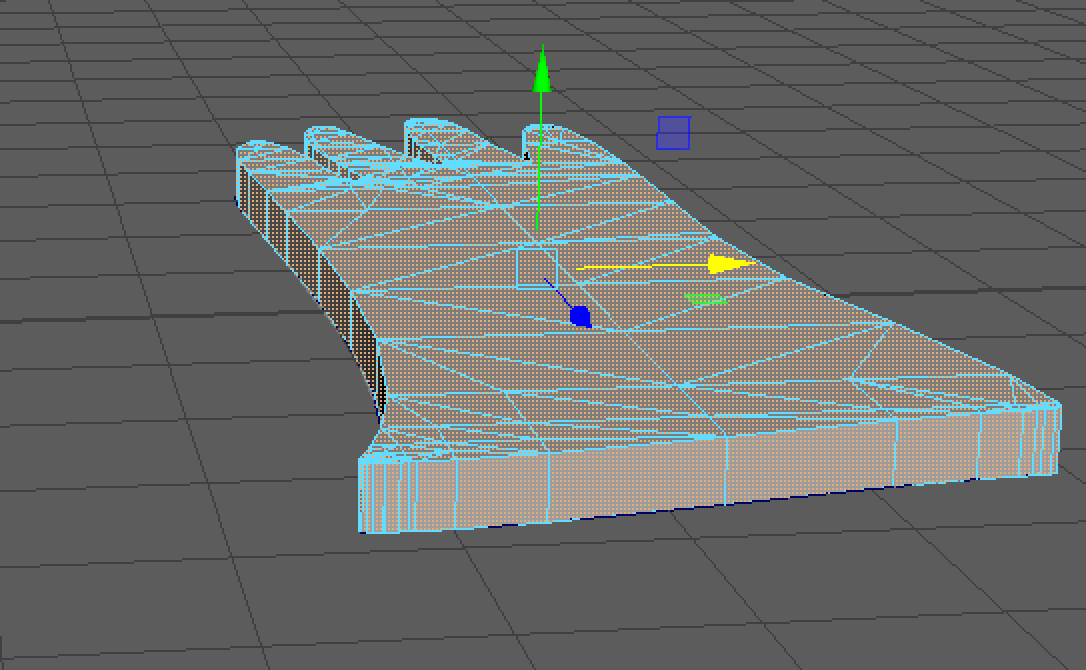
\includegraphics[width=1\textwidth]{images/extrude.png}
    \end{minipage}\hfill
    \begin{minipage}{0.18\textwidth}
        \centering
        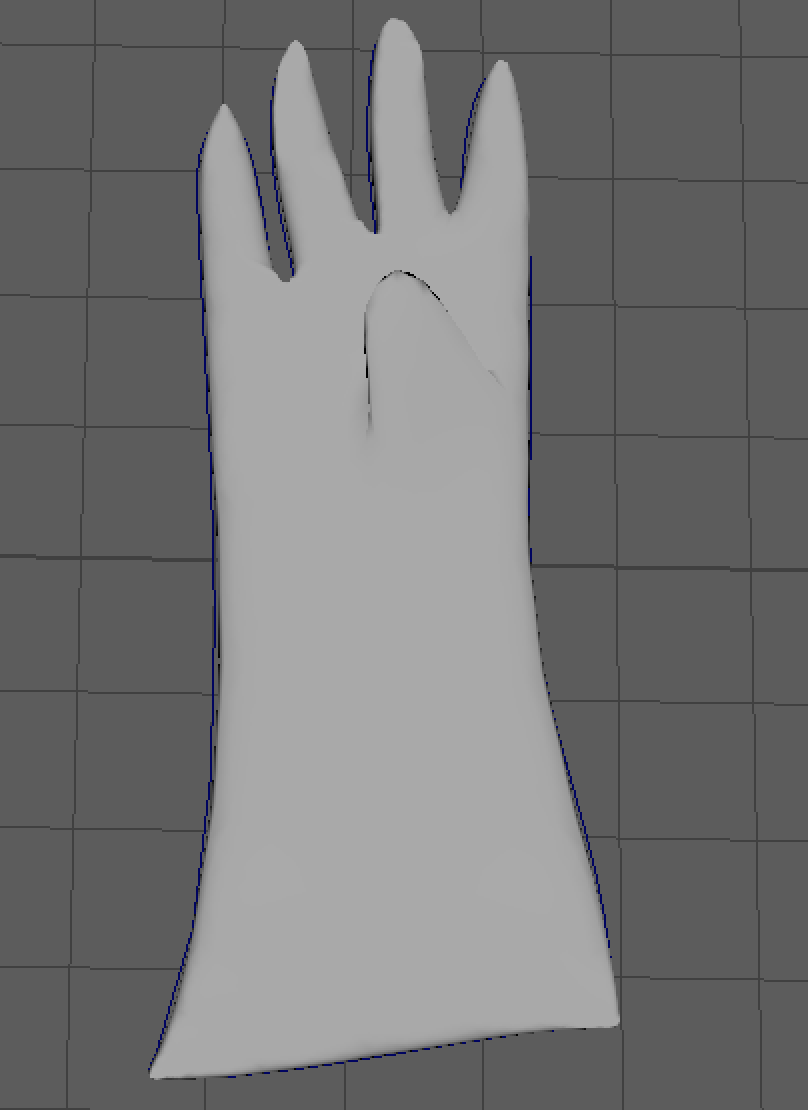
\includegraphics[width=1\textwidth]{images/adddivision.png}
    \end{minipage}\hfill
\end{center}
\captionof{figure}{Workflow used to construct the 3D model of the gloves item.}
\label{gloves}
\end{minipage}

\subsubsection{Tow Rope}
Another task that would have otherwise been complex was the construction of the tow rope model. An intricate spool of rope would be almost impossible to model manually. Soft selection is a tool which assisted in this, soft selection allows a user to select a vertex, edge, or face, then when moving that item nearby items are affected relative to the change of that item and their distance from it. The process for this model was: 

\begin{itemize}
    \item Construct 2D curve by tracing image plane of object
    \item Position polygonal face at the end of the curve
    \item Use soft selection, with a radius which extends the length of the rope, to add a third dimension to the model
    \item Add divisions to smooth
\end{itemize}

These steps are illustrated in Figure \ref{tow}

\begin{minipage}{\textwidth}
\centering
\begin{center}
    \centering
    \begin{minipage}{0.18\textwidth}
        \centering
        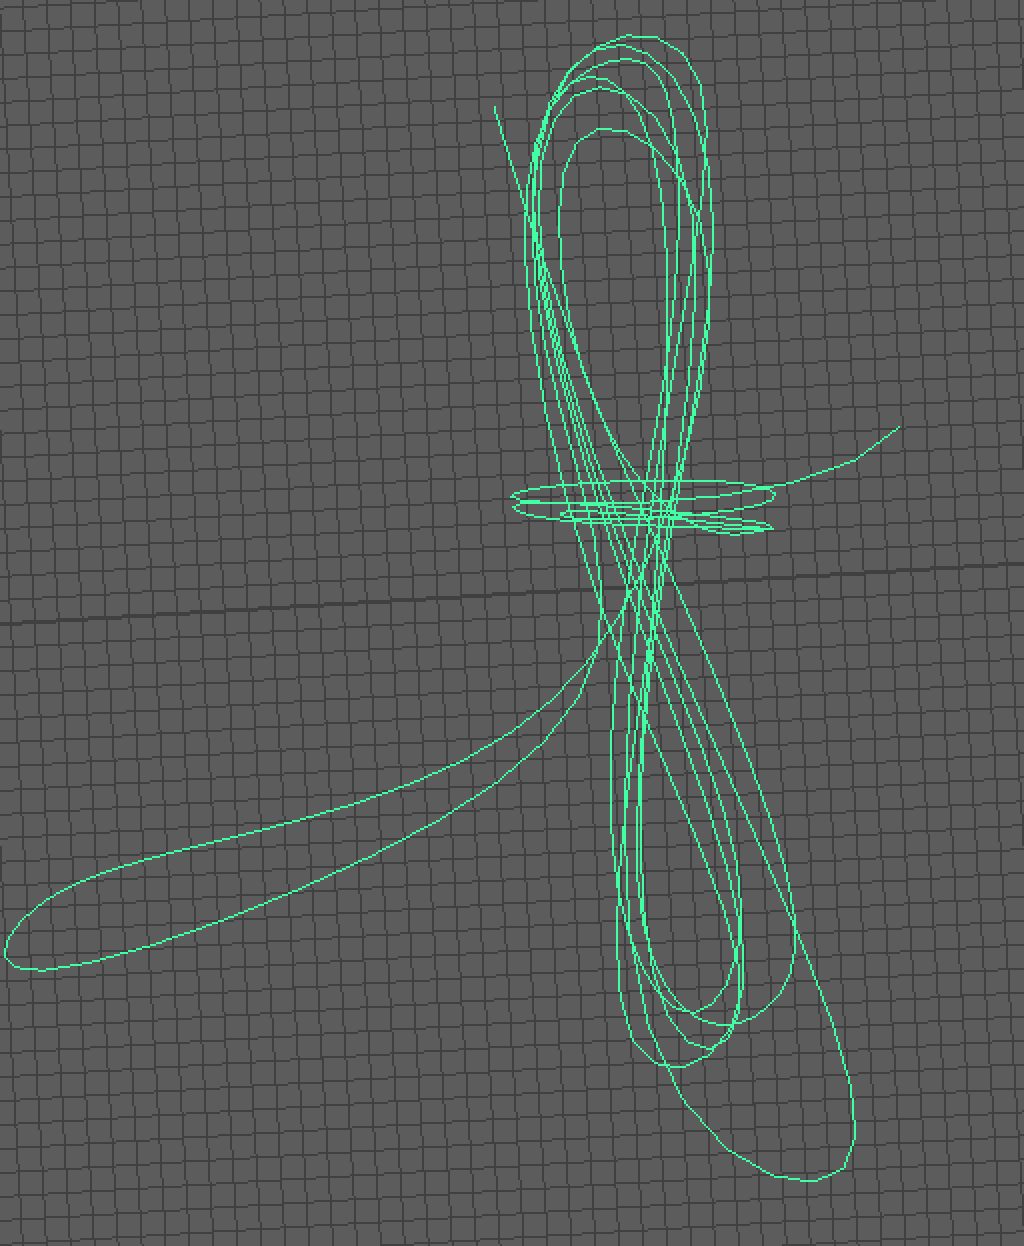
\includegraphics[width=1\textwidth]{images/towcurve.png}
    \end{minipage}\hfill
    \begin{minipage}{0.18\textwidth}
        \centering
        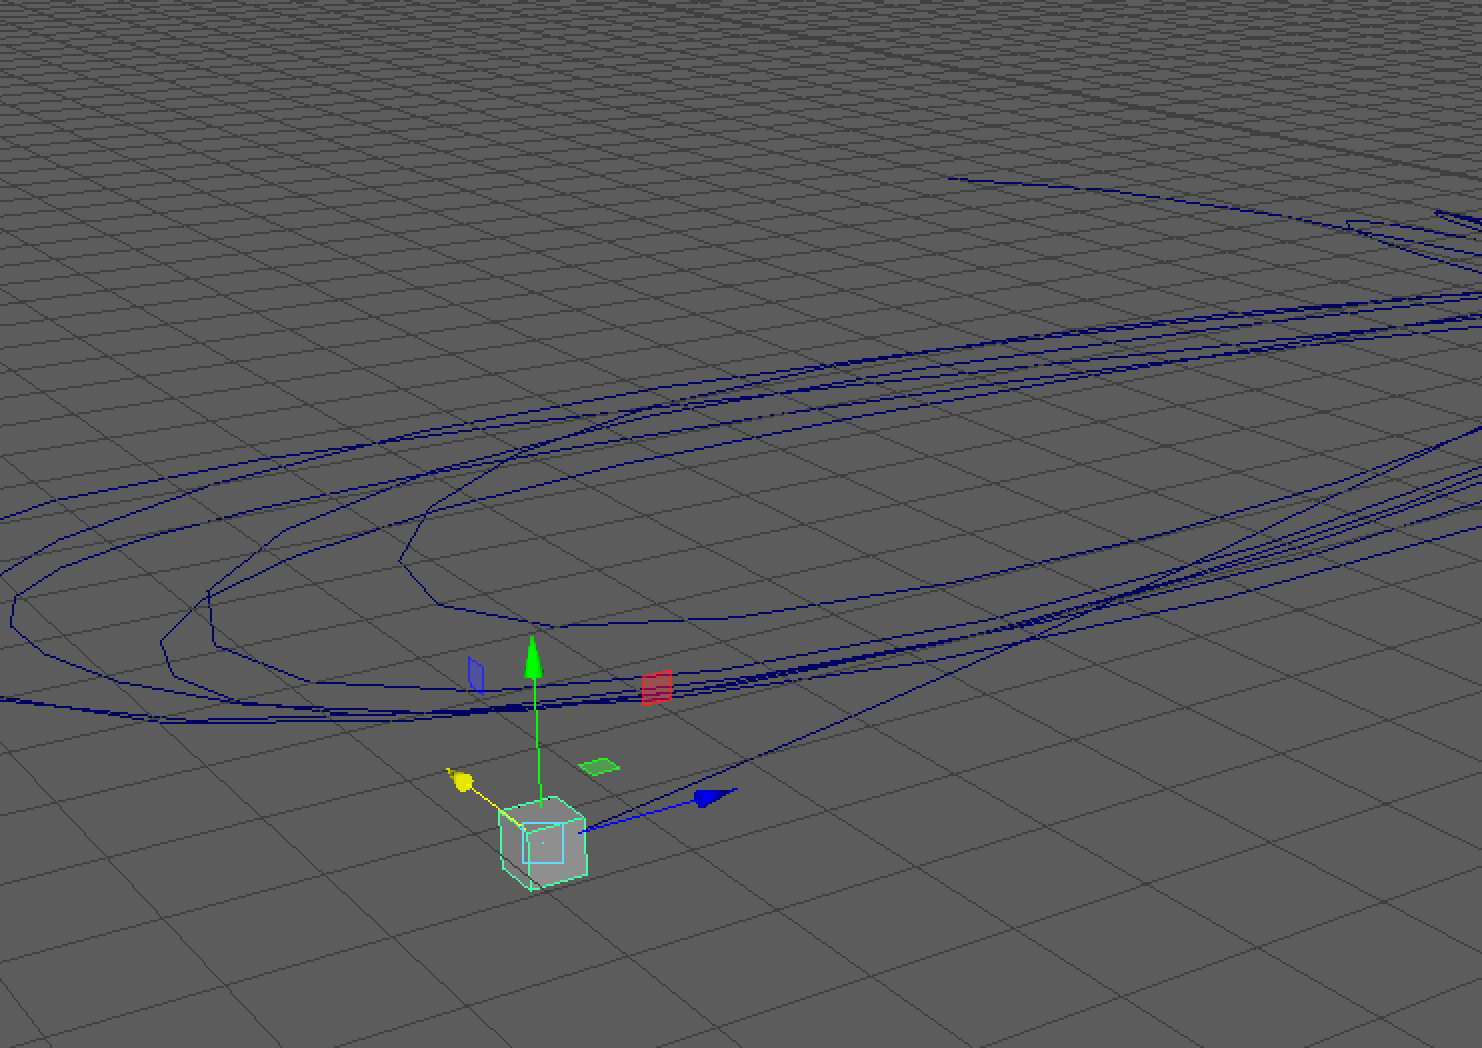
\includegraphics[width=1\textwidth]{images/towpoly.png}
    \end{minipage}\hfill
    \begin{minipage}{0.18\textwidth}
        \centering
        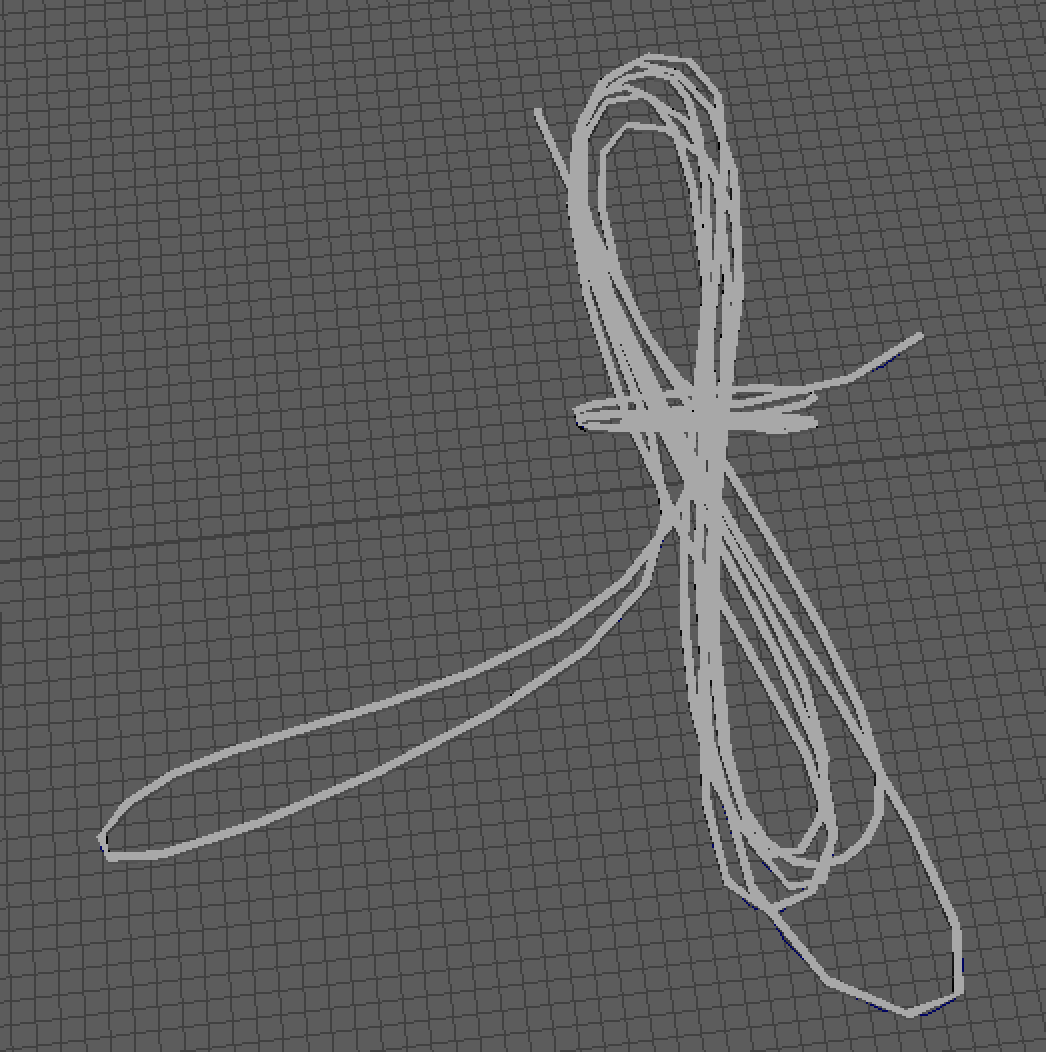
\includegraphics[width=1\textwidth]{images/towextrude.png}
    \end{minipage}\hfill
        \centering
    \begin{minipage}{0.18\textwidth}
        \centering
        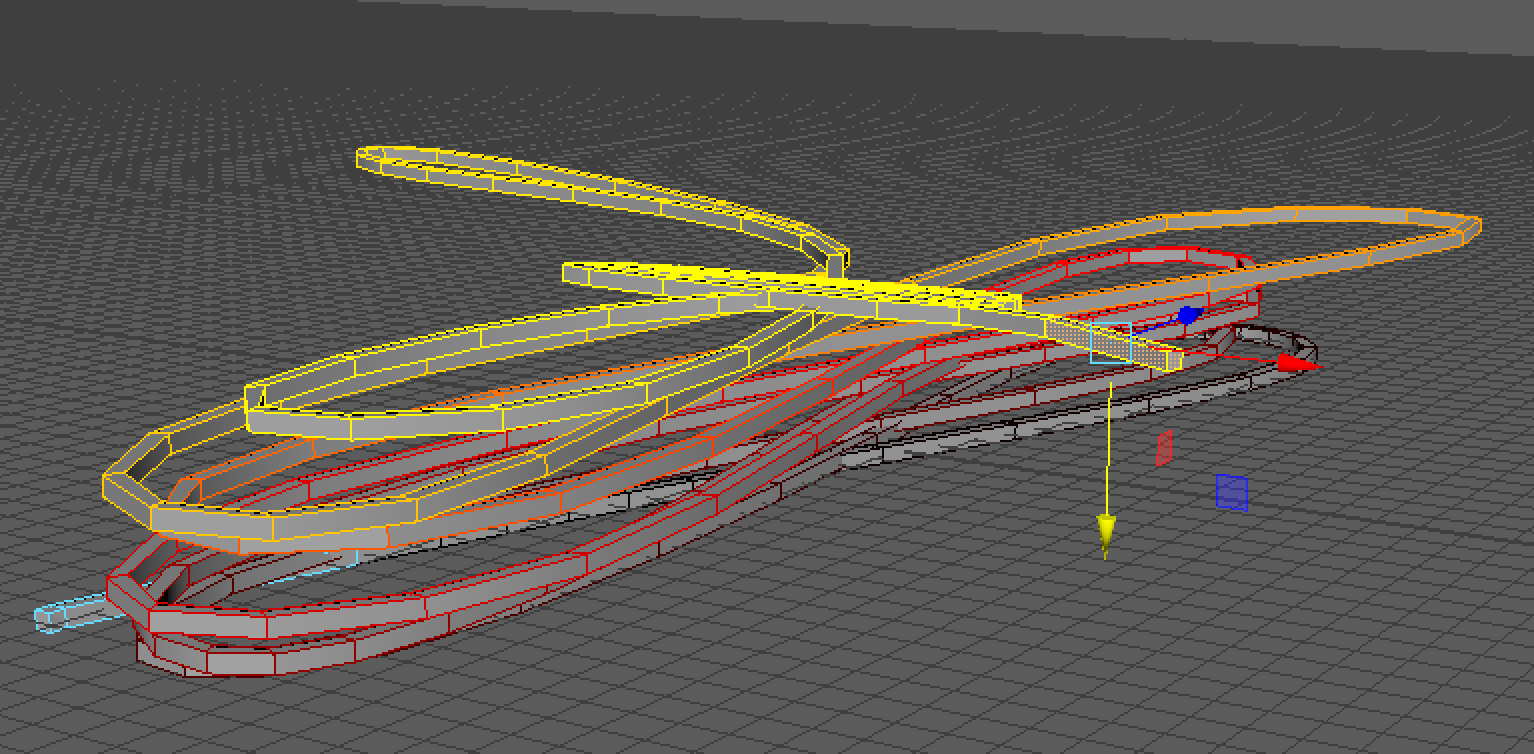
\includegraphics[width=1\textwidth]{images/towsoft.png}
    \end{minipage}\hfill
    \begin{minipage}{0.18\textwidth}
        \centering
        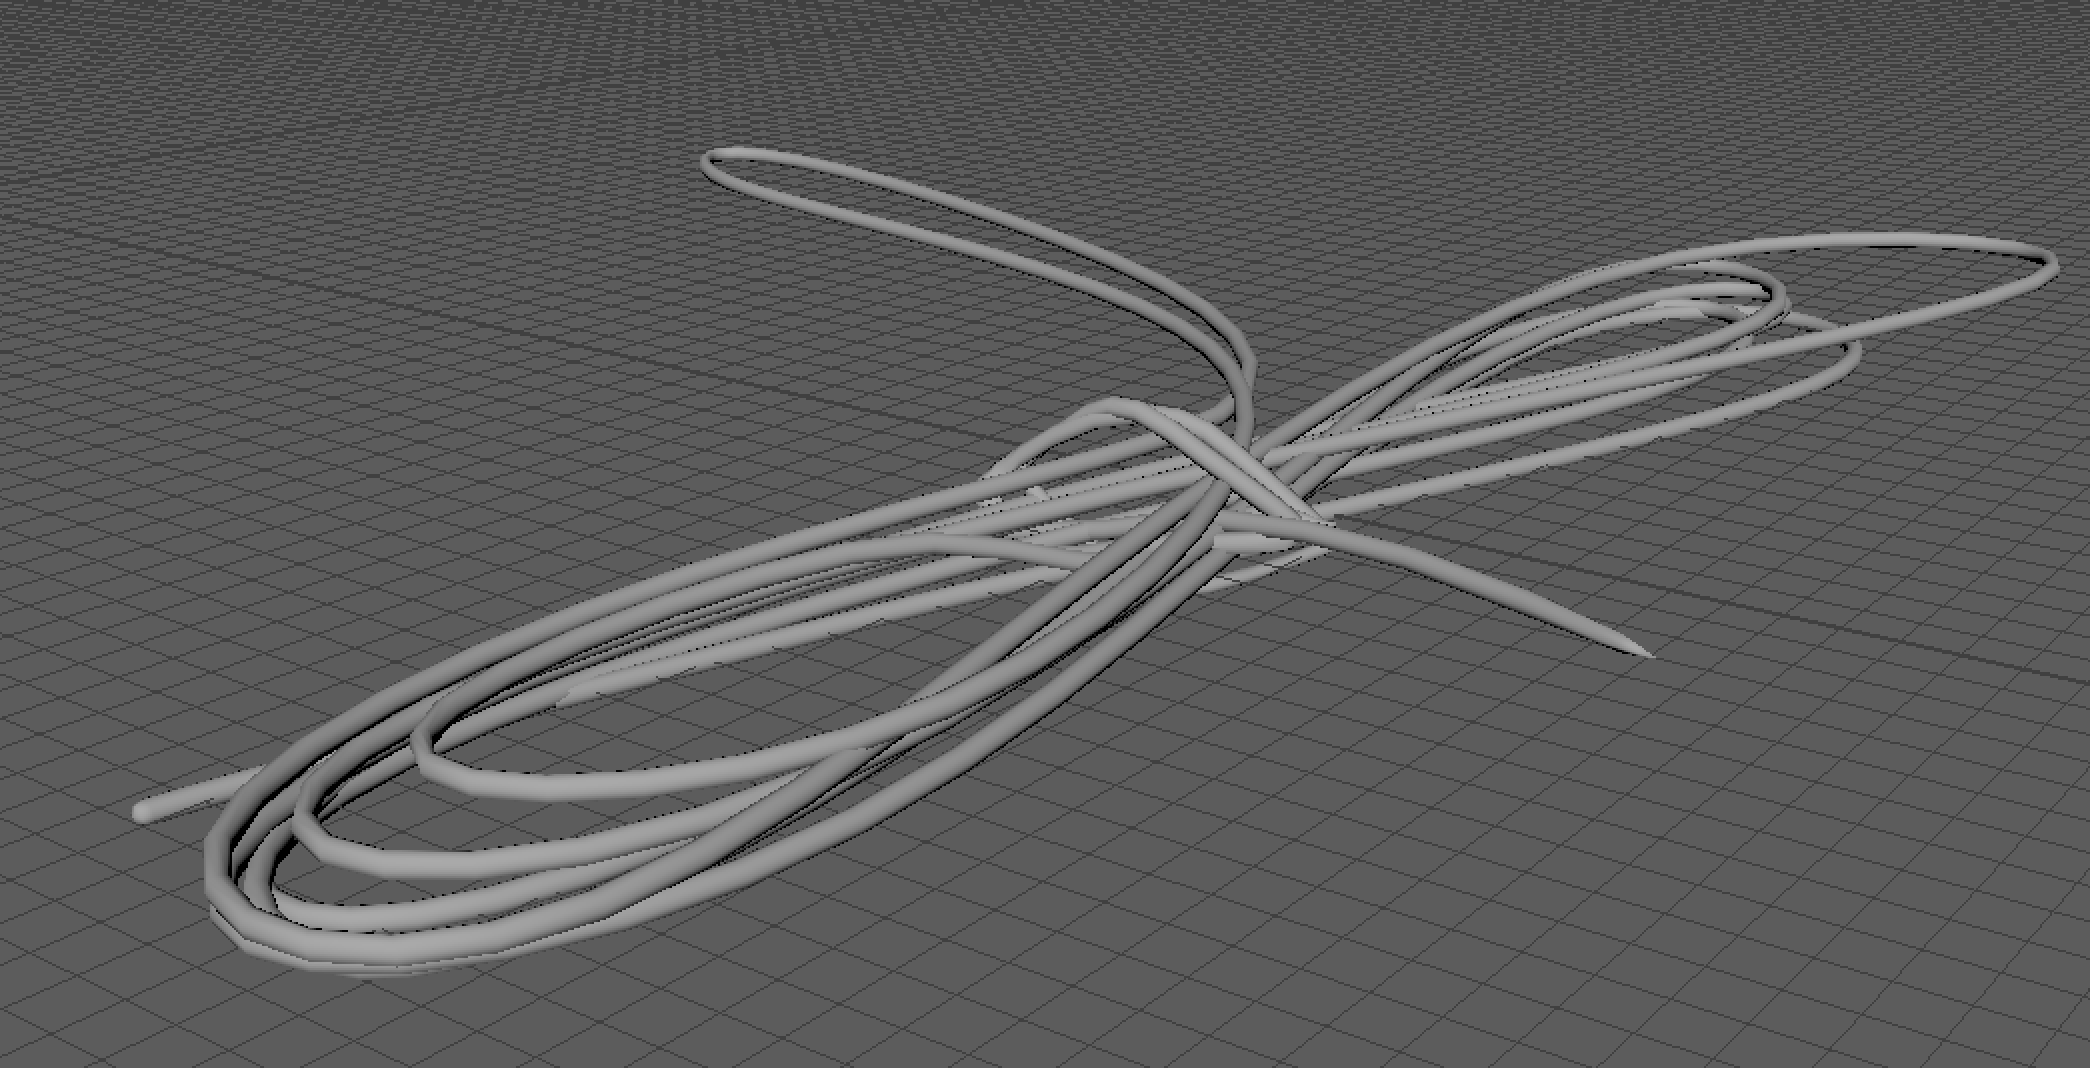
\includegraphics[width=1\textwidth]{images/towdivisions.png}
    \end{minipage}\hfill
\end{center}
\captionof{figure}{Workflow used to construct the 3D model of the tow rope item.}
\label{tow}
\end{minipage}

\subsection{Unity}
Importing the Maya model into Unity is easy. A particularly useful workflow is saving from Maya directly into the Unity assets folder, thus all changes in the Maya file are changed within Unity on save. In order to make the model interact with the environment and to raycasts simple collider primitives are positioned over the model. Although the environment is static, in order for the reticle from the Google Daydream controller to be usable this is a necessity.  

\begin{minipage}{\textwidth}
\hfill \break
\centering
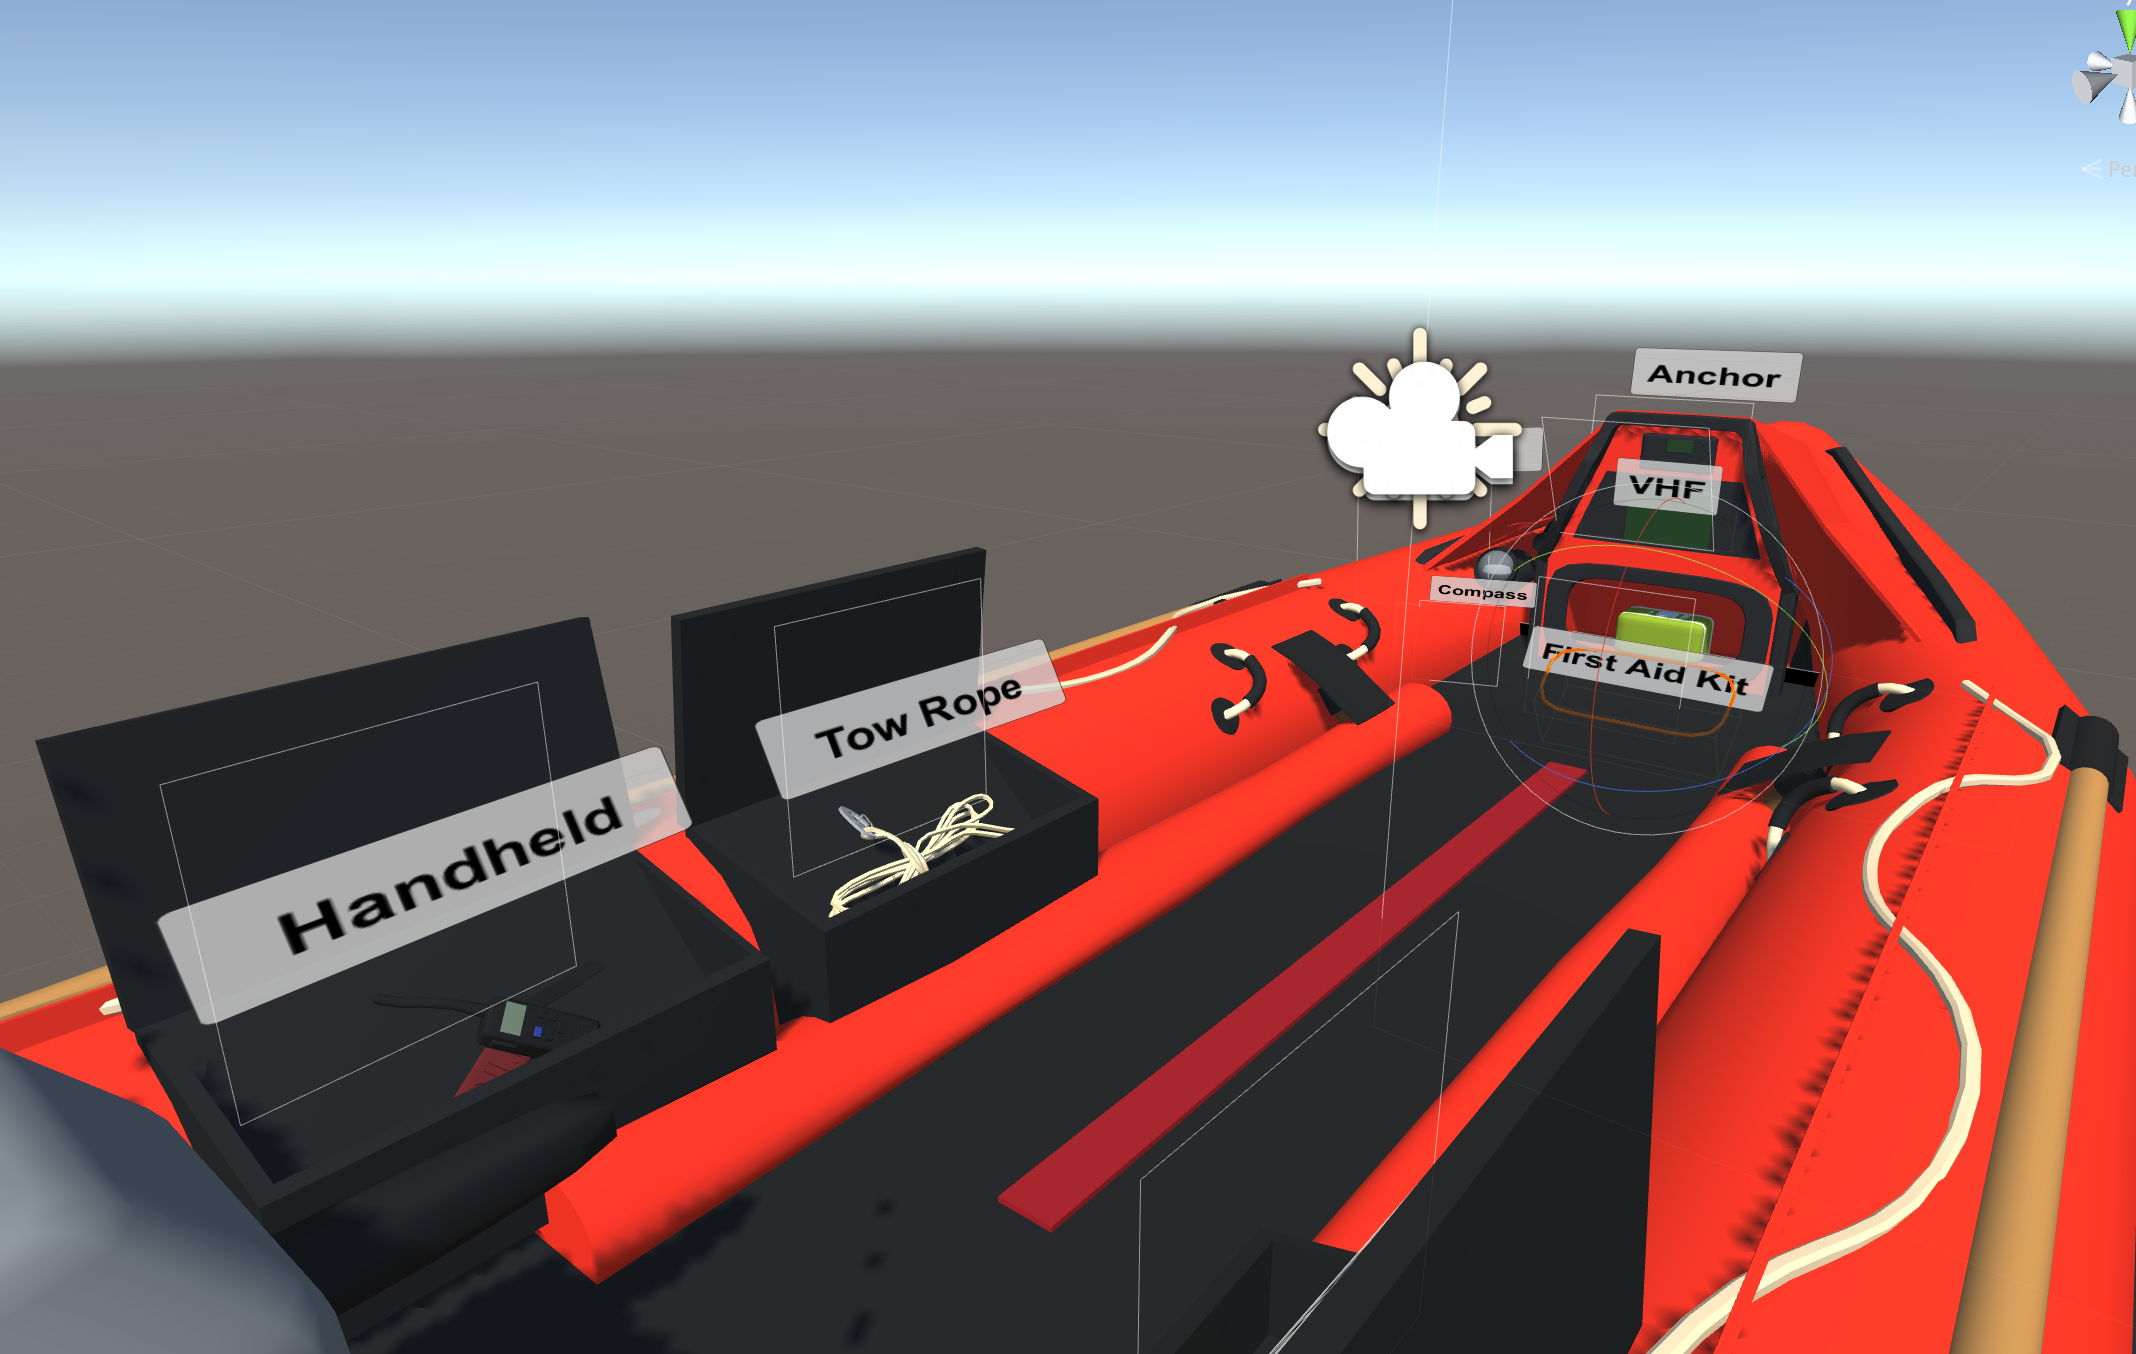
\includegraphics[width=0.6\textwidth]{images/model_unity}
\captionof{figure}{Screenshot of final model of D-Class lifeboat after importing to Unity. UI Labels are also shown.}
\label{model}
\hfill \break
\end{minipage}

\section{360-Image Environment}
The second application which was constructed was an interactive real world environment. This utilises 360-degree images from the actual environment. Users are then able to use the UI elements to explore this environment, and the objects within it. 

\subsection{Samsung Gear 360}
There are many modern cameras which are designed specifically for capturing 360-degree images and video. In this project, the Samsung Gear 360 device was used. Images were captured using a tripod. These images are then imported and stitched using the Gear360 application, and these images are then immediately usable within Unity. An important note to make in order to reduce any need for post processing, is that all images should be taken with the same rotation. This ensures that a users orientation within the environment is consistent throughout exploration; this is demonstrated in Figure \ref{360-items}, notice that each image is almost identical except for the translational movement within the scene. 

\begin{minipage}{\textwidth}
\hfill \break
\centering
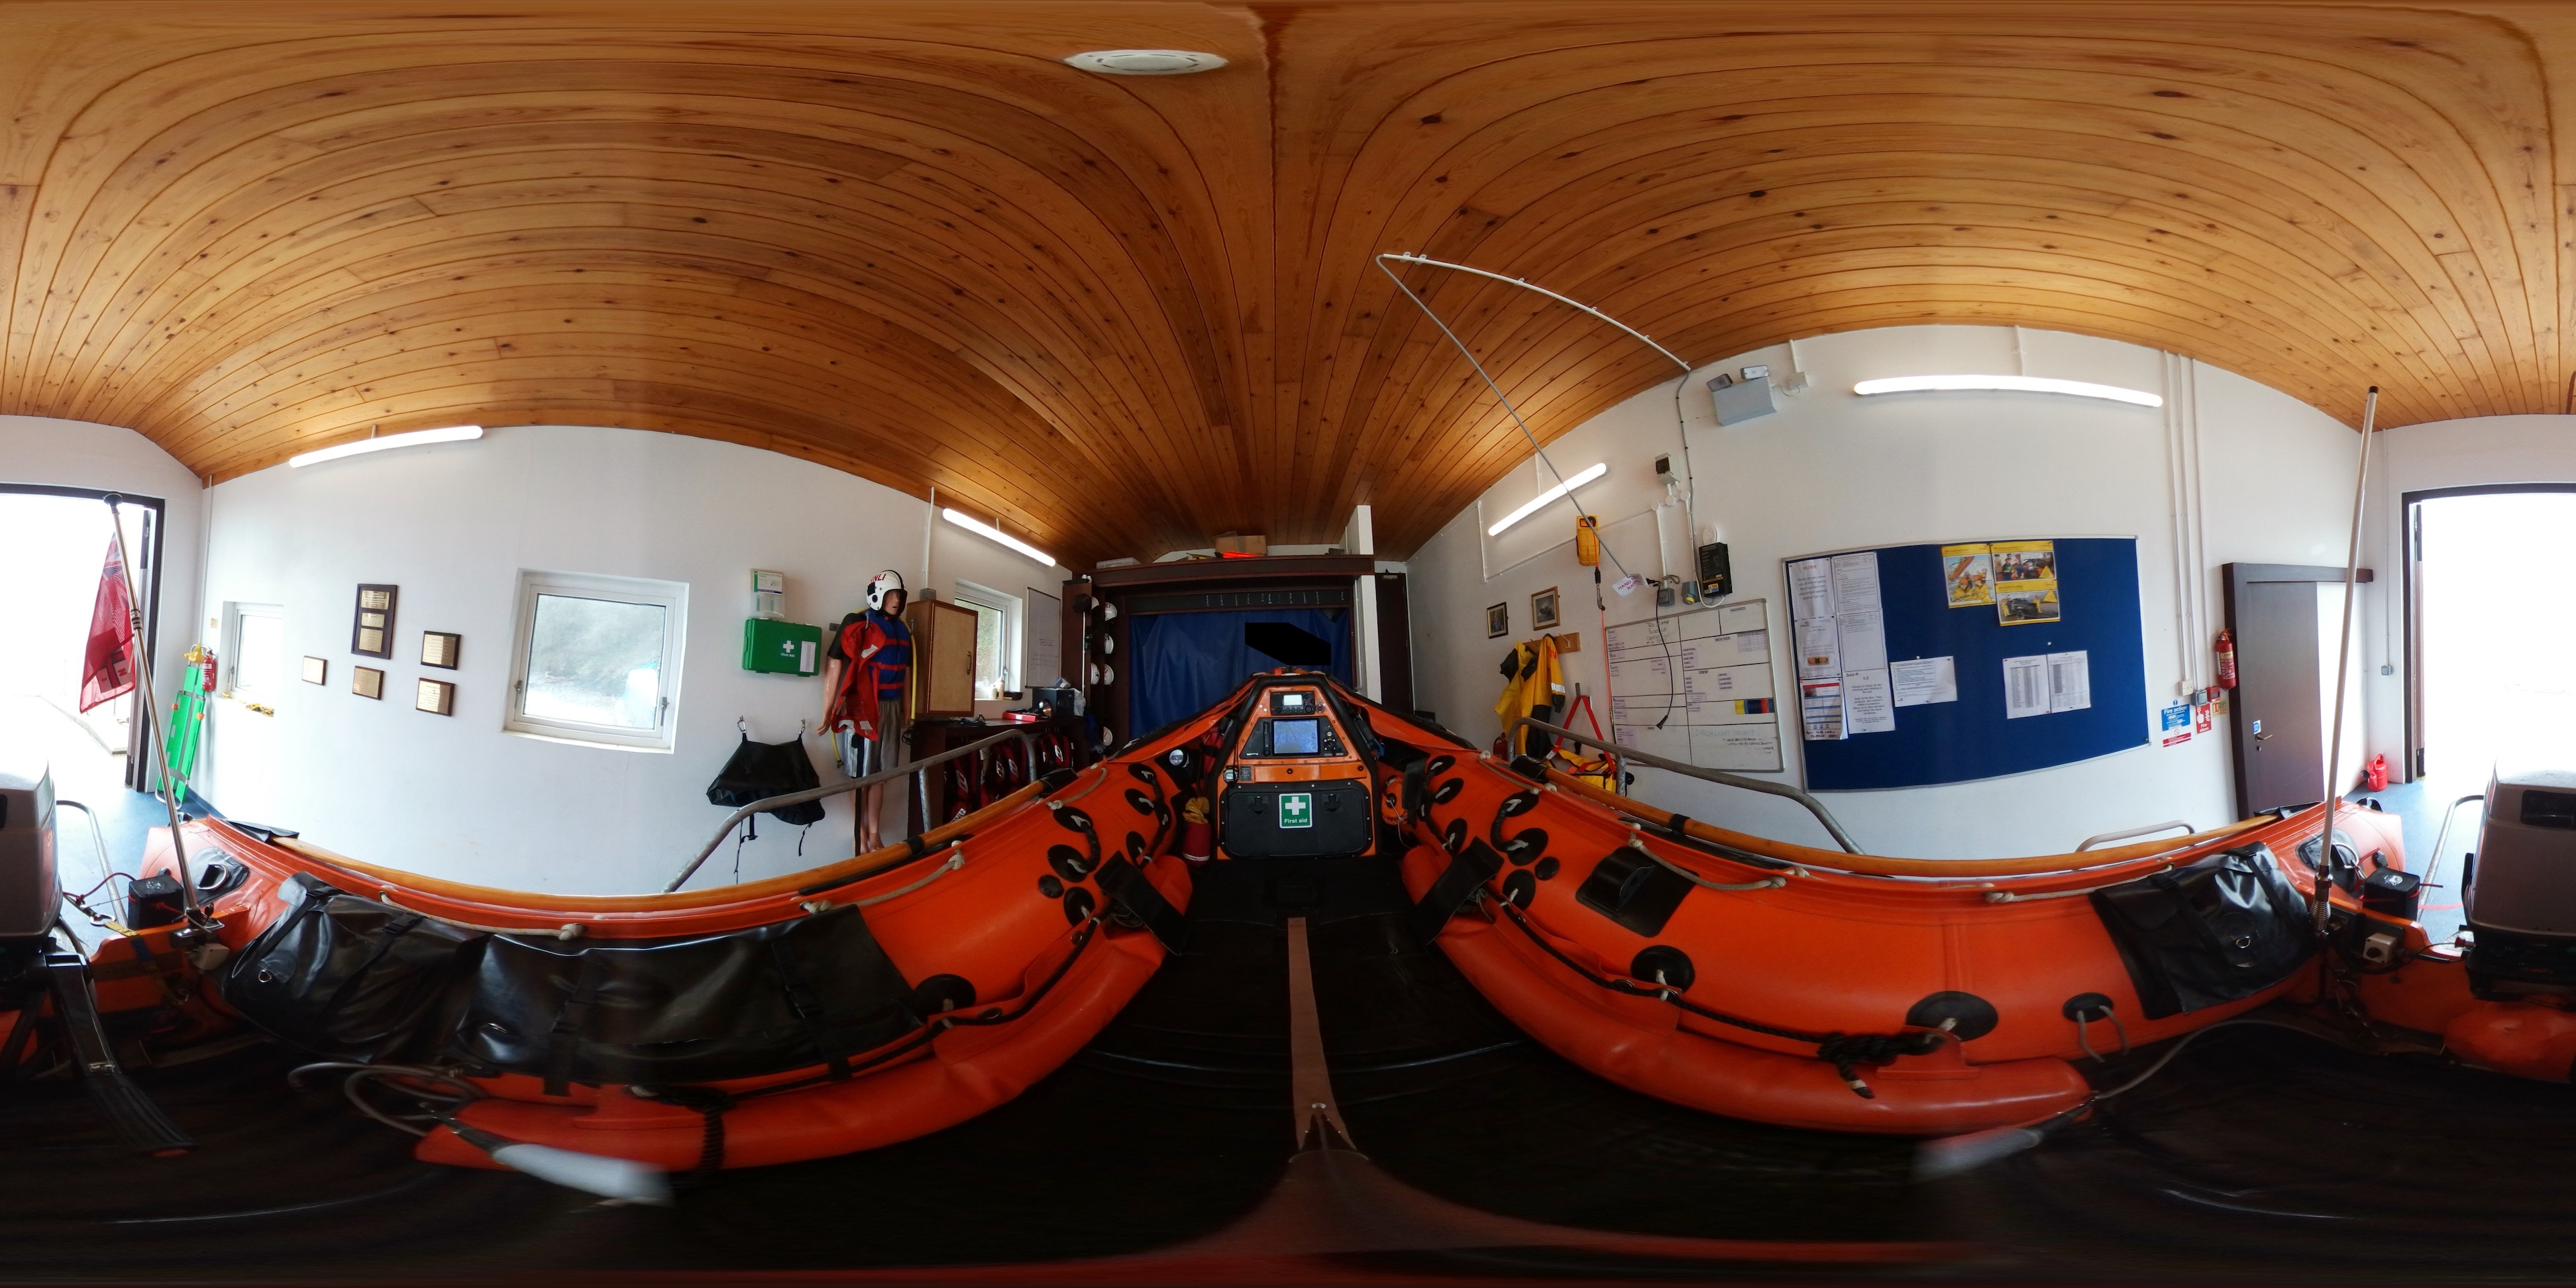
\includegraphics[width=0.8\textwidth]{images/centre}
\captionof{figure}{Image taken on the Samsung Gear 360. This is the Central image used in 360-image environment.}
\label{360-central}
\hfill \break
\end{minipage}

\begin{minipage}{\textwidth}
\begin{center}
    \centering
    \begin{minipage}{0.3\textwidth}
        \centering
        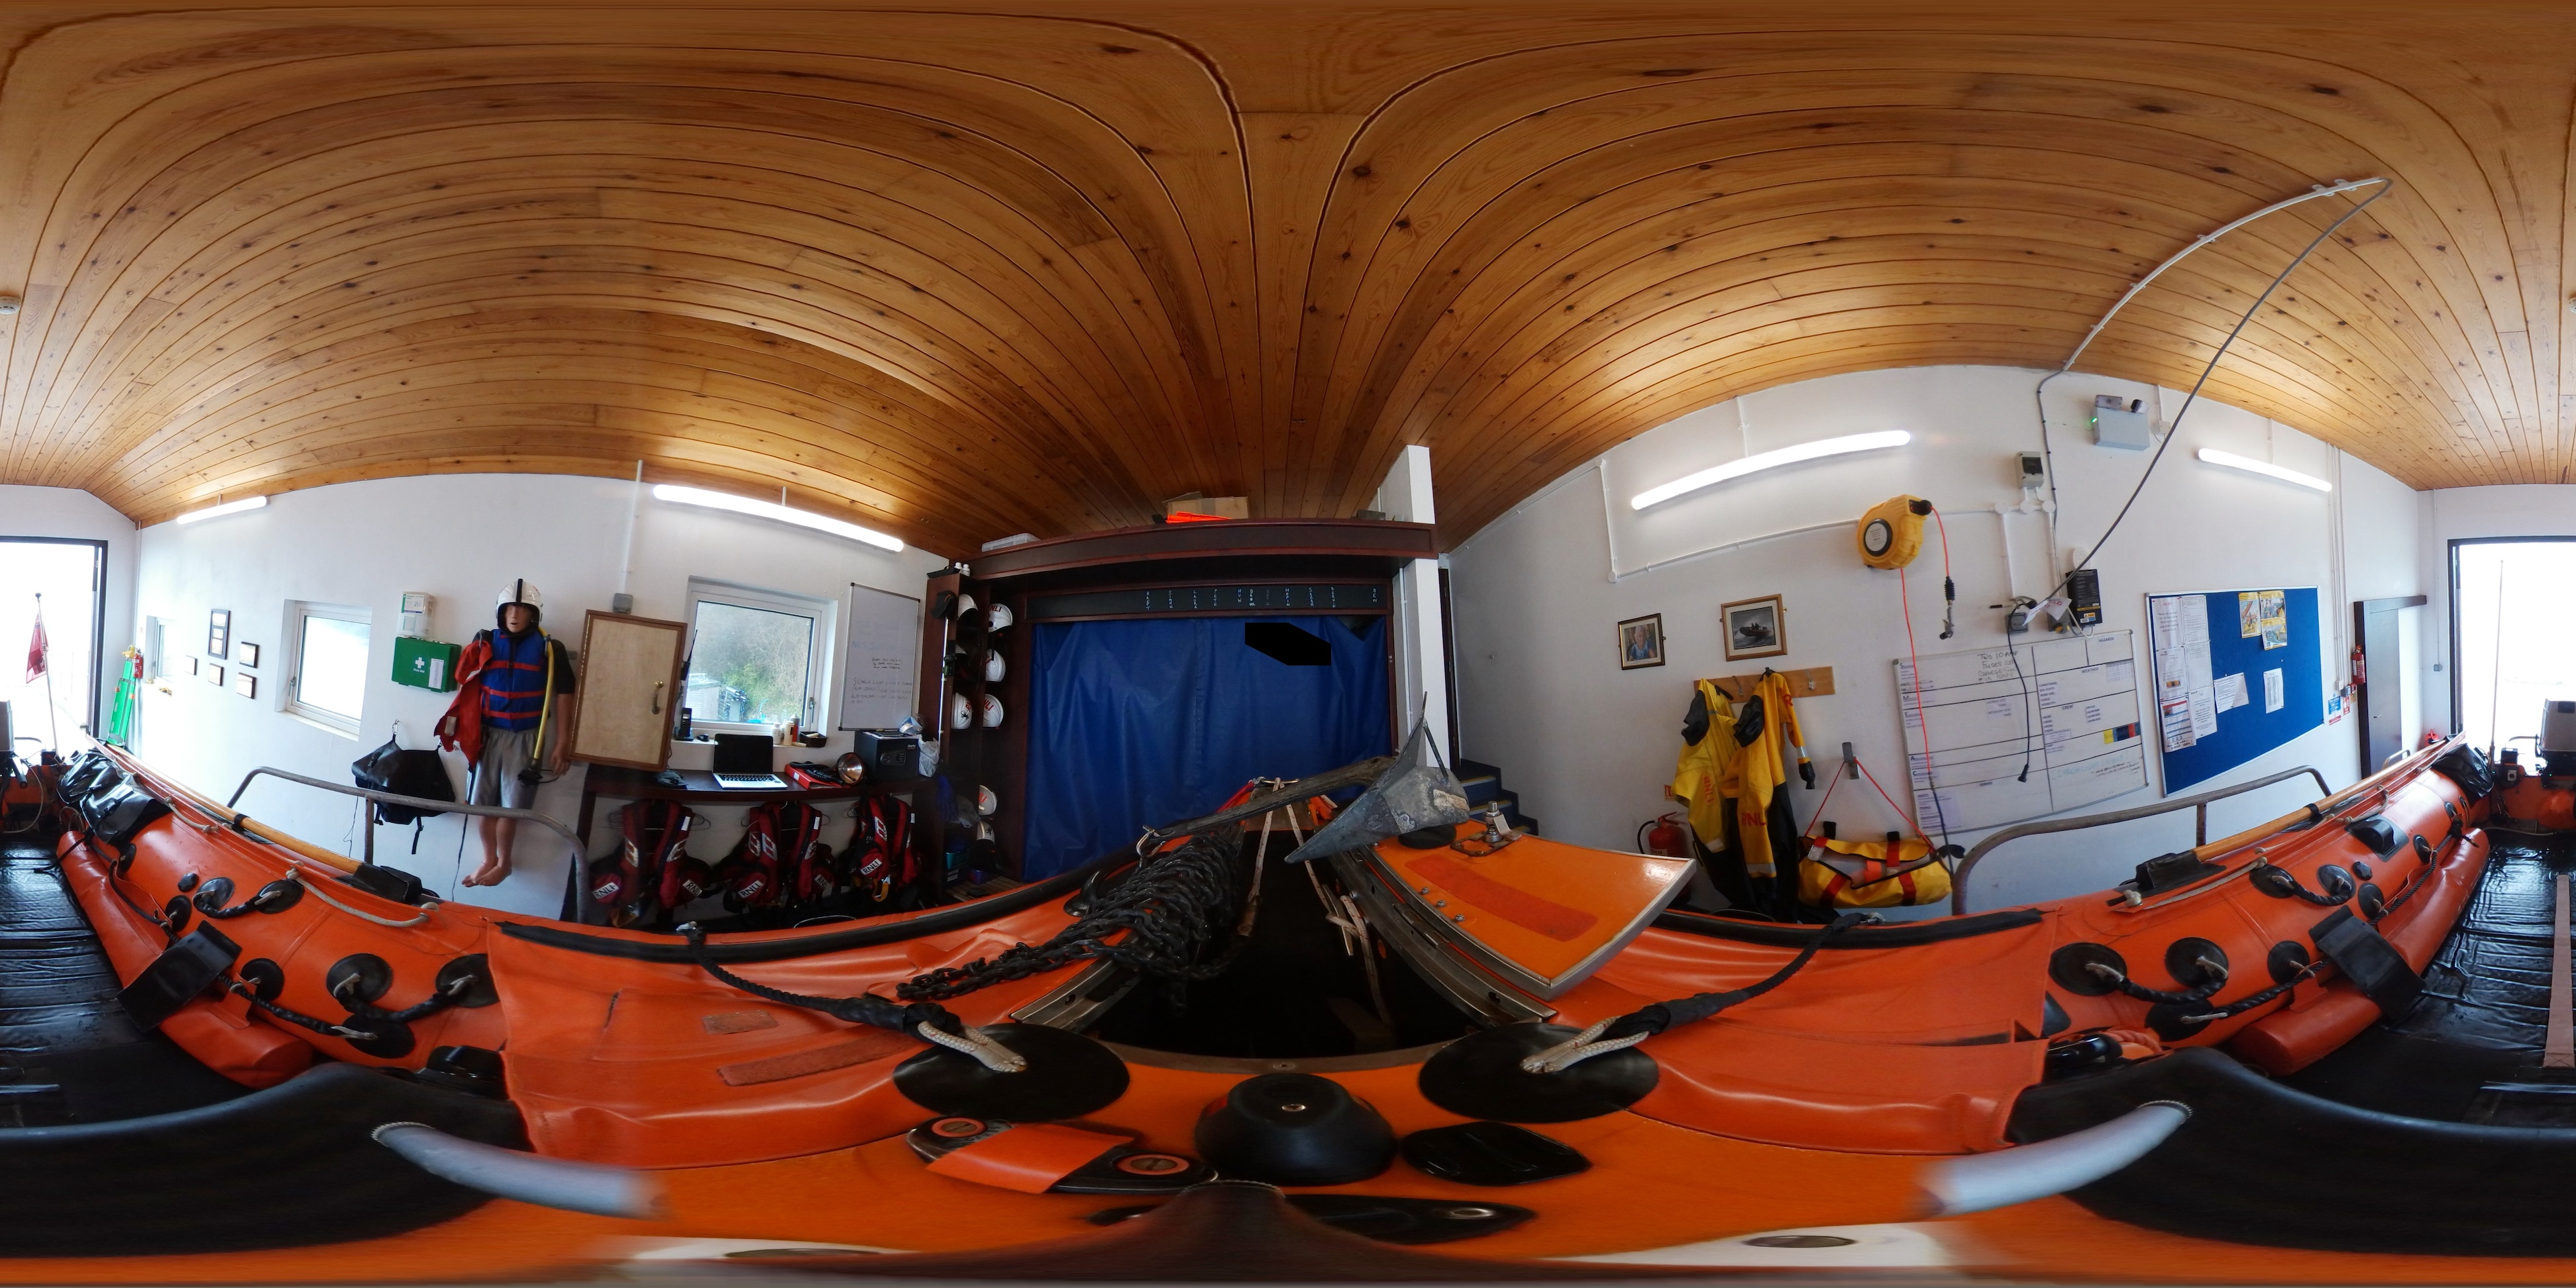
\includegraphics[width=1\textwidth]{images/360-items/anchor.JPG}
    \end{minipage}\hfill
    \begin{minipage}{0.3\textwidth}
        \centering
        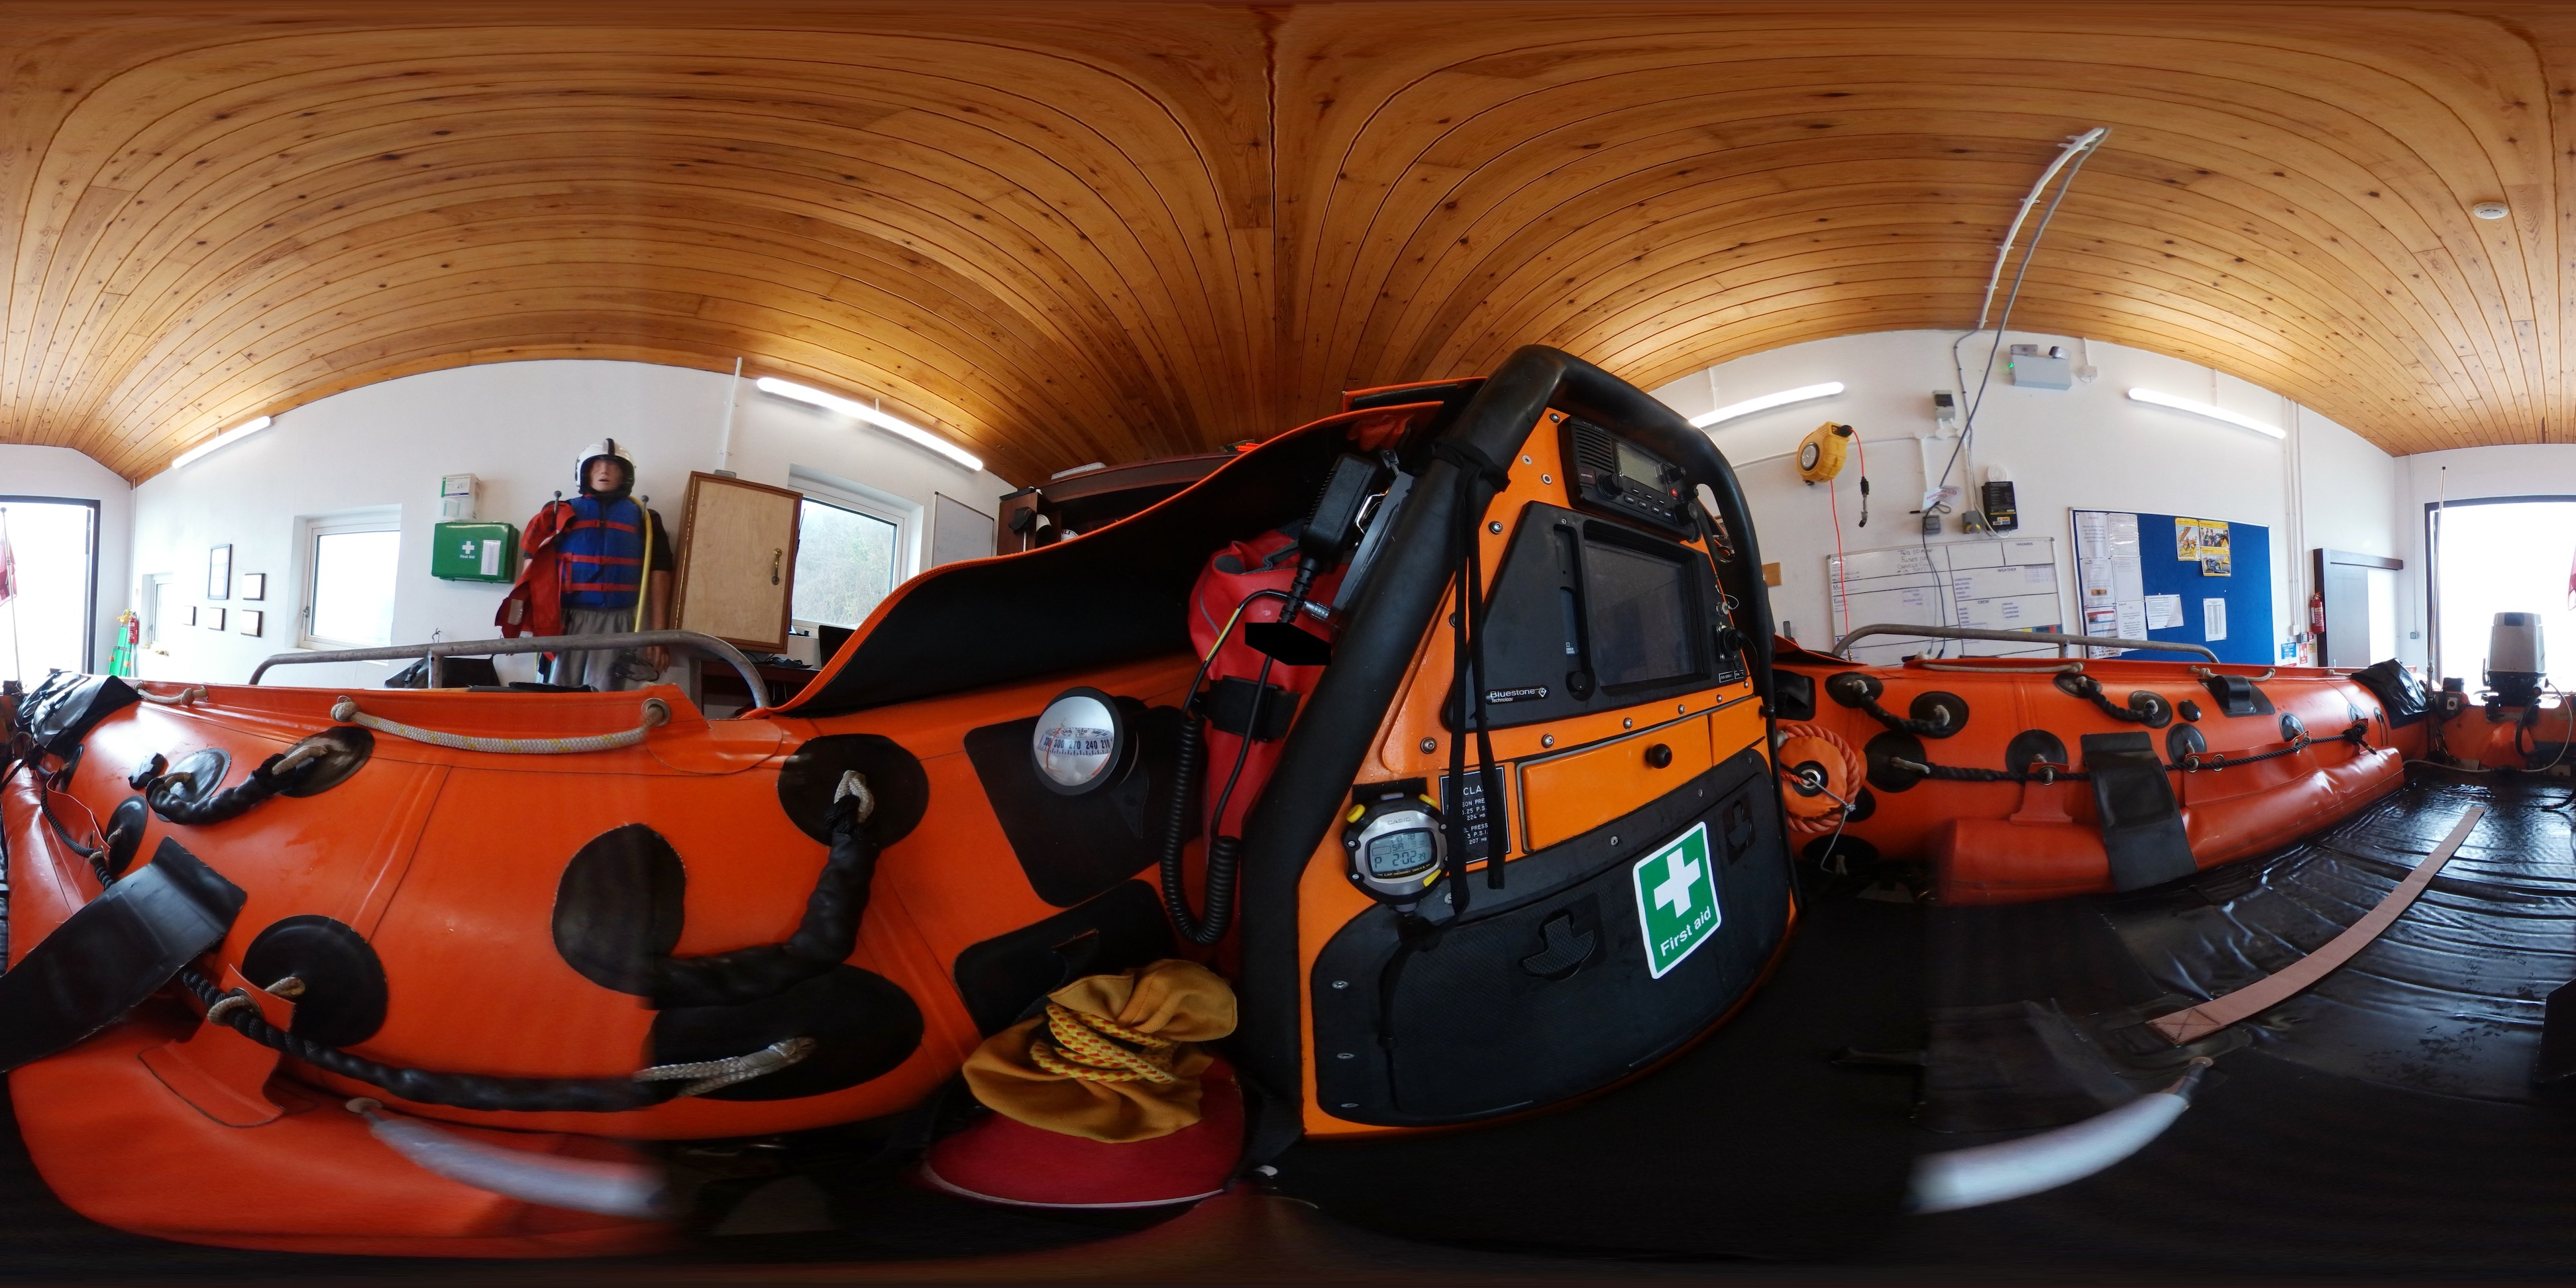
\includegraphics[width=1\textwidth]{images/360-items/compass.JPG}
    \end{minipage}\hfill
    \begin{minipage}{0.3\textwidth}
        \centering
        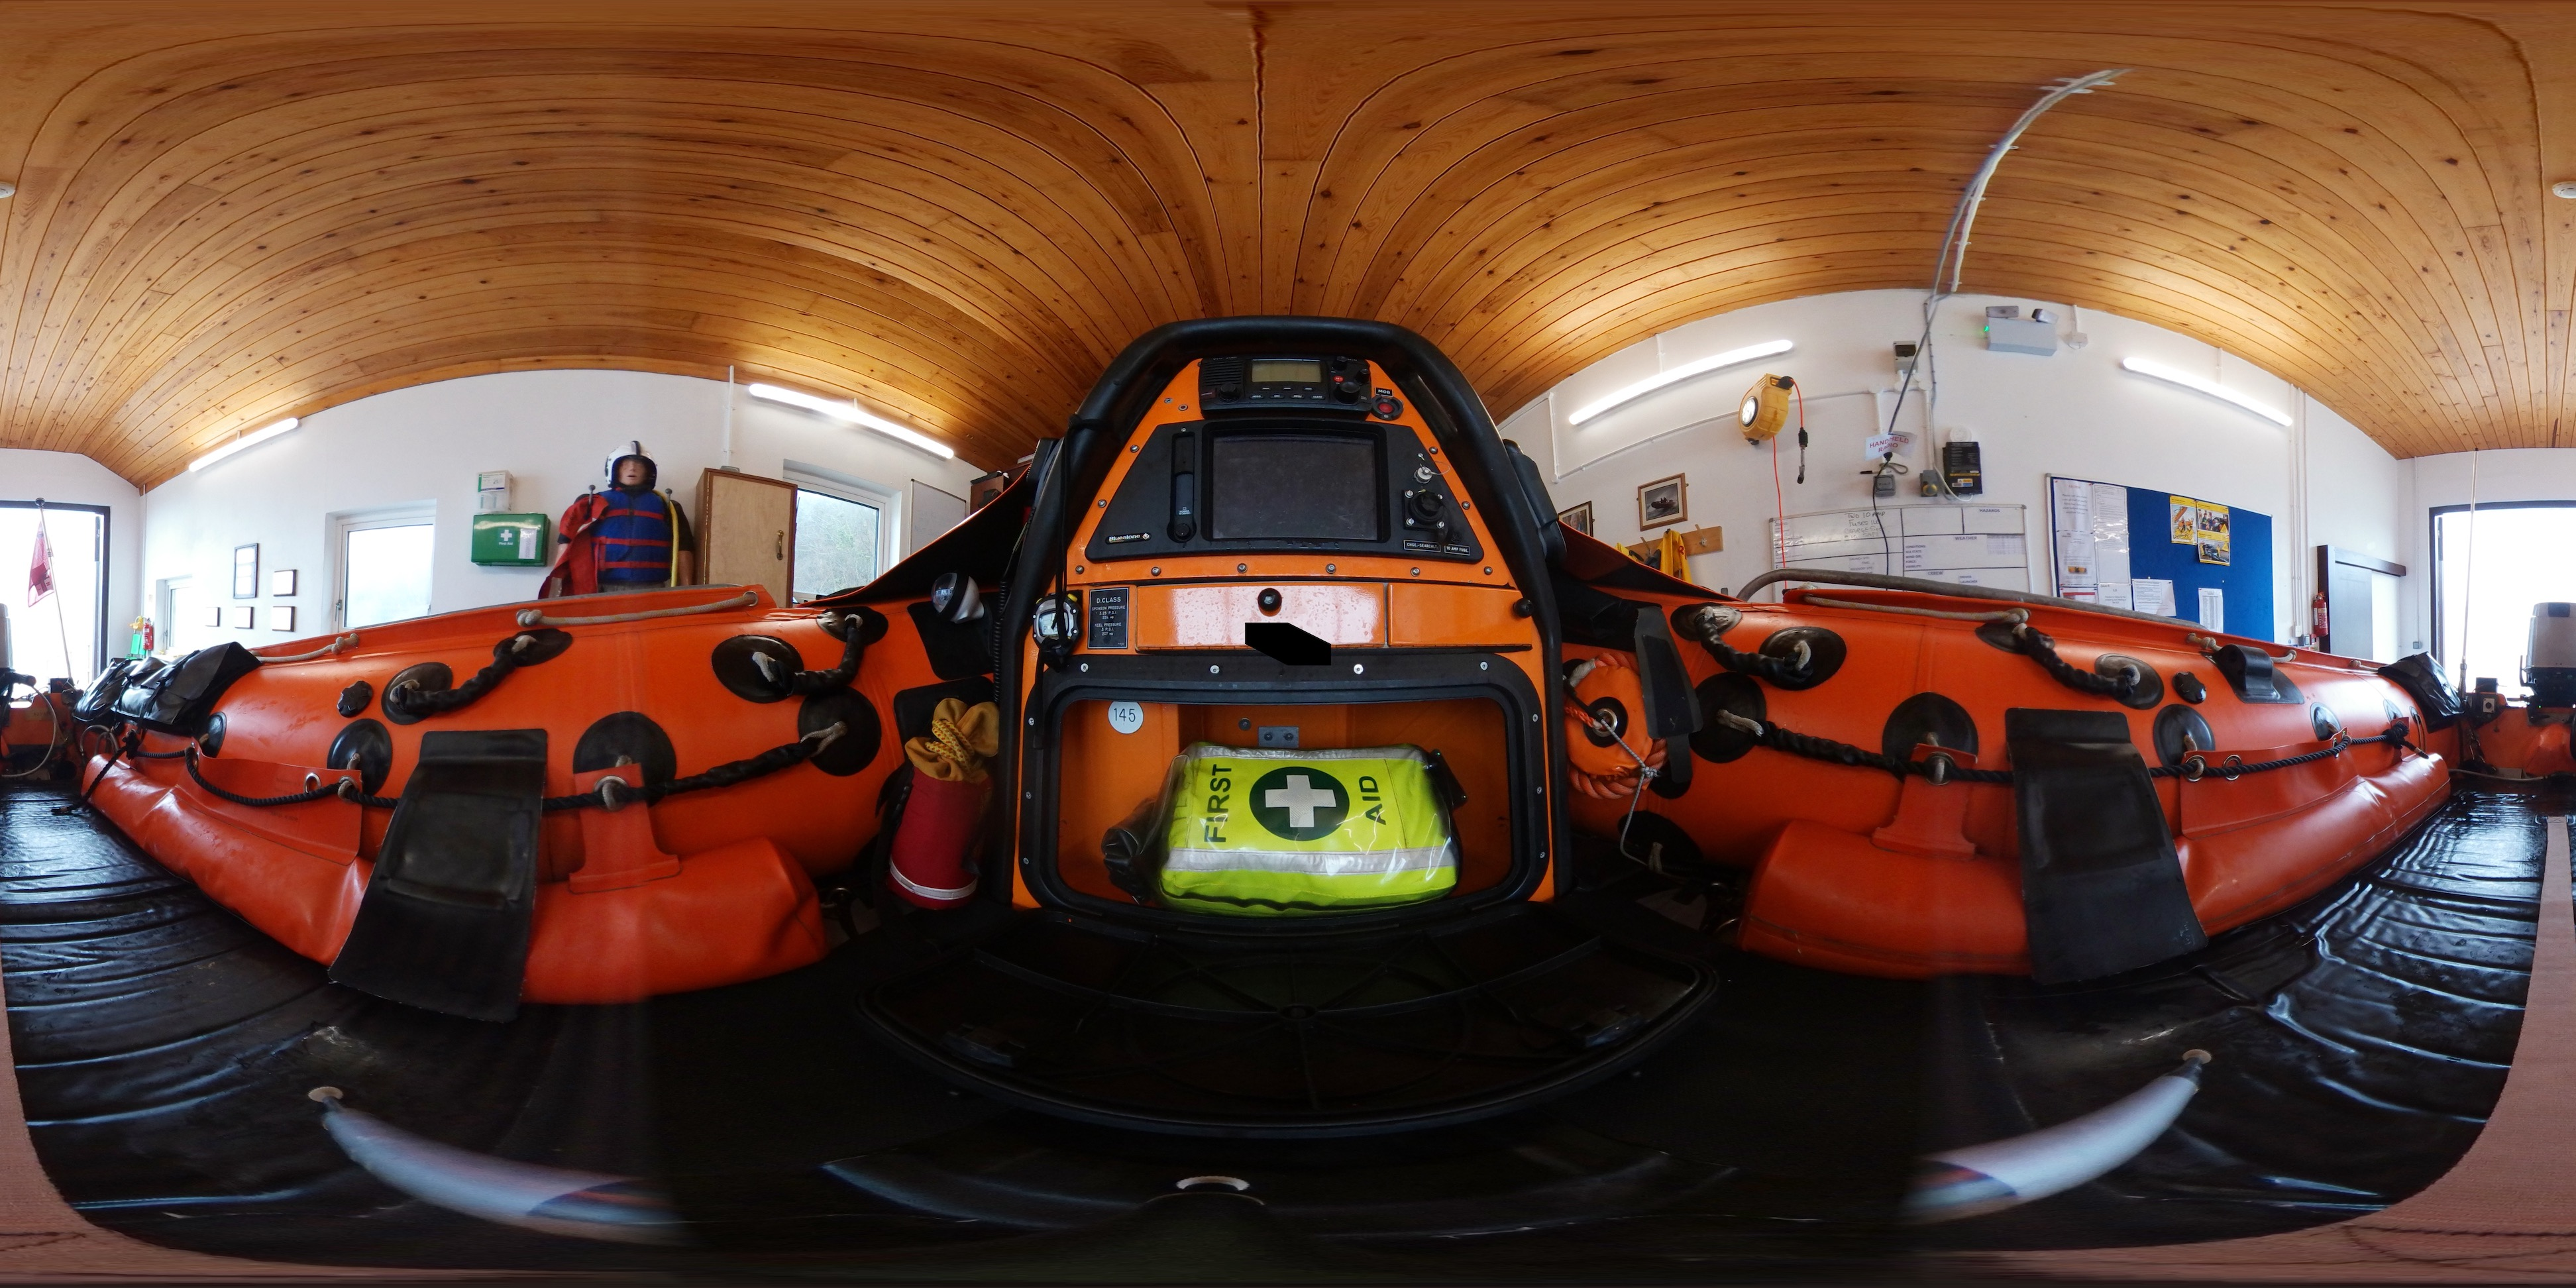
\includegraphics[width=1\textwidth]{images/360-items/firstaid.JPG}
    \end{minipage}\hfill
\end{center}
\begin{center}
    \centering
    \begin{minipage}{0.3\textwidth}
        \centering
        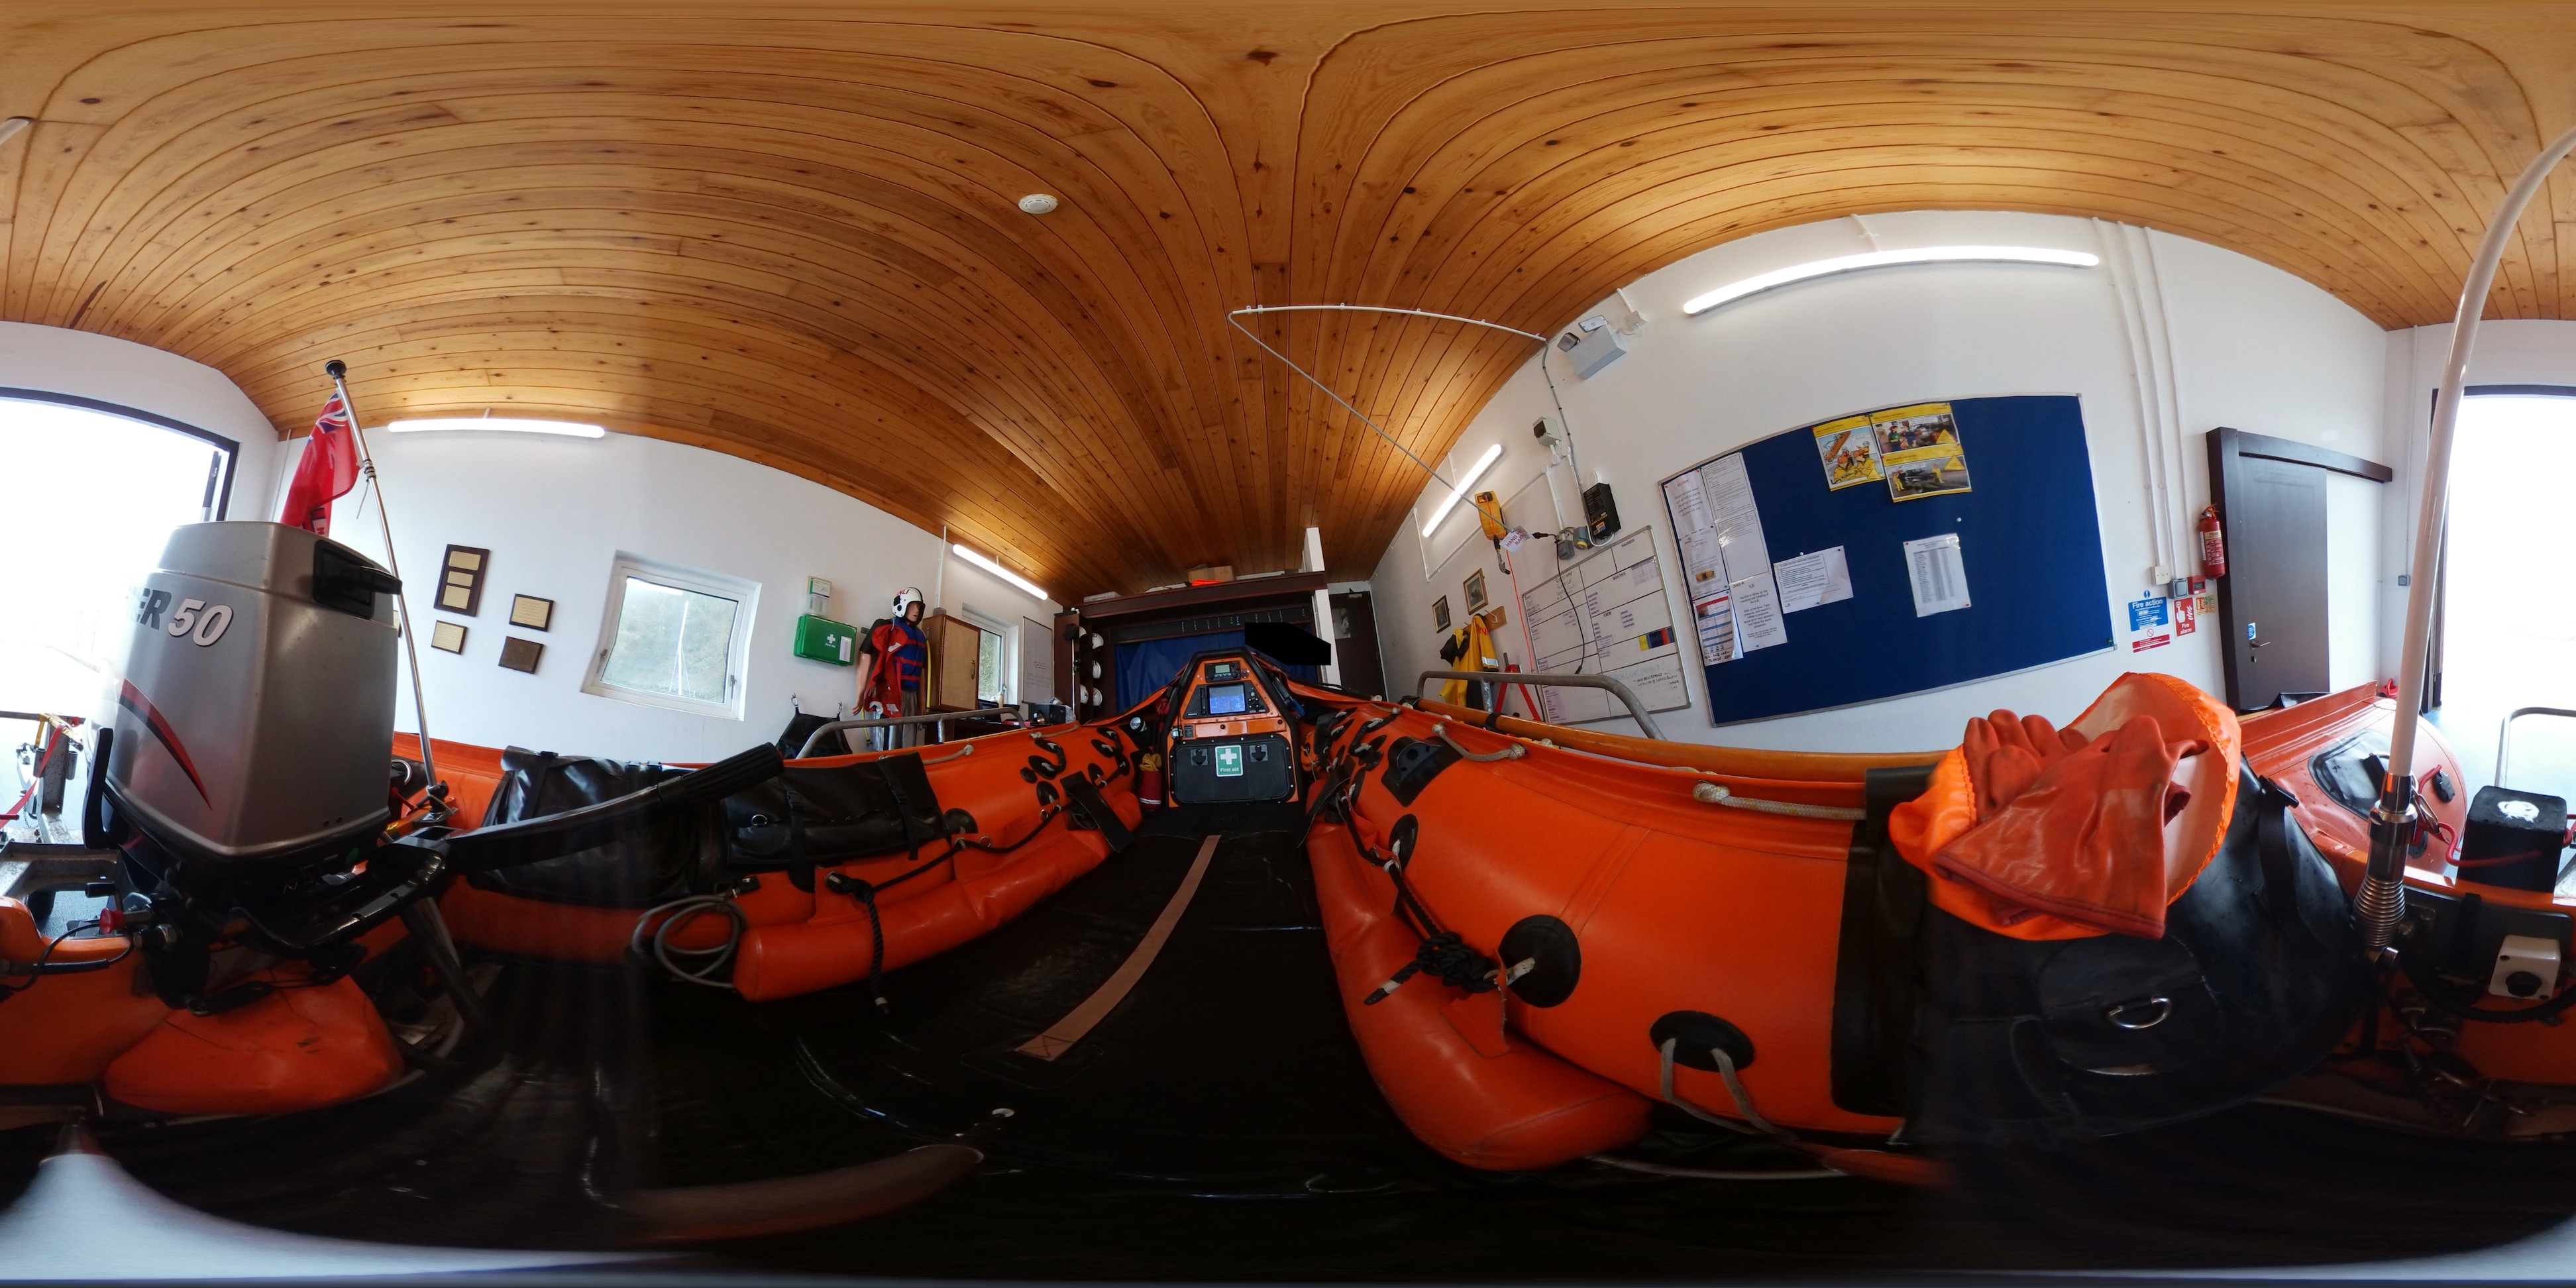
\includegraphics[width=1\textwidth]{images/360-items/gloves.JPG}
    \end{minipage}\hfill
    \begin{minipage}{0.3\textwidth}
        \centering
        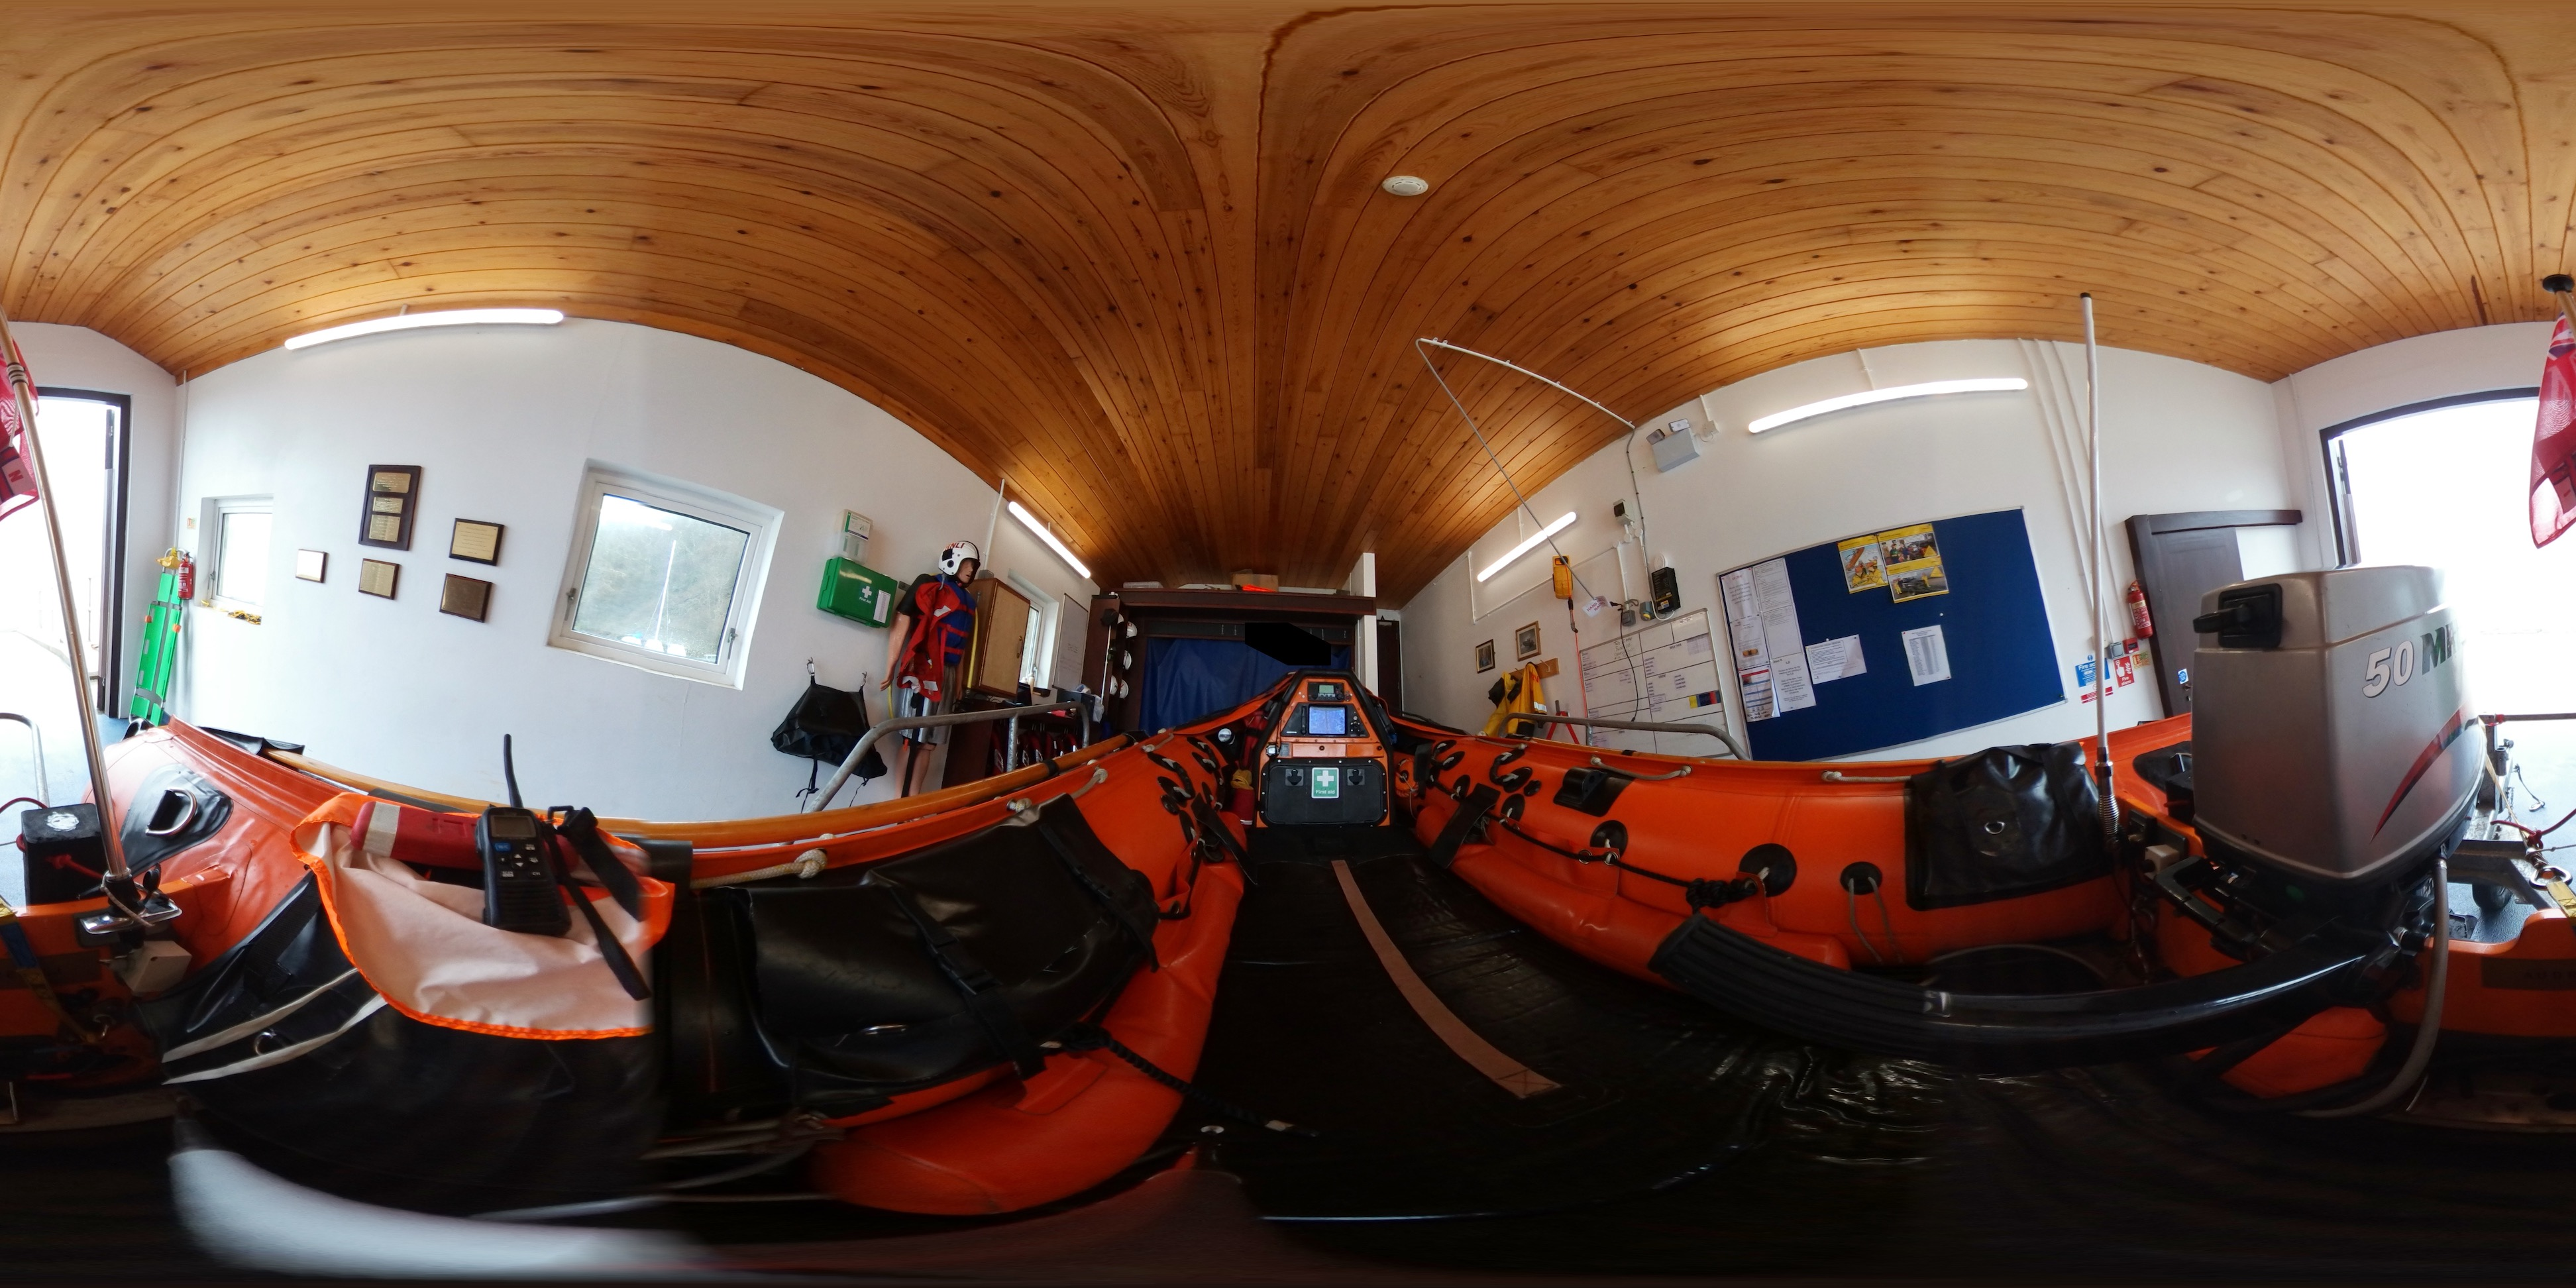
\includegraphics[width=1\textwidth]{images/360-items/handheld.JPG}
    \end{minipage}\hfill
    \begin{minipage}{0.3\textwidth}
        \centering
        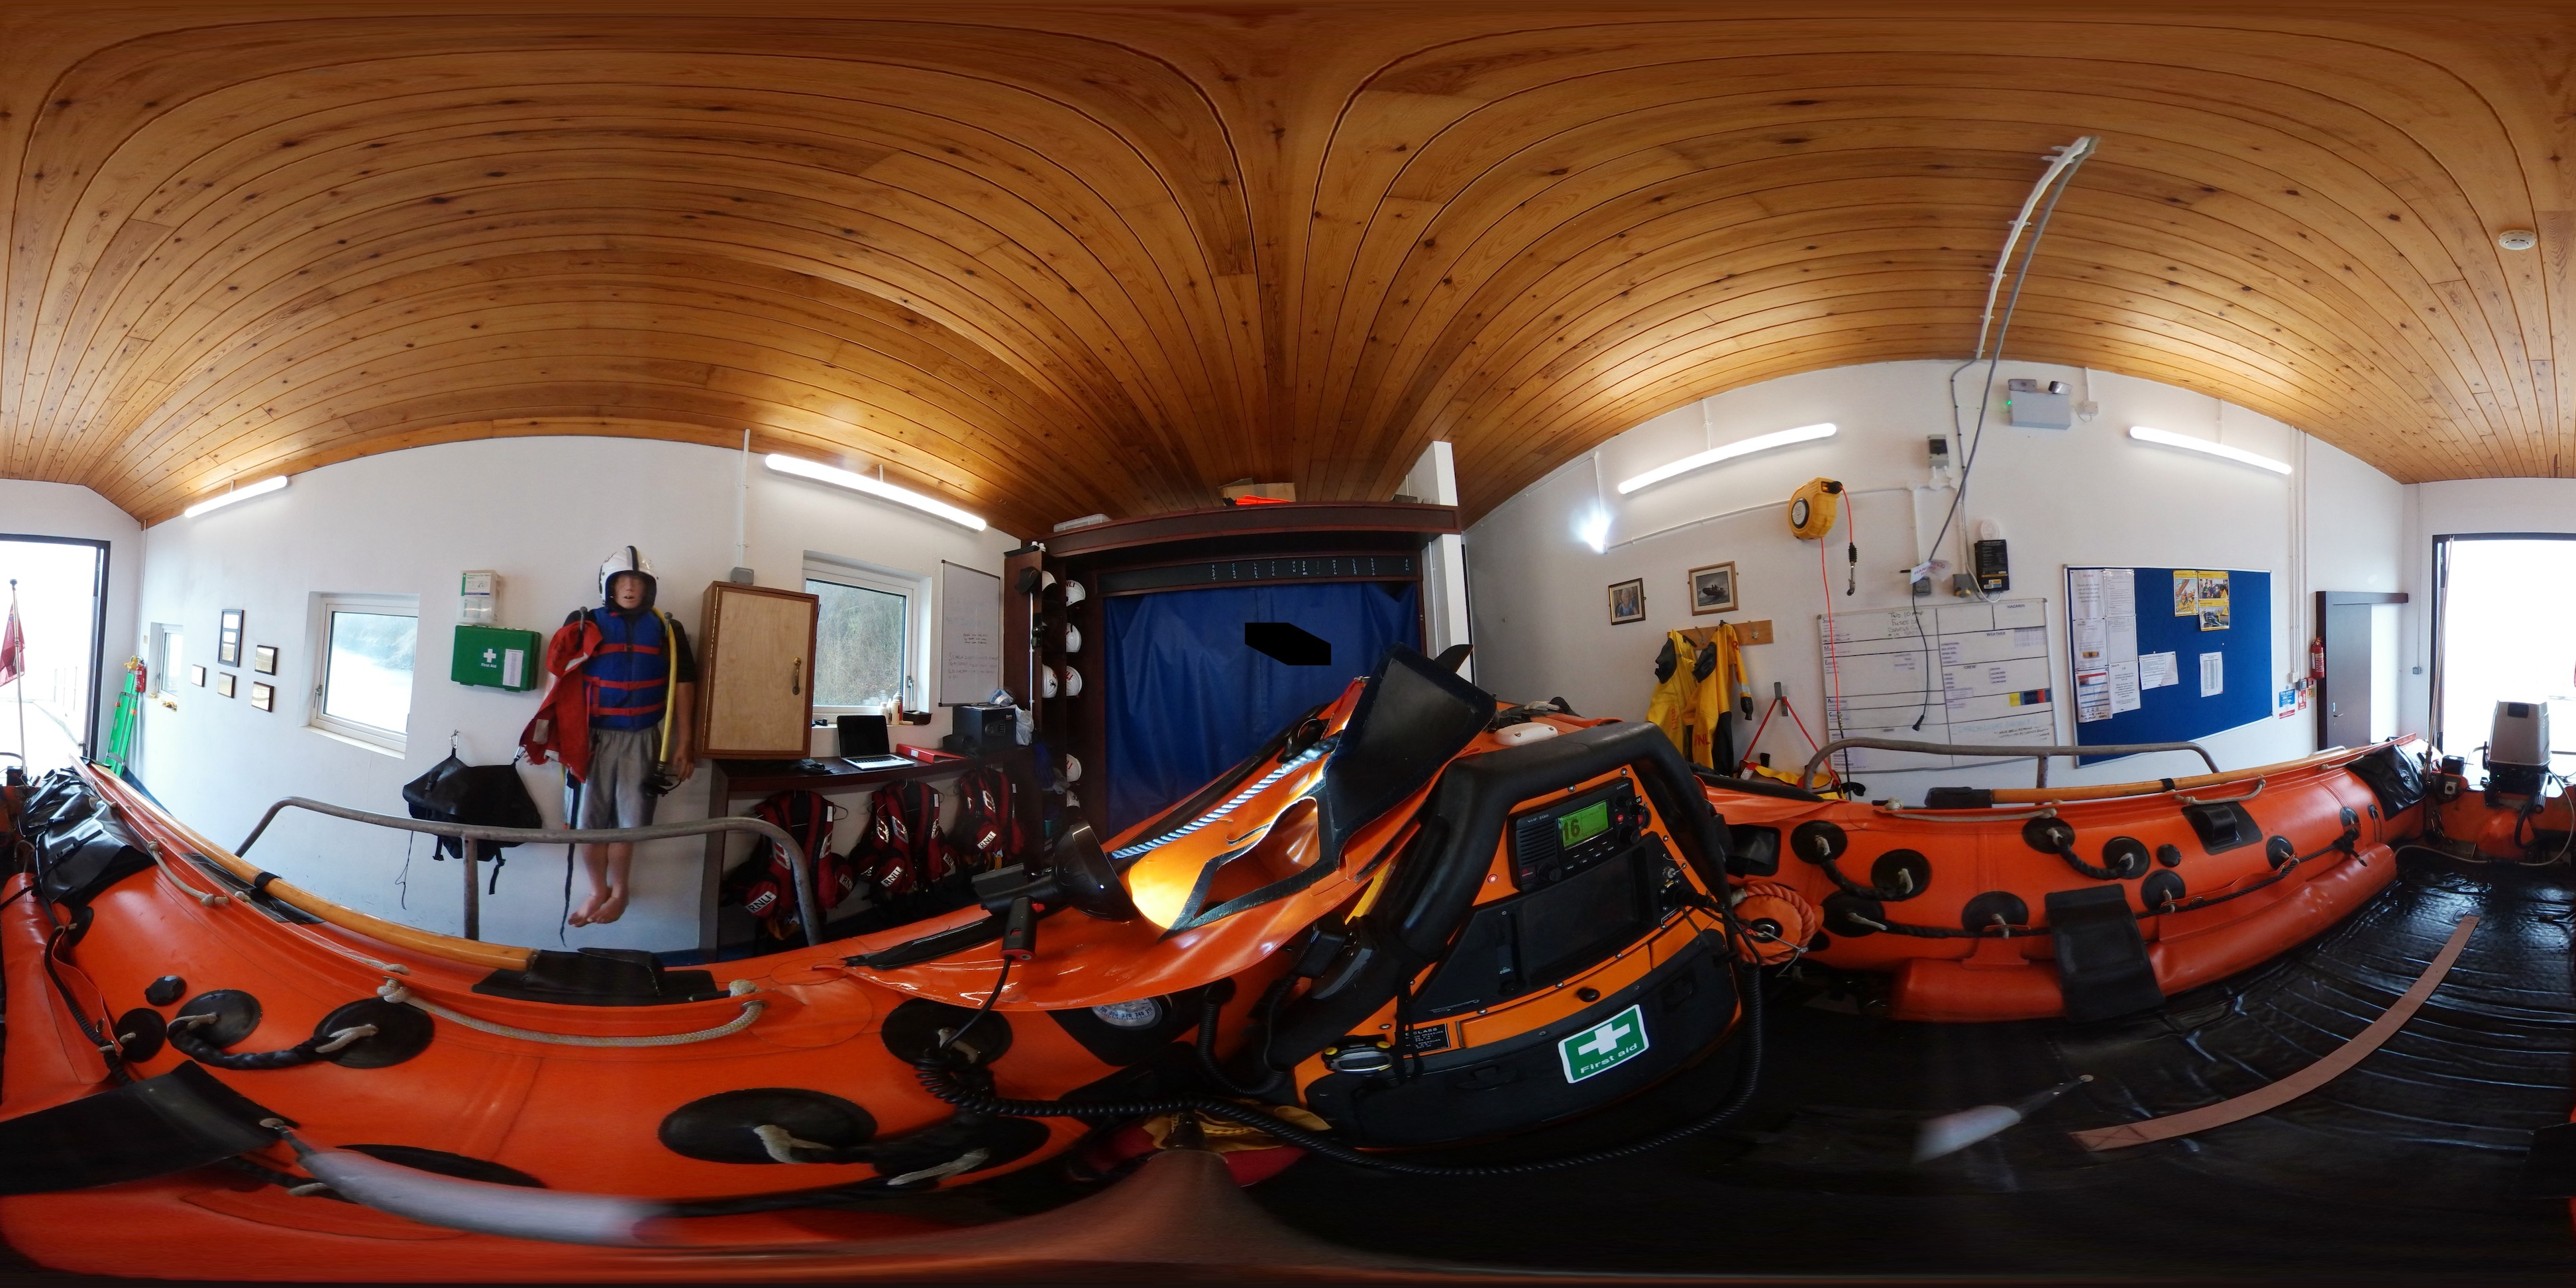
\includegraphics[width=1\textwidth]{images/360-items/light.JPG}
    \end{minipage}\hfill
\end{center}
\begin{center}
    \centering
    \begin{minipage}{0.3\textwidth}
        \centering
        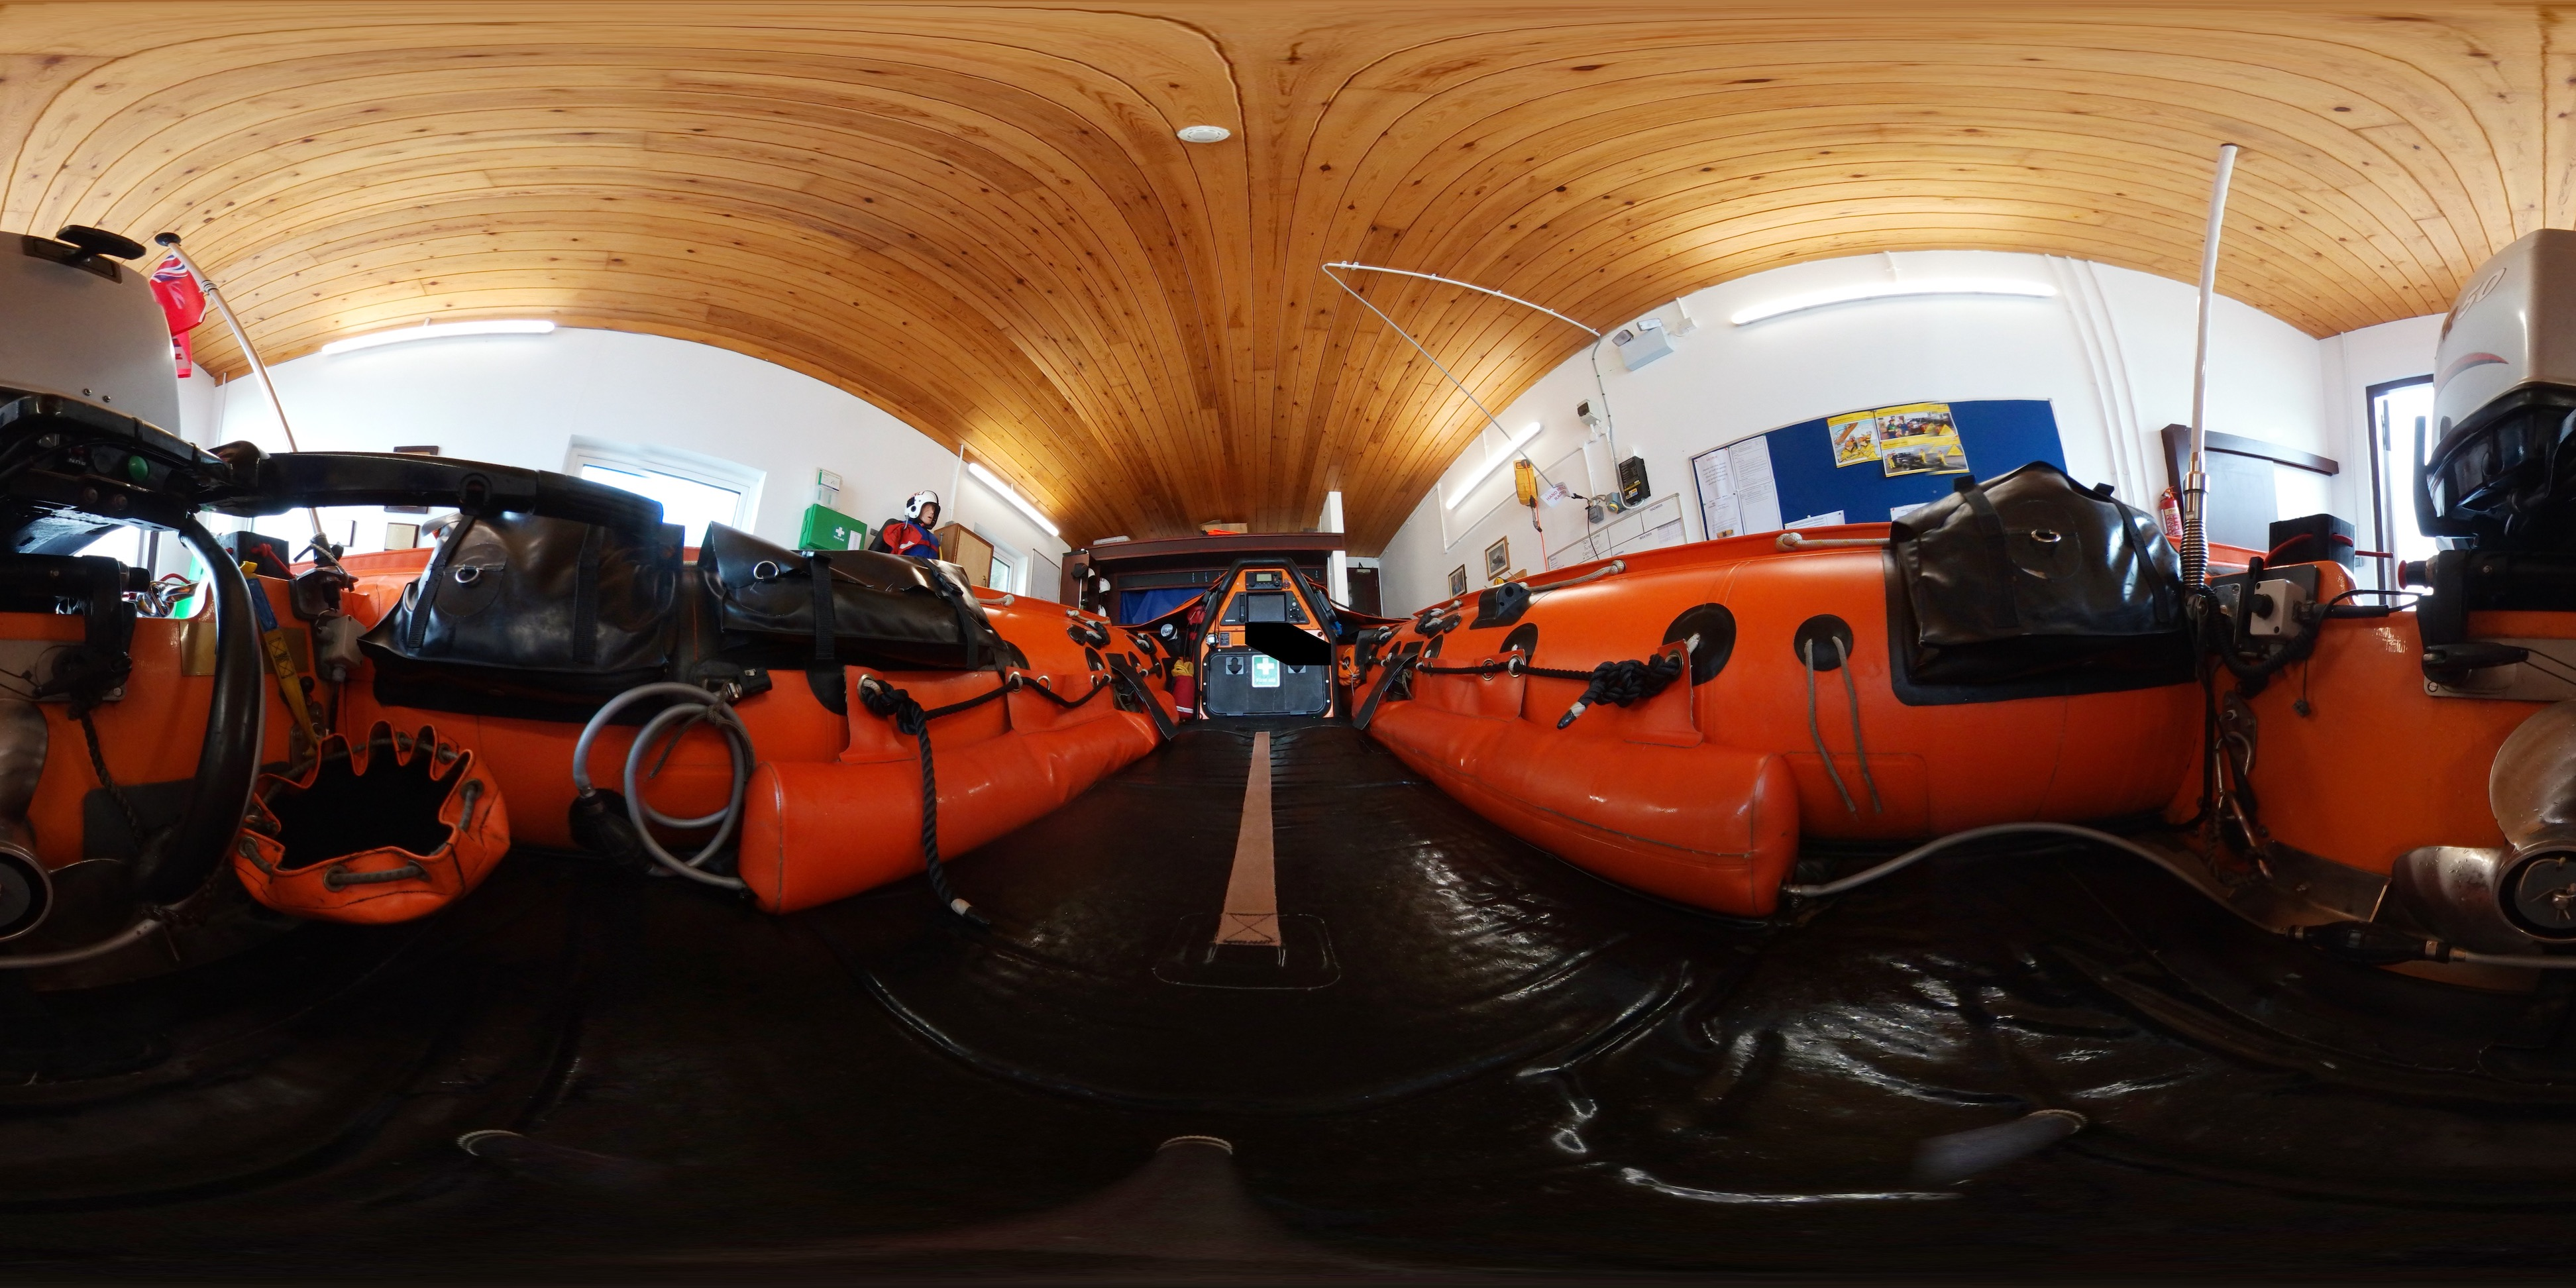
\includegraphics[width=1\textwidth]{images/360-items/propeller.JPG}
    \end{minipage}\hfill
    \begin{minipage}{0.3\textwidth}
        \centering
        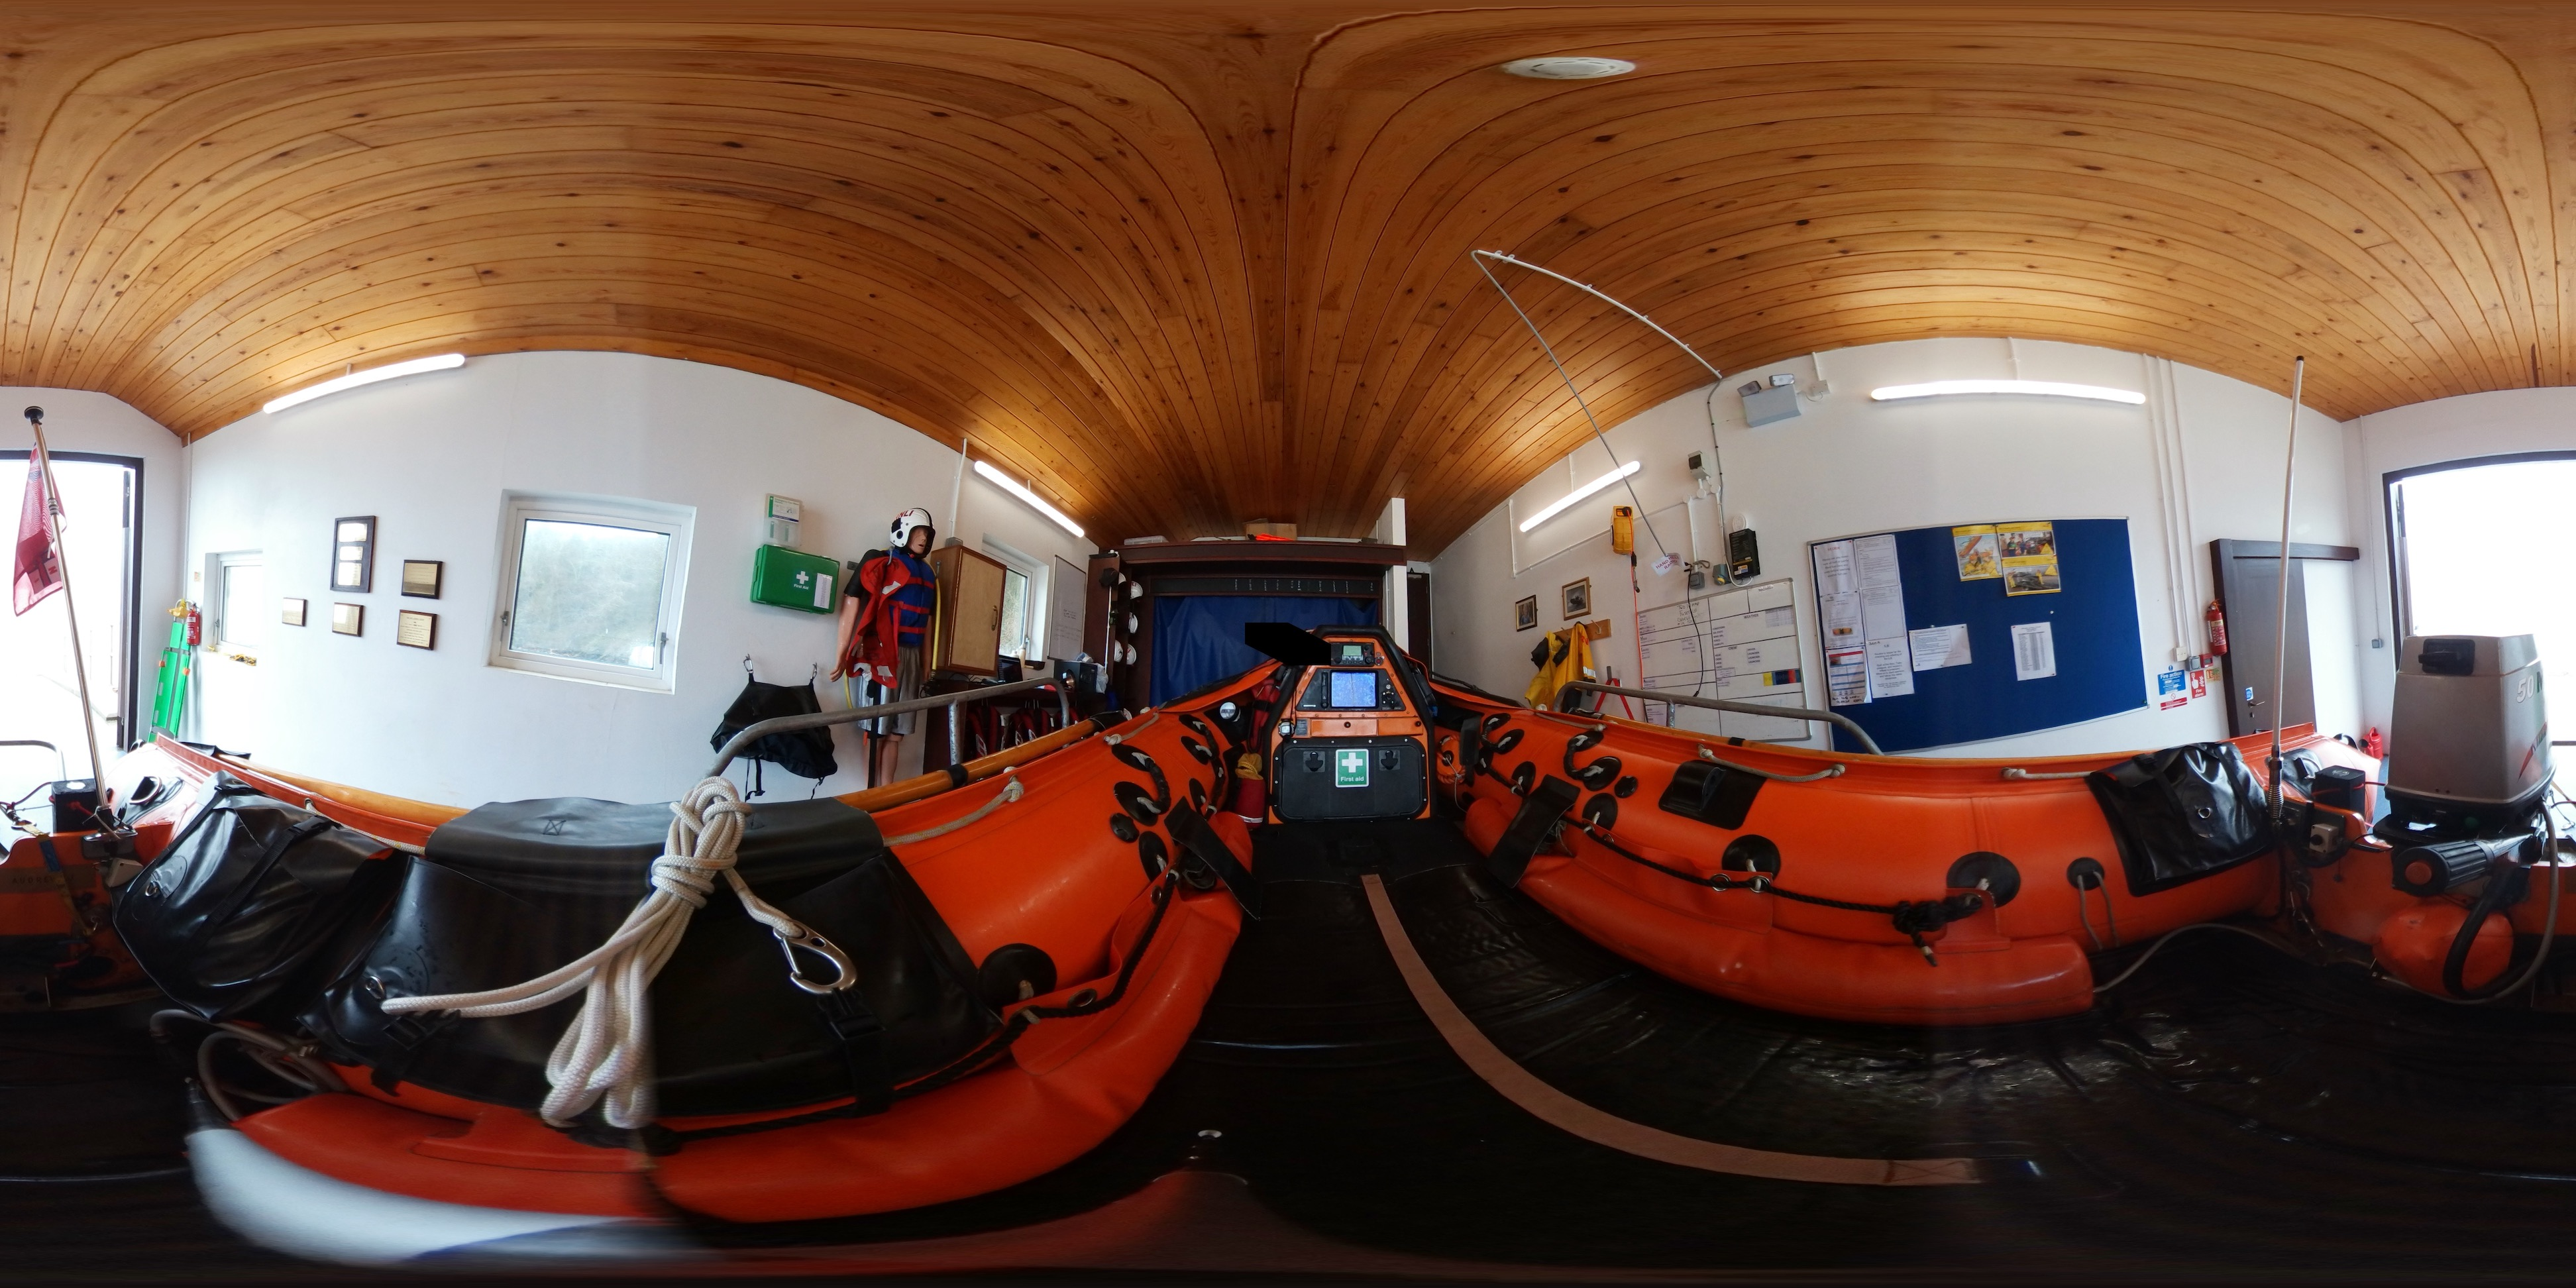
\includegraphics[width=1\textwidth]{images/360-items/towrope.JPG}
    \end{minipage}\hfill
    \begin{minipage}{0.3\textwidth}
        \centering
        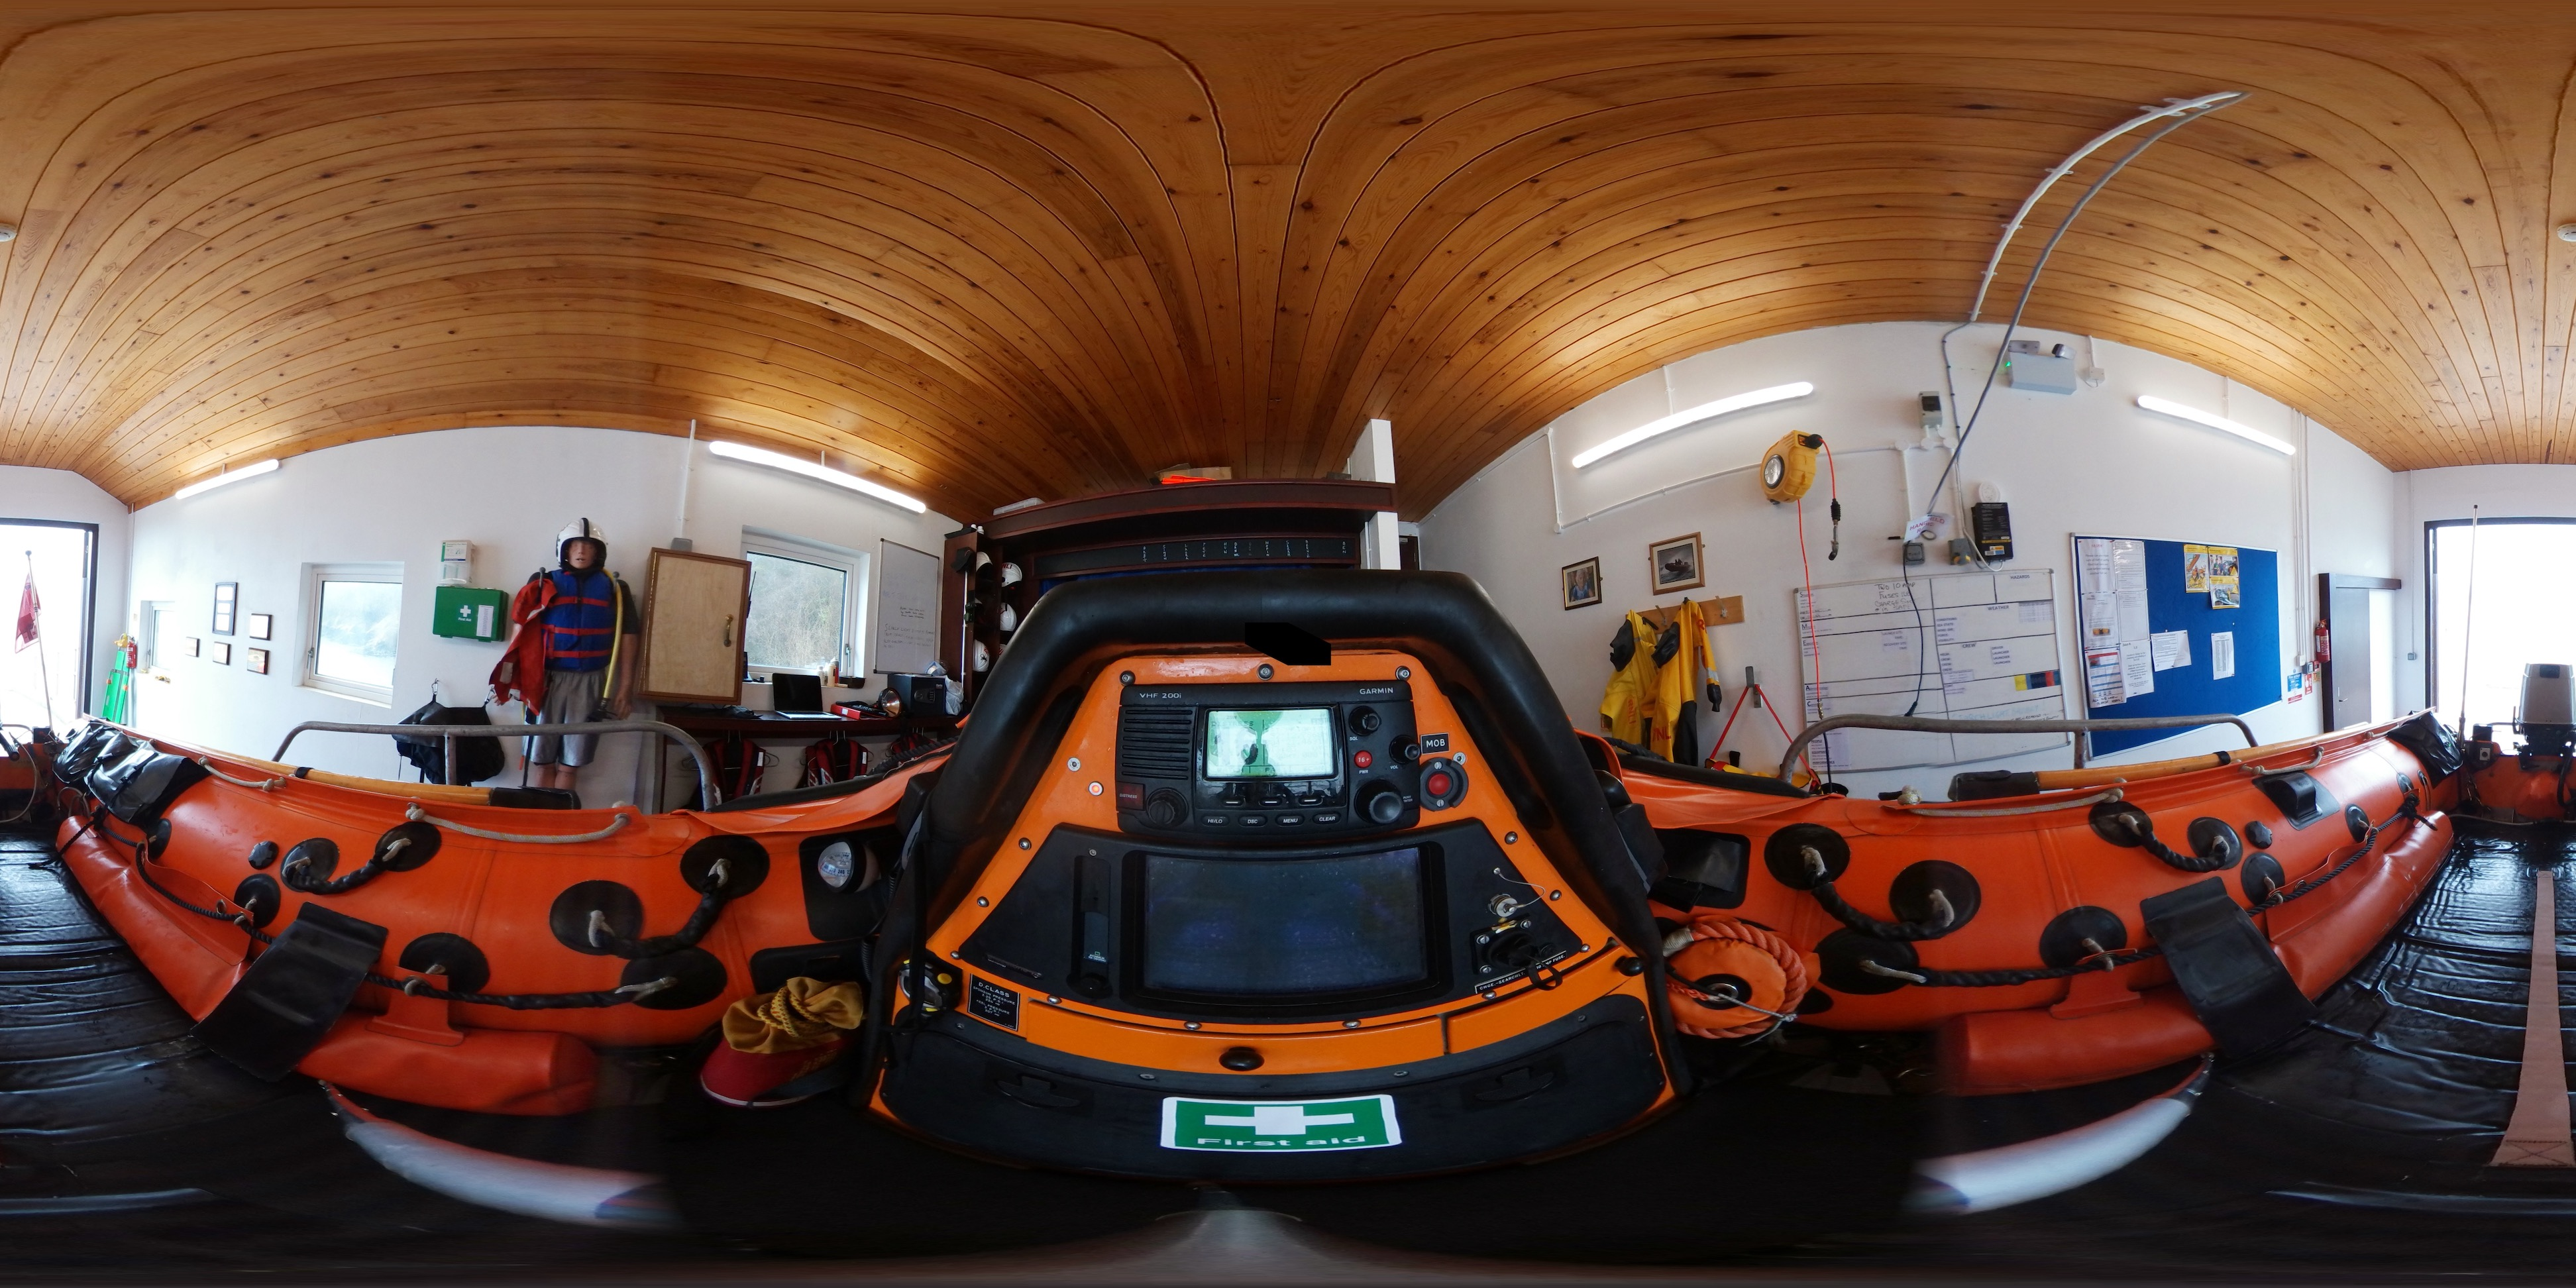
\includegraphics[width=1\textwidth]{images/360-items/vhf.JPG}
    \end{minipage}\hfill
\end{center}
\captionof{figure}{360-degree images taken with the Samsung Gear 360 of the nine items which each user will recall.}
\label{360-items}
\end{minipage}

\begin{center}
    \centering
    \begin{minipage}{0.4\textwidth}
        \centering
        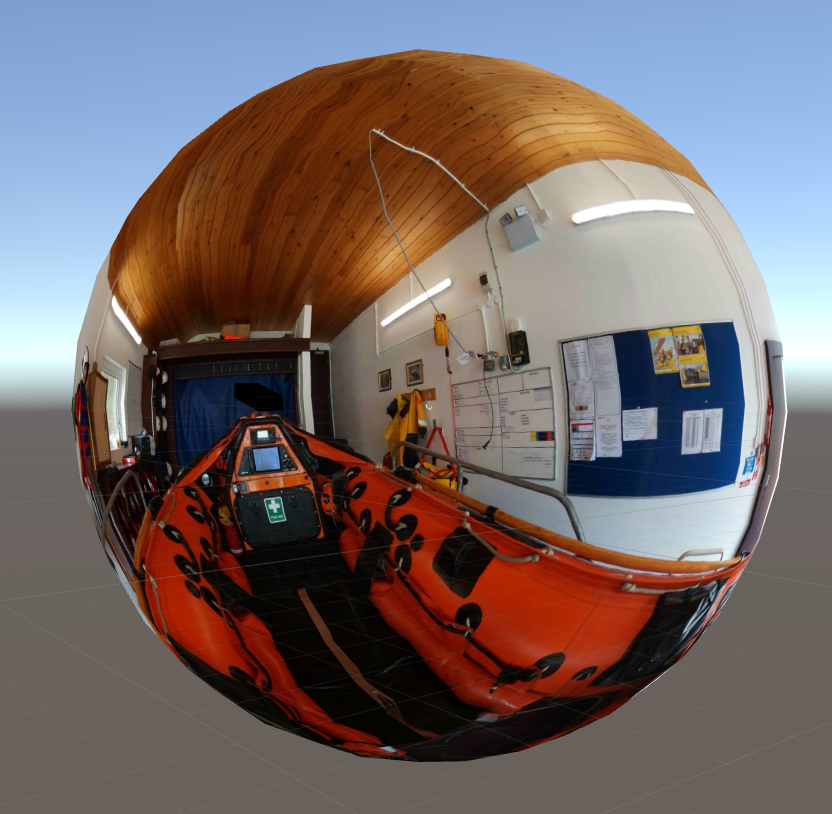
\includegraphics[width=1\textwidth]{images/360-sphere.png}
        \captionof{figure}{Screenshot of the material on the sphere object}
        \label{360-sphere}
    \end{minipage}\hfill
    \begin{minipage}{0.4\textwidth}
        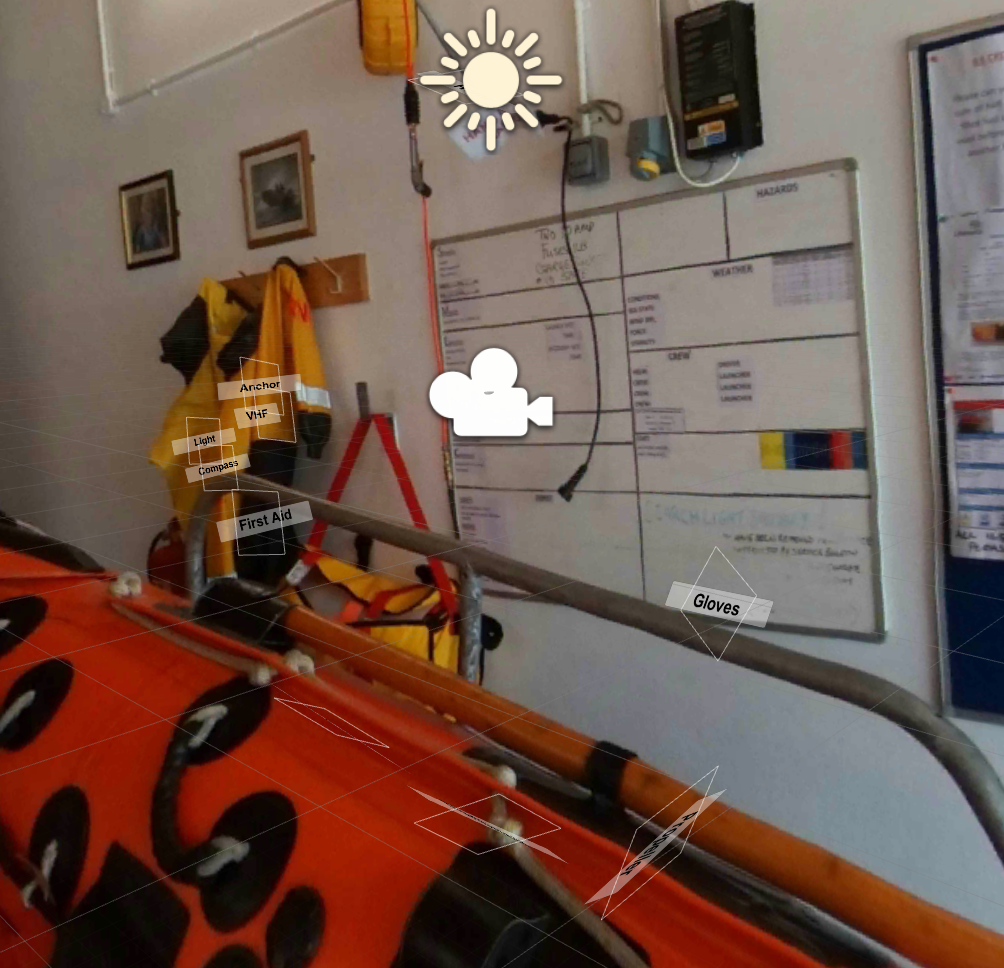
\includegraphics[width=1\textwidth]{images/360-overview.png}
        \captionof{figure}{Screenshot demonstrating the layout of the 360 environment, with camera object, UI labels, and 360-image background}
        \label{360-overview}
    \end{minipage}\hfill
\end{center}

\subsection{Unity}
Unity makes constructing 360-degree environments trivial. As detailed in a Unity blog post in 2017 \footnote{How to integrate 360 video or images with Unity \url{https://blogs.unity3d.com/2017/07/27/how-to-integrate-360-video-with-unity/}}: 

\begin{itemize}
\item Add Image to shader of material
\item Add material to sphere in the scene, Figure \ref{360-sphere}
\item Place camera within sphere, Figure \ref{360-overview}
\end{itemize}

Using the steps above it becomes simple to construct an environment within Unity which places a user within a 360-environment. Now, in order to allow a user to explore an environment there simply needs to be a material for each 360-image, which is changed to according to user input. For example, if a user would like to see inside a container, the user can click that container, then the material of the sphere changes to an image with a close up view of the open container. This creates the illusion that a user is moving around a scene, and is detailed in Section \ref{interaction}. 

\section{Google VR, Scene Interaction, and Deployment}
During the development phase and early testing, it was concluded that it was disorienting to have transformation within the 360-video scene, and thus it was concluded that the 360-image environment would use static images. In order to maintain consistency it was concluded that the CG environmnet would need to also have a statically positioned camera; although both environments would obviously allow rotational camera movement.  

\subsection{Google VR}\label{googlevr}

In order to implement a camera which could be controlled using the Google Daydream View headset, Google offers a free unity package for Google VR projects \footnote{Releases \url{https://github.com/googlevr/gvr-unity-sdk/releases}}. This is imported into Unity. The package has an abundance of resources such as demo scenes, and prefabs. From this package the required prefabs are \lstinline{GvrHeadset, GvrControllerMain, GvrControllerPointer}. Finally, the \lstinline{GvrPointPhysicsRaycaster} script must be applied to the main camera. These steps allow a users to control the rotation of the camera with the headset, and use the controller to control the reticle within the scene. 

\subsection{Interaction}\label{interaction}

\subsubsection{UI}
The elements which a user interacts with in the 360-image environment are UI labels. Following the steps outlined in Section \ref{googlevr}, a panel object within the scene with its Raycast Target option set to true is all that is necessary for the UI element to be interactive. These elements are then placed overlaying each of the nine objects; for the CG environment this can be seen in Figure \ref{model}, and in Figure \ref{360-labels}. 

\begin{minipage}{\textwidth}
    \centering
    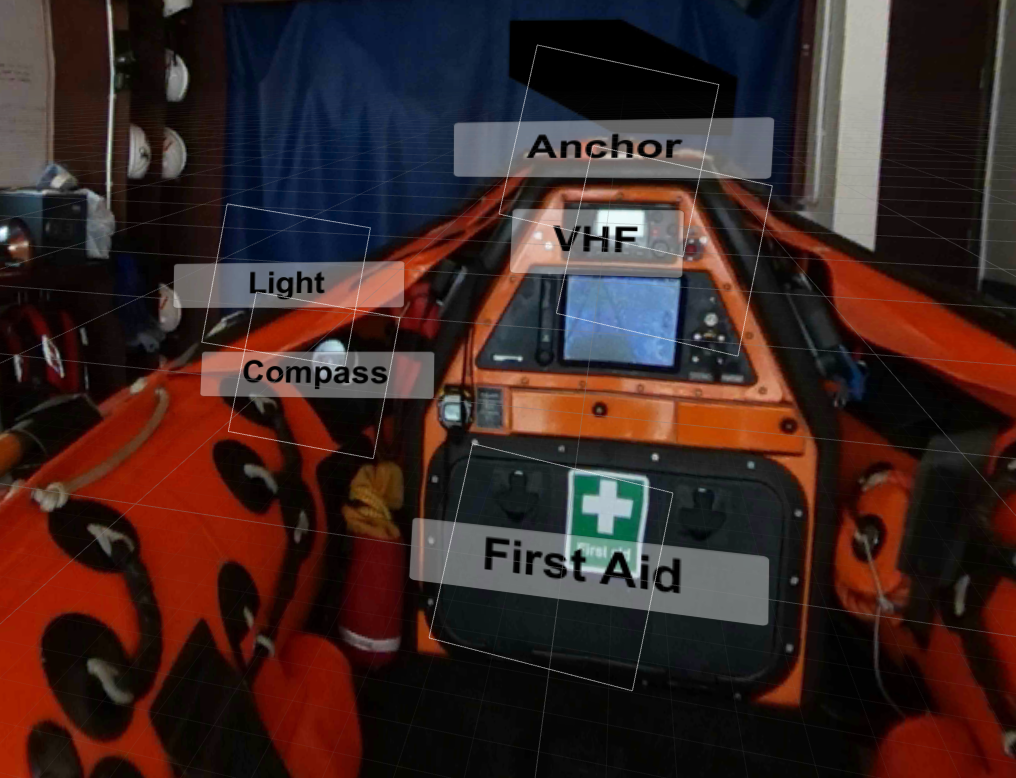
\includegraphics[width=0.6\textwidth]{images/360-labels.png}
    \captionof{figure}{Screenshot of UI Labels overlaid onto 360-image in Unity.}
    \label{360-labels}
\end{minipage}
    

\begin{minipage}{\textwidth}
    \centering
    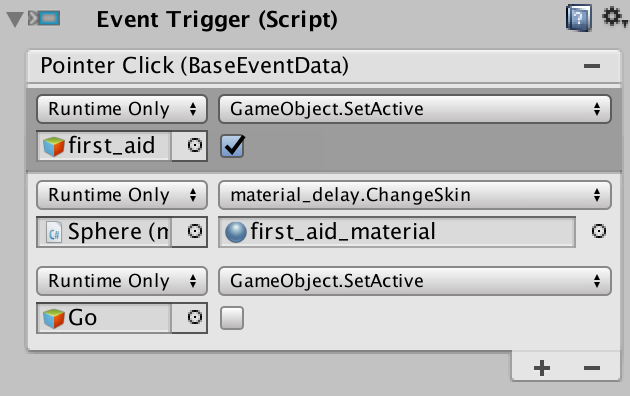
\includegraphics[width=0.35\textwidth]{images/360-event-component.png}
    \captionof{figure}{Screenshot of the Event Trigger component attached to each UI label in the 360-environment.}
    \label{360-event}
\end{minipage}


In the 360-image environment it is these labels that have event trigger components, illustrated in Figure \ref{360-event}. After a user selects a UI label, the material of the sphere changes to the image which showcases that specific element.

In the computer-generated environment it is the objects themselves, or the hatches to those objects which a user interacts with. Each of the interactable objects have colliders, and event trigger components. An additional feature of the CG environment is that the hatches are animated; the event trigger component for these objects is shown in Figure \ref{cg-event}. This event trigger calls the \lstinline{GoToLocation} function, shown in Figure \ref{location}. 

\begin{minipage}{\textwidth}
\centering
\begin{lstlisting}
	public GameObject player;

	public void GoToLocation(GameObject location) {
		player.transform.position = location.transform.position;
	}
\end{lstlisting}
\captionof{figure}{Code snippet for changing player location.}
\label{location}
\end{minipage}

\begin{minipage}{\textwidth}
    \centering
    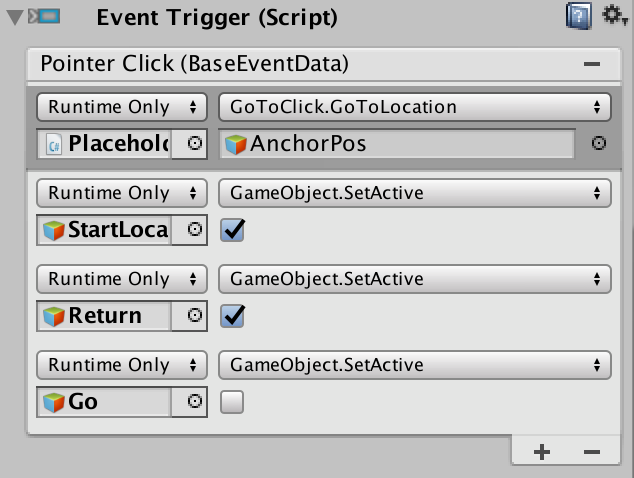
\includegraphics[width=0.35\textwidth]{images/CG-event-component.png}
    \captionof{figure}{Screenshot of the Event Trigger component attached to each interactable object in the CG-environment.}
    \label{cg-event}
\end{minipage}


To animate the hatches, or objects themselves, each animated object has an animator component with a controller as shown in Figure \ref{animator}. The animator controller operates as a state diagram, this can be useful to ensure the order of animations are correct - i.e. an open container should not play an animation of it opening. An important note to make is that each animation in the controller should have its \lstinline{Loop Time} checkbox unselected; each transition should also have their \lstinline{Exit Time} checkbox set to false. 

To animate these objects when a user clicks the controller, the \lstinline{PerformRaycast} function in the \lstinline{GvrPointerPhysicsRaycaster} script is appended to contain the code snippet in Figure \ref{anim_script}. All animated objects have a tag of \lstinline{"Bag"} and a state of either 1 or 0 which indicates if that object is open or closed. 

\begin{minipage}{\textwidth}
\begin{lstlisting}
if (item.tag == "Bag" && item.GetComponent<State> ().state == 0) {
	if (trigger) {
		anim = item.GetComponent<Animator> ();
		anim.Play ("open_bag");
		item.GetComponent<State> ().state = 1;
	}
}	
else if (item.tag == "Bag" && item.GetComponent<State> ().state == 1) {
	if (trigger) {
		anim = item.GetComponent<Animator> ();
		anim.Play ("close_bag");
		item.GetComponent<State> ().state = 0;
	} 
}

\end{lstlisting}
\captionof{figure}{Code snippet for playing animation of object.}
\label{anim_script}
\end{minipage}

\begin{minipage}{\textwidth}
    \centering
    \begin{center}
        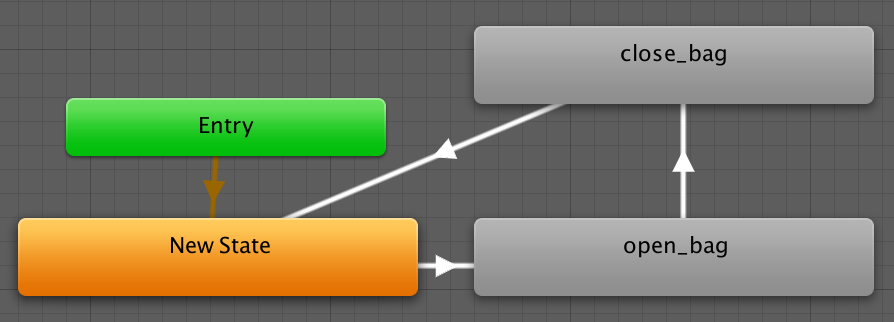
\includegraphics[width=0.35\textwidth]{images/animator.png}
        \captionof{figure}{Screenshot of the animator component attached to each animated object in the CG-environment.}
        \label{animator}
    \end{center}
\end{minipage}

\subsection{Deployment}
Unity offers the ideal environment to build directly to Android. This is done by installing the Android SDK, setting the XR Settings in Player Settings to Google Daydream, then building to the Android Platform. 


\section{Memory Test}
\subsection{Site Overview}
In order to allow users to complete the memory test, and submit their results remotely, a static website was constructed. Using a static site meant that the site could be hosted by GitHub pages \footnote{GitHub Pages | Websites for you and your projects \url{https://pages.github.com/}}. The only requirement of the site is that a user can complete the memory test and submit their results. To ensure that any submitted results are verified that they have come from a specific user, a user must first have to sign in. Once a user has signed in. Once a user has signed in, their results must be submitted to and stored in a database, along with their user id. To enable the use of the following APIs within a static website the JavaScript tool Browserify was used. This tool bundles all dependencies into a single \lstinline{bundle.js} file.  

\subsection{Web Technologies}

\subsubsection{Google OAuth}

Using Google OAuth, a site can have authentication and sign in functionality. Google's API uses the OAuth 2.0 protocol to authenticate and authorise. To enable the use of Google OAuth, the following meta and script tags must be inluded in the head of the HTML file. 

\noindent \begin{minipage}{\textwidth}
\centering
\begin{lstlisting}
<meta name="google-signin-scope" content="profile email"/>
<meta name="google-signin-client_id" content="[YOUR _CLIENT_ID_HERE].apps.googleusercontent.com"/>
<script src="https://apis.google.com/js/platform.js" async defer></script>
\end{lstlisting}
\end{minipage}

Using this API, a button is placed within the site with the class \lstinline{g-signin2} which a user uses to sign in - as seen in Figure \ref{web-design}. After a user is signed in, the API returns that user's email address. This email address is then sent with the user's results on submission. Google's API returns a \lstinline{googleUser} object, from which the user's email can be retrieved and stored. 

\bigskip
\noindent \begin{minipage}{\textwidth}
\centering
\begin{lstlisting}
window.onSignIn = function(googleUser) {
  var profile = googleUser.getBasicProfile();
  var email   = profile.getEmail();
}
\end{lstlisting}
\end{minipage}


\subsubsection{Firebase Database}
Due to the static nature of the site, there is no server-side code, thus it is non-trivial to construct a secure database to store the submissions from the user study. The solution chosen for this application is Firebase Realtime Database \footnote{Firebase Realtime Database \url{https://firebase.google.com/docs/database/}}. This is a NoSQL cloud database. All data within this database is stored as JSON. In order to to enable the use of Firebase, the following script tag must be used within the HTML file:

\noindent \begin{minipage}{\textwidth}
\centering
\begin{lstlisting}
<script src="https://www.gstatic.com/firebasejs/4.10.1/firebase.js"></script>
\end{lstlisting}
\end{minipage}

Once a user has completed their test, they click the submit button which calls \lstinline{saveMessage} as shown below.

\bigskip
\noindent \begin{minipage}{\textwidth}
\centering
\begin{lstlisting}
function saveMessage(email, right, wrong) {
  var newResponseRef = ref.push();
  newResponseRef.set({
    email:email,
    right:right,
    wrong:wrong
  });
};
\end{lstlisting}
\end{minipage}

\subsection{CSS}
Since the site was designed to have a single user flow, the only design decision that was to be made was how the question were to be presented to the user. Following the general structure of the memory test outlined by CANTAB's library of cognitive tests - which is discussed further in Subsection \ref{cantab} - each question must be presented one by one; the user can only proceed if they answer correctly. This is done by simply having hidden HTML elements, which are set to visible in the order that they exist in the HTML file. Using the class name \lstinline{question} for every question means that the element selector \lstinline{document.getElementsByClassName('question');} will return an array of all questions. Now, on a correct answer, we can set the current question to the css display \lstinline{hidden} and set the next question to \lstinline{block}.

\begin{minipage}{\textwidth}
\centering
\begin{lstlisting}
window.Right = function() {
  sections = document.getElementsByClassName('question');
  sections[question].style.display = 'none';
  question++;
  sections[question].style.display = 'block';
};
\end{lstlisting}
\end{minipage}

The second requirement of this site is that it should be usable on mobile. Modern CSS functionality makes this task trivial for a static site. Using only the \lstinline{rem} unit of measurement ensures that all elements are scaled and positioned relative to the size of the viewing device. It is important to ensure the use of the meta tag \lstinline{<meta name="viewport" content="width=device-width, initial-scale=1"/>} to correctly scale to smaller devices. 


\ subsection{Web Design}


\begin{center}
    \centering
    \begin{minipage}{0.3\textwidth}
        \centering
        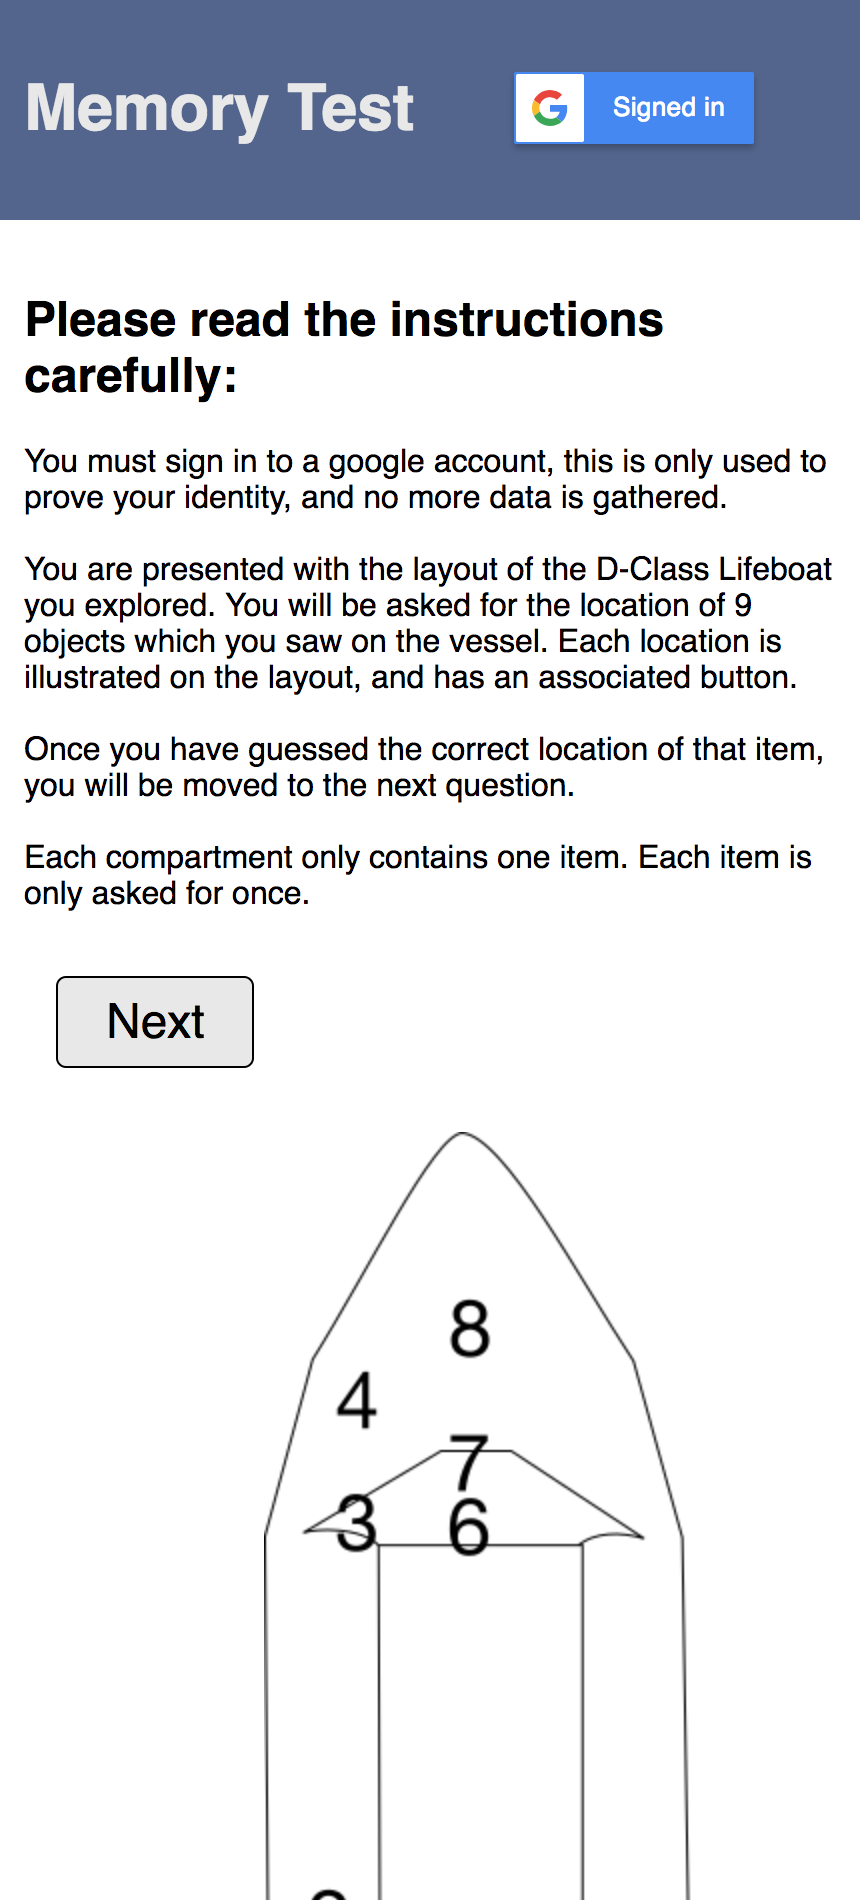
\includegraphics[width=1\textwidth]{images/web-intro.png}
    \end{minipage}\hfill
    \begin{minipage}{0.3\textwidth}
        \centering
        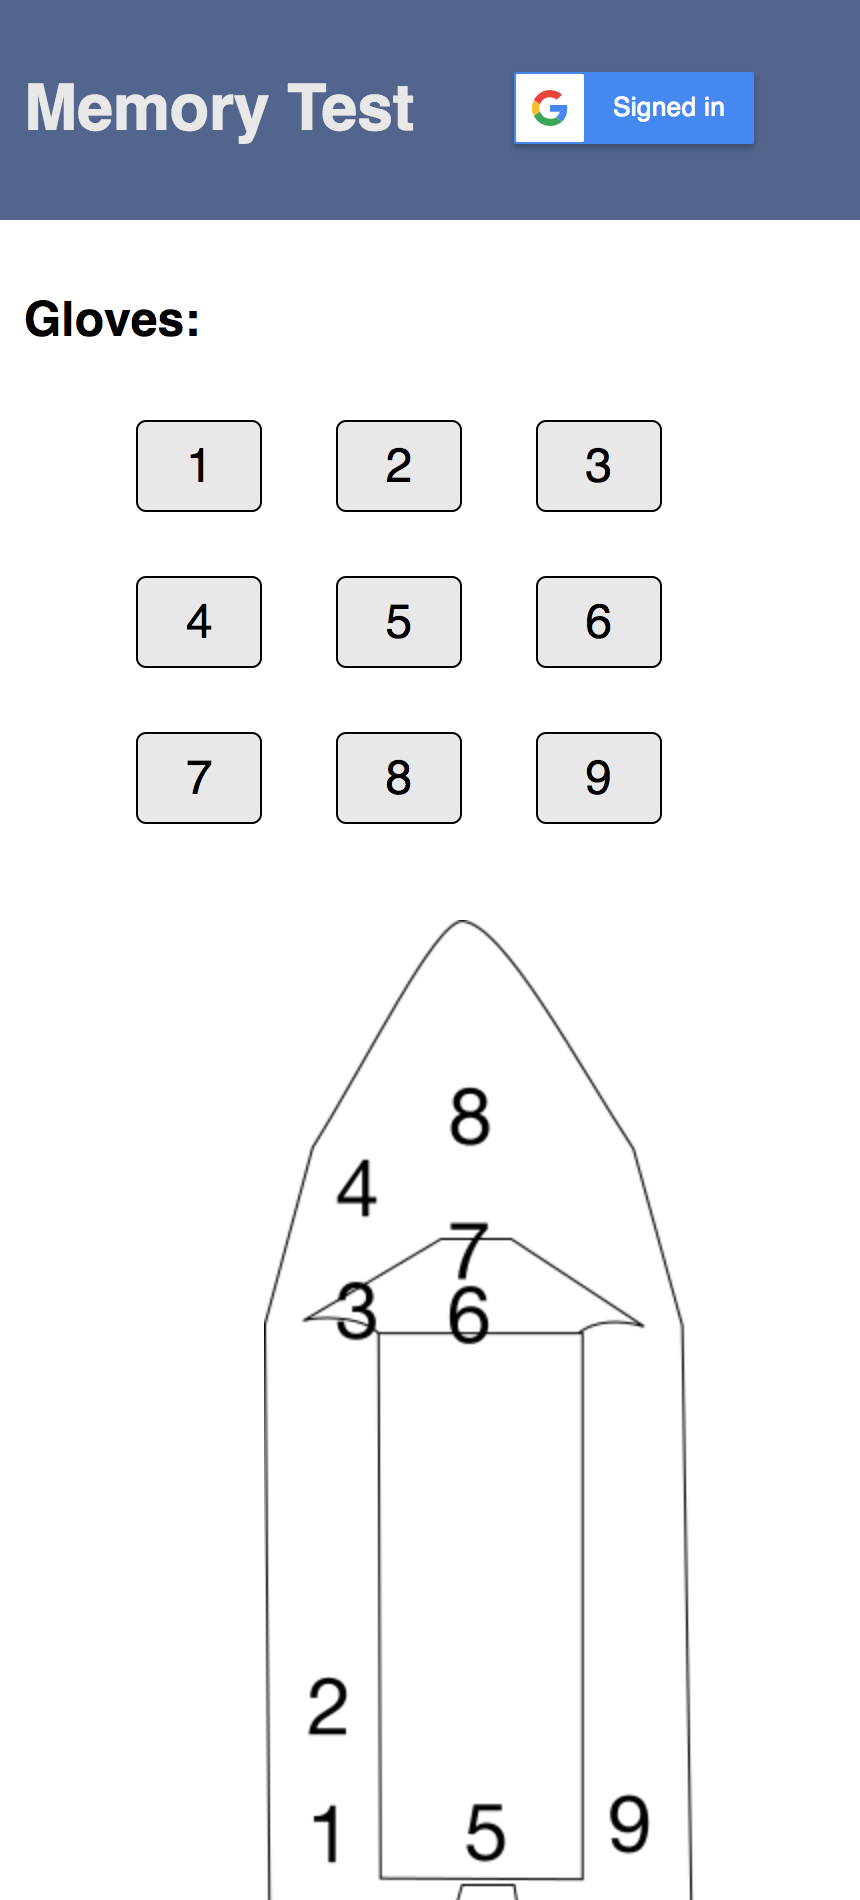
\includegraphics[width=1\textwidth]{images/web-question.png}
    \end{minipage}\hfill
    \begin{minipage}{0.3\textwidth}
        \centering
        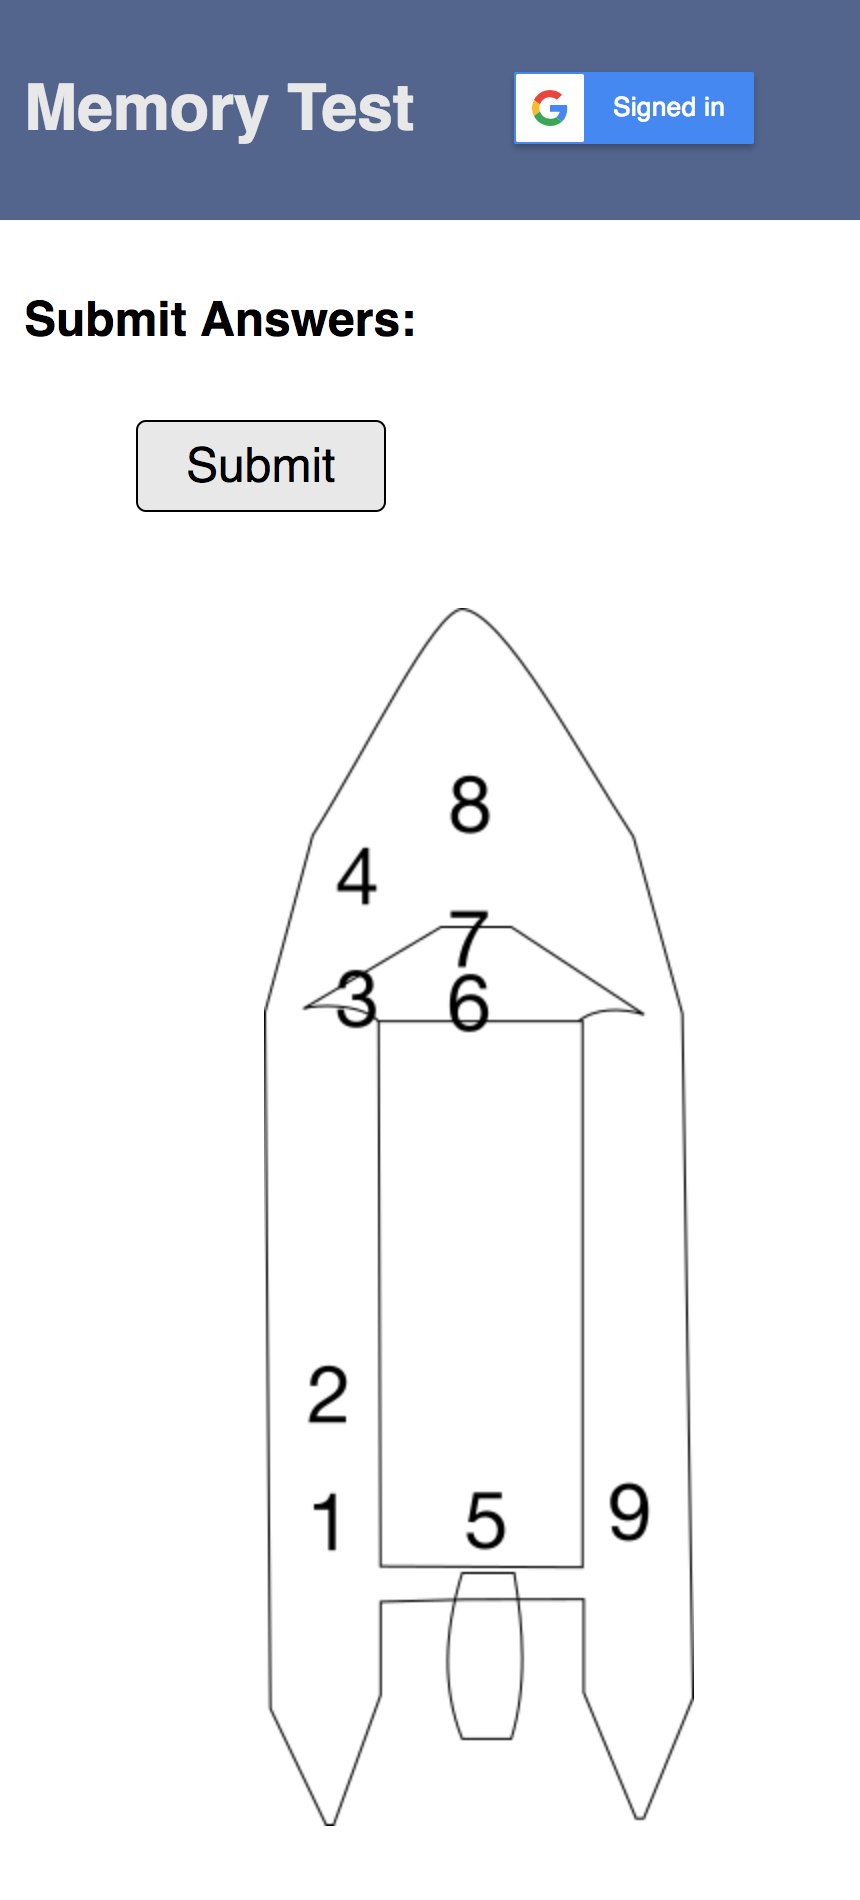
\includegraphics[width=1\textwidth]{images/web-thanks.png}
    \end{minipage}\hfill
    \captionof{figure}{Screenshots of the three stages a user follows in order to complete the memory test.}
    \label{web-design}
\end{center}
























\chapter{User Study, Analysis, and Evaluation}\label{user-study-chapter}

\section{User Study Design}

\subsection{Considerations}
In order to conclude the effectiveness of each of the training experiences in the transfer of spatial awareness a user study must be conducted. One of the few considerations for the design of the study is the effect of learning, which in this case is the focus of the study.

There are many variables associated with the effectiveness of the transfer of spatial awareness, as discussed in Section \ref{intro-summary}. In a perfect study, these factors would be individually isolated. Unfortunately, in this instance it was not possible, and many of these factors remain a consideration when determining the cause of any disparity in training performance. Although, responsiveness, and interactivity were both possible to isolate from the study. Thus, Accuracy, Fidelity, and Presence remain the only independent variables, which are altered between each medium. 

The 360-image training environment has an increased accuracy, and fidelity. Hypothetically, due to the lack of stereoscopic vision users will experience a reduced sense of presence. This does in fact prove to be the case, and the comparison between stereoscopic vision and monoscopic vision is discussed further in a later section, Section \ref{stereo}
The computer-generated training environment has a lower accuracy, and fidelity, but hypothetically, a heightened sense of presence. 

Although, a significant difference between the two environments is the overall complexity of the scene. In the 360 environment, a users is surrounded by an environment with a much higher complexity with many objects in the scene which are not required for recall. The CG environment places the user in a far less complex scene where there a little or no objects in the scene which are not required for recall.

\subsection{Hypothesis}\label{hypothesis}
I hypothesise that the inherently reduced complexity, coupled with the stereoscopic vision will yield improved transfer of spatial awareness for users which experience the CG scene.

\subsubsection{Null Hypothesis}
With this in mind it is possible to construct the null hypothesis that there will be no difference in the error count of users which have been trained in the CG environment and in the 360 environment.


\subsection{Method}\label{cantab}
The subjects chosen for this study were chosen at random from individuals at the University of Bristol, with no prerequisites, in a Hallway testing manner. This lead to a consistent mix of individuals mostly in the demographic of students from age of 18-25. 20 subjects were tested, with 18 completing the week later memory test. Although there was little or no choice for test subjects, this group is a fair representation of the target audience of this training application, and importantly most students in this age range will have similar experience in video gaming, and thus should not effect the results in this small sample size. Although, there is a discussion to be had with regards to potential disparities between males and females participating in spatial memory studies. 

In order to negate the effect of learning for participants, an in-between groups user study is the only option, although this unfortunately doubles the required sample size, and reduces the statistical power of  each user's results. 

In order to assess the spatial memory of a user, CANTAB's Library of cognitive tests was referenced in order to determine an appropriate strategy. "Spatial Working Memory requires retention and manipulation of visuospatial information. This self-ordered test has notable executive function demands and provides a measure of strategy as well as working memory errors" \footnote{ CANTAB: Spatial Working Memory (SWM) Test \url{https://goo.gl/W7NTSM}}. Thus a similar, simple test was constructed in the training environments. 

\subsection{Task}
Users are placed in one of the two training environments. In each of these two environments, there are 9 labelled objects located in the scene. The user is able to interact with each object to the extent that they are able to click on the object, and their location changes to near the object. The user is given 2 minutes in order to memorize these objects. After 2 minutes, the user exits the environment, they then immediately complete a memory test for the location of each of the 9 objects in the scene. Their performance, namely error rate, is recorded. A week later, the study participant will once again complete an identical memory test, and again their performance is recorded. In the memory test, the user is presented with the layout the D-Class Lifeboat, with 9 potential locations. The user is informed that each of these locations contains exactly one item. Figure \ref{layout-diagram} shows the diagram the participants are shown. 

\begin{minipage}{\textwidth}
\hfill \break
\centering

\includegraphics[width=0.2\textwidth]{images/ilb_simple}
\captionof{figure}{Diagram of the D-Class Lifeboat, with 9 locations illustrated}
\label{layout-diagram}
\hfill \break
\end{minipage}
\newpage
\section{Results}
Below are the results of the user study. 

\begin{minipage}{\textwidth}
    \centering
    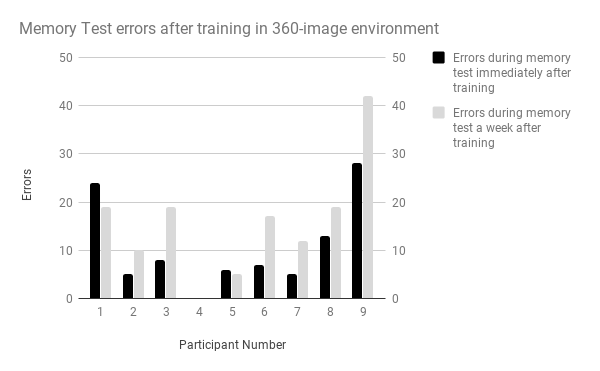
\includegraphics[width=0.8\textwidth]{images/results-360} % first figure itself
    \captionof{figure}{Memory test error count for each participant that trained in the 360-image environment, each bar representing the error count for the immediate memory test, and week later memory test}
    \label{res-360}
\end{minipage}

\begin{minipage}{\textwidth}
    \centering
    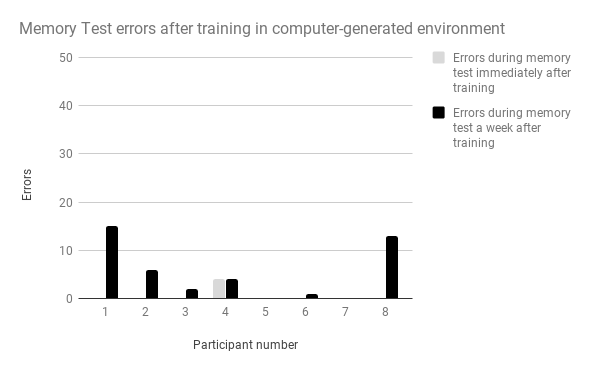
\includegraphics[width=0.8\textwidth]{images/results-CG} % second figure itself
    \captionof{figure}{Memory test error count for each participant that trained in the computer-generated environment, each bar representing the error count for the immediate memory test, and week later memory test}
    \label{res-CG}
\end{minipage}

\begin{minipage}{\textwidth}
    \centering
    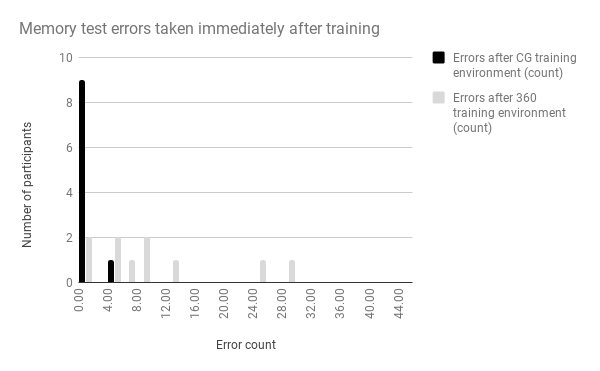
\includegraphics[width=0.8\textwidth]{images/immediate-histo} % first figure itself
    \captionof{figure}{Histogram of the error count of participants during the memory test taken immediately after training, for participants from each group}
    \label{imm-res}
\end{minipage}


\begin{minipage}{\textwidth}
    \centering
    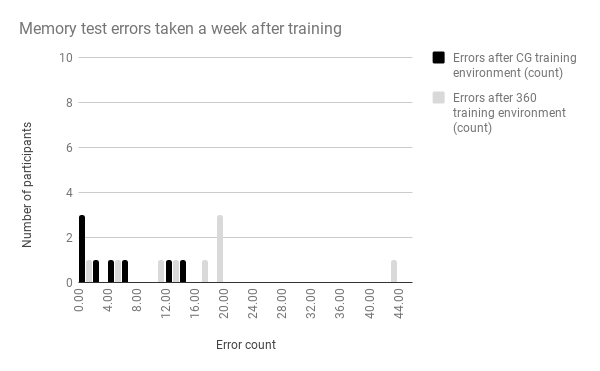
\includegraphics[width=0.8\textwidth]{images/week-after-histo} % second figure itself
    \captionof{figure}{Histogram of the error count of participants during the memory test taken a week after training, for participants from each group}
    \label{week-res}
\end{minipage}


\begin{table}[ht!]
\centering
\caption{Each value represents the amount of errors each user made when recalling the location of 9 items.}
\label{my-label}
\begin{tabular}{l
>{\columncolor[HTML]{FFFFFF}}c 
>{\columncolor[HTML]{FFFFFF}}c 
>{\columncolor[HTML]{FFFFFF}}c 
>{\columncolor[HTML]{FFFFFF}}c }
                             & \multicolumn{2}{c}{\cellcolor[HTML]{FFFFFF}{\color[HTML]{333333} CGI}}                                                             & \multicolumn{2}{c}{\cellcolor[HTML]{FFFFFF}{\color[HTML]{333333} 360}}                                                             \\ \cline{2-5} 
\multicolumn{1}{l|}{}        & \multicolumn{1}{l|}{\cellcolor[HTML]{FFFFFF}Initial Recall Task} & \multicolumn{1}{l|}{\cellcolor[HTML]{FFFFFF}Recall Task after 1 Week} & \multicolumn{1}{l|}{\cellcolor[HTML]{FFFFFF}Initial Recall Task} & \multicolumn{1}{l|}{\cellcolor[HTML]{FFFFFF}{Recall Task after 1 Week}} \\ \hline
\multicolumn{1}{|l|}{Mean}   & \multicolumn{1}{c|}{\cellcolor[HTML]{FFFFFF}0.5}            & \multicolumn{1}{c|}{\cellcolor[HTML]{FFFFFF}5.125}                   & \multicolumn{1}{c|}{\cellcolor[HTML]{FFFFFF}10.667}         & \multicolumn{1}{c|}{\cellcolor[HTML]{FFFFFF}15.889}                  \\ \hline
% \multicolumn{1}{|l|}{Median} & \multicolumn{1}{c|}{\cellcolor[HTML]{FFFFFF}0}              & \multicolumn{1}{c|}{\cellcolor[HTML]{FFFFFF}3}                       & \multicolumn{1}{c|}{\cellcolor[HTML]{FFFFFF}7}              & \multicolumn{1}{c|}{\cellcolor[HTML]{FFFFFF}17}                      \\ \hline
\end{tabular}
\end{table}

\subsection{Analysis}
For the initial recall task and recall task 1 week after, a two-tailed t-test revealed a significant difference between the number of errors made by users trained in the CG environment (M = 0.5, SD = 1.41) (M = 5.13, SD = 5.87),  and users trained in the 360-image environment (M = 10.67, SD = 8.49)(M = 15.89, SD = 12.66); t(18) = 0.013 for initial recall, and t(16) = 0.01 for recall one week after. Therefore it is possible to reject the null hypothesis, in favour of the hypothesis described in Section \ref{hypothesis}

\section{Evaluation}
These results prove that the computer-generated environment was far superior to the 360-image environment in the training of participants for this specific task. Not only did participants that were trained in the CG environment perform considerably better during the memory test taken immediately after, this group were able to recall the layout of the vessel better after a week than the participants which were trained in the 360-image environment could immediately after training. Suggesting that this group were able to acquire a deeper spatial awareness than that of the second group. 

Although this has proven conclusively that the computer generated training environment was superior, it is difficult to conclude the cause of this superiority. The main functional factors which likely lead to this difference are, Scene Complexity and noise, and Stereoscopic vision. Other factors which may have influenced these results are discussed in Section \ref{discussion}.

\subsection{Scene Complexity}

The disparity between the two environments for scene complexity is quite substantial. In the CG environment, the user is presented with only simple textures, and a monotonic background scene. The 3D model is only populated with crucial items, in addition to the items to be recalled. Whereas in the 360-image environment, the background scene is complex, and the boat is littered with many - potentially distracting - elements. Although this may be have been a factor in the acquisition of spatial awareness, it is difficult to determine quantitavely how much this influenced the results. In this instance - where a user must recall the scene purely from memory, with no prompts - it is fair to conclude that increased complexity of the scene was likely detrimental to performance in memory tests. But, crucially, there is a discussion to be had on the effect of context on spatial cognition. In particular, users which experienced the 360-image environment may have performed better if they were recalling the items whilst actually on the vessel, as they had been trained with a more realistic environment. Further discussion on this is had in Section \ref{context}.

\subsection{Stereoscopic Vision}\label{stereo}
Potentially the most substantial difference found between the two presentation media is the difference between monoscopic and stereoscopic vision. There is little literature on the comparison of stereoscopic and monoscopic vision and its effect on spatial cognition, and literature that does exist has given mixed results \citep{price}. Although, no studies were discovered which had compared these media using a VR headset for both environments. 

From anecdotal user feedback there existed a disparity between a user's immersion within each of the environments, and thus their sense of presence within said environment. Users reported feeling that they were "just looking at a picture" when experiencing the 360 environment. Whereas, in the CG environment users often found it more immersive, and disorienting once they exited the scene; suggesting they had become more present within the virtual environment. It is not be possible to determine conclusively to what extent this effects a user's retained and working spatial memory, but it is reasonable to suggest that it is significant. This could be easily concluded with further study, this is discussed further in Section \ref{further}. 


\chapter{Discussion, Conclusion, and Future Work}


\section{Discussion}\label{discussion}

\subsection{Context}\label{context}
The environment in which user's recall their training is crucial. In a study by \cite{Godden1975} which trained participants above and below water, participants who were taught underwater better recalled that training when underwater, and vice versa. Thus, it would be fair to assume that although the CG led to less user errors in a neutral environment for recall, it is likely that the errors made by users from the 360-image environment would be reduced if they were to be recalled whilst actually on the vessel; since they had been trained in a seemingly identical environment. With this in mind, it would be difficult to say which environment would translate to better results in the real world, as discussed in Section \ref{further}, further study would be required to conclude this. 

\subsection{Novelty}\label{novelty}
"When experiencing a novel environment ... people are typically more aroused and broadly focused on the tasks to be performed or the situation to be experienced" \citep{Witmer1998}. Anecdotally, participants which used the CG environment were generally far more enthused by the experience. Although the 360 environment is an interesting experience it did not seem to be as engaging for users. This could be theorised to be caused by the lack of stereoscopic vision making the experience less immersive, or that the simpler scene made it more easy to engage with. Although, I would speculate that this is most likely caused by the fact that the CG environment is a more novel experience, in comparison to the 360-scene which may seem like a picture gallery. 

This factor of novelty makes the results biased in favour of the CG environment. An implemented training application using the CG environment would not maintain this novelty as users become more accustomed to the use of it. The added expense of constructing a CG environment in contrast the 360 environment may not be worth it once this novelty dissipates, and should be considered for further study. 

\subsection{Application}

In order to determine the success of the application it is useful to refer back to the requirements of the application stated in Section \ref{requirements}, which were as follows:

\begin{itemize}
    \item Affordable
    \item Accessible
    \item Effective
\end{itemize}

\subsubsection{Affordable}
The most successful aspect of this project was proving the affordability of creating a virtual training application. With respect to hardware, the costs associated with implementing a virtual training environment have plummeted. At the beginning of this project, the most viable solution to interacting with a VR environment was the Google Daydream View HMD, which was the HMD of choice throughout this project. In the last 8 months, since the beginning of this project, HMDs have taken another step. This step comes in the form of the first standalone VR HMD - the Oculus Go \footnote{Oculus: Go \url{https://www.oculus.com/go/}}; this means the headset works completely wirelessly, and without the requirement of a smartphone device. The lack of a smartphone device halves the total cost of the setup. 

From a software development standpoint, a fully functional deployment would clearly be associated with costs far greater than that of the hardware associated with using it. Without an in-house development team it is likely that these costs would be difficult for the RNLI to justify without further study. But, as proven throughout this project, modern development platforms enable the construction of complex applications in shorter times than previously possible. Over time, the costs associated with developing virtual training applications will fall in a similar fashion to the costs of hardware.

\subsubsection{Accessible}
Due to the mobile nature of modern HMDs, a well deployed version of these applications would be easily accessible to Lifeboat stations nationally. Each station would need a modern smartphone device, and a Google Daydream View HMD. With only this equipment, a station and its crew would be able to access a fully functional virtual training environment. This is in stark contrast to the static virtual training environment which is based in RNLI Headquarters in Poole. 

\subsubsection{Effective}
The user study conducted proved that users a capable of learning and retaining knowledge of the layout of the D-Class after just 2 minutes experience of the CG environment. Further studies are required to conclude how well this translates to the real world, but preliminary results have proven promising. 

\subsection{User Study}
The user study proved, with a strongly significant result, that the CG environment helped users recall - and retain knowledge of - the layout of the boat considerably better than the 360 environment was capable of doing. As discussed, the key controlled factors which may have caused this disparity are the difference of stereoscopic and monoscopic display, and simple and complex scenes. The effect of these factors could be quantified with further study, which is discussed in Section \ref{further}. Another factor which may or may not have effected performance is that of context of recall, as discussed in Section \ref{context}; this could similarly be accounted for as discussed in Section \ref{further-context}. Finally, novelty may have affected the effectiveness of each application (Section \ref{context}), since users may have been more engaged with the more novel CG environment. The effect of novelty could be approached in a qualitative study. 

\section{Conclusion}
To conclude, it is pertinent to refer back to the primary research questions as stated in Section \ref{tech-summary}:

\begin{itemize}
    \item Which technological approach, if any, is the most effective way for the RNLI to train crew members in a virtual environment?
\end{itemize}

The user study concluded that in this task, the most effective way to train individuals was with a computer-generated environment. The RNLI, or similar organisations, should conduct further investigation into the effectiveness of computer-generated virtual reality environments. 

\section{Future Work}\label{further}
\subsection{Computer-Generated Environment}
The CG environment application developed during this project has a broad scope for further development. Much of that scope is a necessary step that must be taken to construct a complete application, such as menu's and UI elements, further 3D models, and further training units. 

For further 3D models, each of the vessels available in the fleet would need to be reconstructed in 3D. Conveniently, the RNLI fleet is currently in the process of modernisation. The future fleet of vessels which will require a volunteer crew will consist of the D-Class, B-Class, Shannon, and Tamar class lifeboats. Each of these vessels are considerably more complex than the D-Class model constructed in this project, but a 3D model would only need to be constructed once, and would serve more purposes than to simply be used in the training application. 

The entire list of assessment units in the crew training programme are possible to implement in the virtual training environment. With that said, there are specific units which would be most benefited by the use of a virtual training implementation. These units are the units which typically are associated with excessive cost or danger. In particular, capsize drills would be an appropriate unit to replicate in a virtual training environment. 

\subsection{360-Degree Image Environment}
The considerable improvement that could be made to the 360-image environment is the use of more sophisticated technology to capture the 360-degree. Specifically, the use of a 3D 360-degree camera would enable the development of a stereoscopic 360-image environment. This would allow for the construction of a considerably more immersive environment, which would potentially give users a greater sense of presence within the scene. 

\subsection{Context}\label{further-context}
With respect to future academic work, there are many unanswered questions. Most fundamentally is the effect of context in the recall of items. 3D environments have been proven to be superior when recall will be required in a neutral environment, with minimal visual guides. But, it is not yet conclusive how these results would transfer to the real world, where the 360-image training environment would be considerably more similar to the environment in which the users would be expected to recall the spatial properties of the environment. A study where users are asked to recall the spatial properties of the environment while they are on the vessel, should be able to determine shed light on the impact if this factor on the training of spatial ability. 

\subsection{Route, and Survey Knowledge}
Further study into the training capabilities of potential virtual environment has a large scope. This project was focussed on the training and testing of a user's landmark knowledge of an environment, and their ability to recall those landmarks, it did not observe into the training of a person's route or survey knowledge. In order to do this, a further study could be undertaken which assesses a user's patch knowledge; knowledge of the patch of coastline that the trainees Lifeboat station is responsible for.

Testing patch knowledge requires the user to travel around a small geographical area, this would typically be a harbour or coastline. This area consists of multiple landmarks and hazards, such as piers, beaches, boats, and rocks. The user must remember these landmarks, and be able to travel between them, utilising their landmark, route, and survey knowledge acquired of the area. 


% \begin{appendices}
% \chapter{Interviews}
% \section{Participant A}
% \section{Participant B}
% \end{appendices}

\clearpage
\bibliography{Dissertation.bib}

% \end{multicols}
\end{document}